%% =====================================================================
%% main-llmxive.tex — content-extracted llmXive wrapper
%% =====================================================================
%% Generated by scripts/extract_paper_content.py. The original paper
%% body is preserved; the venue-specific preamble (class, bundled .cls
%% files, custom packages) is DISCARDED and replaced with the llmxive
%% house style + a shim block that no-ops any venue-specific macros the
%% body still references.
%% =====================================================================
\documentclass{llmxive}


%% ── Packages forwarded from original preamble ─────────────────
\usepackage{graphicx}
\usepackage{subcaption}
\usepackage{makecell}
\usepackage{multirow}
\usepackage{colortbl}
\usepackage{wrapfig}
\usepackage{enumitem}
\usepackage{tcolorbox}
\usepackage{url}
\usepackage{amsmath}
\usepackage{amssymb}
\usepackage{amsfonts}
\usepackage{mathtools}
\usepackage{amsthm}
\usepackage[capitalize,noabbrev]{cleveref}
\usepackage{float}
\usepackage{placeins}
\usepackage{natbib}

%% ── Shim layer (venue macros made into no-ops) ────────────────
\makeatletter
\providecommand{\TODO}[1]{}
\providecommand{\abscontent}{}
\providecommand{\absfont}{}
\providecommand{\acknowledgments}{\section*{Acknowledgments}}
\providecommand{\address}[1]{}
\providecommand{\affiliation}[1]{}
\providecommand{\aistatsfinalcopy}{}
\providecommand{\animategraphics}[5][]{\includegraphics[#1]{#3#4}}
\providecommand{\argmax}{\mathop{\mathrm{arg\,max}}}
\providecommand{\argmin}{\mathop{\mathrm{arg\,min}}}
\providecommand{\authornote}[1]{}
\providecommand{\authornotemark}[1][]{}
\providecommand{\authorrunning}[1]{}
\providecommand{\blfootnote}[1]{\footnote{#1}}
\providecommand{\bm}[1]{\boldsymbol{#1}}
\providecommand{\corresponding}{}
\providecommand{\correspondingauthor}[1]{}
\providecommand{\eg}{e.g.,\xspace}
\providecommand{\email}[1]{\href{mailto:#1}{#1}}
\providecommand{\equalcontribution}{}
\providecommand{\etal}{et al.\xspace}
\providecommand{\etc}{etc.\xspace}
\providecommand{\iclrfinalcopy}{}
\providecommand{\icmlfinalcopy}{}
\providecommand{\ie}{i.e.,\xspace}
\providecommand{\iid}{i.i.d.\xspace}
\providecommand{\institute}[1]{}
\providecommand{\keywords}[1]{\par\noindent\textbf{Keywords:} #1}
\providecommand{\neuripsfinalcopy}{}
\providecommand{\orcid}[1]{}
\providecommand{\tablecite}[1]{\cite{#1}}
\providecommand{\theabstract}{}
\providecommand{\titlerunning}[1]{}
\providecommand{\todo}[1]{}
\providecommand{\wrt}{w.r.t.\xspace}
\AtBeginDocument{\renewcommand{\and}{ \textperiodcentered\ }}
\makeatother

%% ── User-defined macros forwarded from original preamble ─────
\makeatletter
\providecommand{\theHalgorithm}{\arabic{algorithm}}
\providecommand{\@notice}{\enlargethispage{2\baselineskip}}
\providecommand{\ciSE}[2]{}
\providecommand{\ciSEB}[2]{}
\providecommand{\ciAdvInf}[2]{}
\providecommand{\ciAdvNS}[2]{}
\providecommand{\ciAdvInfB}[2]{}
\providecommand{\ciAdvNSB}[2]{}
\providecommand{\arraystretch}{1.2}
\definecolor{okabeOrange}{HTML}{D55E00}
\definecolor{okabeBlue}{HTML}{0072B2}
\definecolor{c4low}{HTML}{F4D8C8}
\definecolor{c4high}{HTML}{D6E8F4}
\newtcolorbox{runex}{
  colback=gray!5,
  colframe=gray!40,
  arc=2pt, boxrule=0.4pt,
  left=6pt, right=6pt,
  top=4pt, bottom=4pt,
  title=Running Example,
  fonttitle=\bfseries\small,
  coltitle=black,
  colbacktitle=gray!15,
}
\makeatother

%% ── llmXive paper metadata ──────────────────────────────────
\title{Formalizing Latent Thoughts: Four Axioms of Thought Representation in LLMs}
\author{Fahd Seddik \and Fatemeh Fard}
\paperid{arXiv:2606.27378}
\paperstatus{Preprint}

\begin{document}
\maketitle
\begin{abstract}
We introduce an axiomatic evaluation framework for latent thought representations in LLMs, comprising metrics that are independent of downstream benchmark scores and reveal representational failures that benchmark accuracy masks. Existing evaluations conflate representation quality with model capacity. Therefore, failures cannot be attributed to the representation rather than to the model that processes it. We formalize four functional axioms (Causality, Minimality, Separability, and Stability) and define a quantitative measure for each, computed directly on the representation independently of downstream accuracy. We audit open-weight LLMs across 23 reasoning tasks (e.g., Spatial Reasoning, Factual QA). We find that no candidate satisfies all four axioms simultaneously, that the representations distinguish task type reliably but cannot distinguish between two questions within the same task, and that the representations encode little information beyond what is already present in the input embedding. The failure is consistent across dense, reasoning-distilled, and RL-trained model families, indicating that the gap is structural rather than a property of model size or training procedure. Code: \url{https://fard-lab.github.io/formalize-thoughts}.
\end{abstract}
\etocdepthtag.toc{main}





\section{Introduction}
\label{introduction}

Reasoning in Large Language Models (LLMs) has increasingly moved from discrete Chain-of-Thought (CoT) tokens toward continuous latent representations, with a growing body of efficiency-motivated work compressing or replacing explicit CoT steps with continuous vectors~\citep{sui2025stopoverthinkingsurveyefficient, feng2025efficientreasoningmodelssurvey}. Recent work highlights the limitations of discrete tokenization and decoding for reasoning~\citep{hao2024training} and replaces discrete steps with continuous representations~\citep{butt2026soft, zhang2025softthinkingunlockingreasoning}, reporting accuracy gains on complex reasoning benchmarks~\citep{wu2026llms}. However, the field evaluates these ``continuous thought representations'' almost exclusively through downstream task accuracy~\citep{mondorf2024accuracyevaluatingreasoningbehavior}. Probes of continuous reasoning tokens find that distinct reasoning paths collapse to a single interpretation in early layers while downstream accuracy remains unchanged~\citep{rizvi-martel2026the}. Two prior questions therefore remain open. What functional properties constitute a valid thought representation, and how can we measure those properties independently of any downstream task? Even when models maintain accurate internal representations, they may fail at downstream tasks~\citep{ye2026mechanistic}.

\begin{figure}[t]
    \centering
    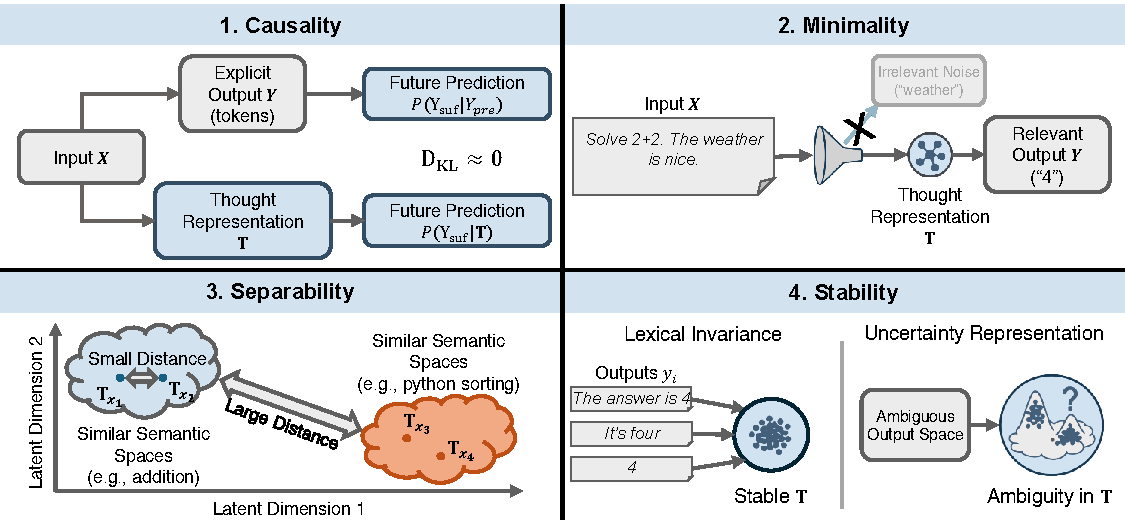
\includegraphics[width=\linewidth]{figures/pdf/characteristics.pdf}
    \vspace{-10pt}
    \caption{Visualizing the axiomatic properties of a Functional Thought Representation $\mathbf{T}$}
    \label{fig:characteristics}
    \vspace{-10pt}
\end{figure}


We identify three gaps that impede principled progress on continuous reasoning. First, there is no \textbf{principled definition} of what a thought representation must do, because existing methods optimize heuristic proxies (step counts, token budgets, imitation of explicit CoT) without a formal statement of the functional requirements. Second, there is no \textbf{intrinsic evaluation} that measures representation quality independently of downstream accuracy~\citep{sahoo2026when}, and therefore failures cannot be attributed to the representation rather than to the decoder or prompt. Third, and consequently, the \textbf{status of current methods} is unknown. Recent audits find that latent reasoning tokens are often unnecessary for the predictions they are meant to drive~\citep{dilgren2026are}, and that latent reasoning does not faithfully implement the structured latent-space search that motivates it~\citep{cui2026how}.

\textbf{Our approach.} We propose an axiomatic characterization of thought representations in terms of four functional properties (\emph{Causality}, \emph{Minimality}, \emph{Separability}, and \emph{Stability}), illustrated in Figure~\ref{fig:characteristics}. The framework describes the function of a thought representation rather than its form. It applies equally to vectors, tensors, or sets of vectors. For each axiom, we define a quantitative measure evaluated directly on the source LLM without retraining. We use this suite to audit candidate thought representations produced by Soft Thinking with and without Gumbel noise~\citep{zhang2025softthinkingunlockingreasoning, wu2026llms} and Latent Thinking~\citep{hao2024training, zou2025latentcollaborationmultiagentsystems} across a range of thinking budgets, alongside candidates extracted from last-input-token hidden states. We study five open-weight LLMs spanning dense and sparse mixture-of-experts architectures on the 23 tasks of Big Bench Extra Hard (BBEH)~\citep{kazemi2025bigbenchextrahard}.

Across the evaluated source LLMs, the intrinsic protocol exposes failure modes that downstream task accuracy does not. The candidates retain coarse task identity but lose the per-question identity that distinguishes one instance of a task from another, and the input-prompt embedding is itself competitive with the candidates on every axis the framework measures.

\textbf{Contributions.} Each of the three gaps above is addressed by a corresponding contribution.
\begin{itemize}
    \item \textbf{Axiomatic formalization of thought representations.} We provide a definition of thought representations stated in terms of four functional axioms, and prove their logical consistency, independence, and completeness (Appendix~\ref{appendix:theoretical_properties}).
    \item \textbf{Intrinsic evaluation protocol.} We introduce a measure for each axiom. KL substitution error measures Causality, the Minimality Gap measures Minimality, same- and cross-task discriminator accuracy measures Separability, and the Distributional Consistency Score (DCS) measures Stability. Each measure is computable on the source LLM without retraining and is decoupled from downstream task accuracy.
    \item \textbf{Empirical audit of candidate thought representations.} Applying the protocol on BBEH exposes a fine-grained \emph{representational collapse} on per-question identity. No evaluated candidate satisfies all four axioms simultaneously, consistent with concurrent reports of silent representational failures in latent reasoning despite unchanged downstream accuracy~\citep{sahoo2026when}.
\end{itemize}

The framework provides a principled means to develop and audit candidate thought representations as objects of study, evaluated for what an LLM encodes about a problem rather than for the downstream reasoning quality of any chain that follows. Beyond evaluation, the four measures provide researchers explicit, quantifiable optimization targets and the diagnostic resolution to attribute downstream accuracy changes to specific representational properties rather than to an aggregate benchmark score. The four measures are one realization of the axioms, which admit alternative quantifications under the same principle, allowing new candidates and measurement designs in future work.

\section{Related work}
\label{related work}

\textbf{Latent representations.} Probing studies demonstrate that LLMs build rich internal representations before outputting tokens, with internal states predicting CoT success prior to completion~\citep{afzal2025knowingsayingllmrepresentations, lugoloobi2026llms}, encoding sparse logical features~\citep{helff2026activationreasoning}, and correlating with task difficulty~\citep{herrmann2025measuring}. These internal signals motivate representations capturing model intent without reliance on explicit outputs. COCONUT~\citep{hao2024training} and CODI~\citep{shen2025codicompressingchainofthoughtcontinuous} utilize hidden states to represent or compress multiple reasoning paths into continuous vectors. Architectural variants including Tiny Recursive Models (TRMs)~\citep{jolicoeurmartineau2025morerecursivereasoningtiny, wang2026tiny} and Encode-Think-Decode (ETD)~\citep{koishekenov2025encodethinkdecodescaling} update latent representations via recursive networks or iteration over reasoning-relevant layers, and related models propagate persistent latent state~\citep{li2026learning} or inject recurrence through a dedicated middle-layer pathway~\citep{cai2026tmlr}. Similarly, PonderLM-2~\citep{zeng2025ponderlm2pretrainingllmlatent} and pause-token approaches~\citep{goyal2024thinkspeaktraininglanguage} train models to think via latent pauses or hidden-state interfaces before generation.

\textbf{Continuous reasoning methods.} Soft-token research explores continuous concept-spaces~\citep{zhang2025softthinkingunlockingreasoning, sheshanarayana2026thinking}, but these methods must be carefully constrained to avoid degenerate greedy behavior~\citep{wu2026llms, butt2026soft} and remain competitive with textual CoT only on a narrow subset of tasks~\citep{ye2026latentchem}. Layer-wise analyses further suggest that last-layer activations are used directly for next-token prediction, while mid-depth representations better balance signal preservation and noise compression~\citep{skean2025layerlayeruncoveringhidden, shani2025tokensthoughtsllmshumans}, and key semantic computations often migrate to these layers~\citep{wendler-etal-2024-llamas}. Proposed extraction strategies range from vocab-space constrained optimizers~\citep{deng2025latentreasoningllmsvocabularyspace} to multi-layer readout modules~\citep{chételat2025innerthoughtsdisentanglingrepresentationspredictions}. These works typically conflate thought representation with reasoning performance. In contrast, we isolate representation quality from reasoning steps, avoiding the discretization errors~\citep{hao2024training} and heuristic approximations~\citep{holtzman2020curiouscaseneuraltext} inherent in standard decoding algorithms. Additional related work is in \cref{appendix:extended_related_work}.
\section{Formalizing thought}
\label{methodology}

\subsection{Semantic equivalence and geometric space}

\textbf{Notation.} Calligraphic letters ($\mathcal{X}$, $\mathcal{Y}$, $\mathcal{S}$, $\mathcal{T}$) denote spaces, capital letters ($X$, $Y$, $Z$) denote random variables, lowercase letters ($x$, $y$, $z$) denote specific instances, and bold $\mathbf{T}$ denotes a candidate Thought Representation (TR) throughout the paper.

To rigorously characterize the properties of a thought representation, we first establish a tractable criterion for \emph{semantic equivalence} between output sequences. Let $\mathcal{Y}$ be the space of all possible generated sequences. We posit the existence of a semantic mapping function $\Phi: \mathcal{Y} \to \mathcal{S}$, where $\mathcal{S}$ is a semantic manifold. Two sequences $y, y' \in \mathcal{Y}$ are defined as semantically equivalent, denoted $y \sim_{sem} y'$, if and only if $\Phi(y) = \Phi(y')$.

We further impose a geometric structure on $\mathcal{S}$ equipped with a metric $d_\mathcal{S}(\cdot, \cdot)$. Equivalence implies locality. Non-equivalent sequences nevertheless exhibit varying degrees of proximity. For sequences $y_1, y_2, y_3$, if $y_1$ and $y_2$ share partial semantic overlap (e.g., distinct numerical answers to the same query) whereas $y_3$ is conceptually disjoint, we require $d_\mathcal{S}(\Phi(y_1), \Phi(y_2)) < d_\mathcal{S}(\Phi(y_1), \Phi(y_3))$.

Computationally, we approximate this metric space using high-dimensional embeddings. We utilize the cosine similarity between embedding representations $\mathbf{e}_y, \mathbf{e}_{y'} \in \mathbb{R}^d$ as inversely correlated with the semantic metric $d_\mathcal{S}$, consistent with evidence that modern learned text embeddings approximate human semantic judgments across a wide range of similarity tasks~\citep{assadi2026hume}.

\subsection{Thought as a latent functional state}

\begin{quote}
\itshape What functional properties must a representation $\mathbf{T}$ satisfy to qualify as a thought, and how can each be measured directly on LLMs?
\end{quote}

We define a thought representation not as a communicable linguistic artifact (e.g., Chain-of-Thought) but as a \emph{Functional Thought} $\mathbf{T}$, a latent state that mediates the transformation from an Input space $\mathcal{X}$ to the semantic Output space $\mathcal{S}$. 

Formally, given an input $x \in \mathcal{X}$, the model induces a probability distribution over the output $P(Y|x)$. The functional thought $\mathbf{T}$ is a representation intended to capture the sufficient statistics of this distribution. We explicitly exclude interpretability from this definition. Interpretability is an observer-dependent property. In contrast, a functional thought $\mathbf{T}$ is constructed to be mathematically optimal in mediating $X \to Y$, which may render it opaque to human inspection. 

\begin{definition}[Idealized Thought Representation Mapping]\label{def:thought-mapping}
Let $\mathcal{X}$ denote the input space and $\mathcal{S}$ denote the semantic output space of a model $\mathcal{M}: \mathcal{X} \to \mathcal{S}$. We define a thought representation generator as a function $g: \mathcal{X} \to \mathcal{T}$, where $\mathcal{T}$ represents the thought space.

The function $g$ is constructed such that it induces an equivalence relation on $\mathcal{X}$ based on the semantic outputs in $\mathcal{S}$. Specifically, for any pair of inputs $x_i, x_j \in \mathcal{X}$, the mapping satisfies:
\begin{equation}
    g(x_i) = g(x_j) \iff \mathcal{M}(x_i) = \mathcal{M}(x_j)
\end{equation}
This implies that $g$ is a many-to-one mapping effectively compressing $\mathcal{X}$ into $\mathcal{T}$ by preserving distinctness only if the inputs result in semantically distinct outputs in $\mathcal{S}$.
\end{definition}

\noindent\textit{Remark.} Stochastic extraction methods (e.g., Gumbel noise) fix a global random seed, so $g$ remains deterministic in practice. The formal construction is in \cref{appendix:theoretical_properties}.

\subsection{Quantifying the axioms of Functional Thought}

We propose that a robust thought representation $\mathbf{T}$ must satisfy four axiomatic properties, formalized below via information theory and probability and shown in Figure \ref{fig:characteristics}. \Cref{tab:axiom-summary} maps each axiom to its formal requirement and to the metric used to quantify it. Through Appendix~\ref{appendix:theoretical_properties}, we prove consistency that follows from an idealized one-hot semantic bottleneck construction. Independence is established by four counter-models, each preserving three axioms while violating the fourth. Completeness follows from a bijection between $\mathcal{T}$ and the reachable semantic manifold $\mathcal{S}_\mathcal{M}$.

\begin{runex}
Take $x =$ ``Is $13$ prime, and why?'' with output
$y =$ ``Yes. $13$ is prime because no integer from $2$ to $12$ divides it.''
produced by $\mathcal{M}_\theta$. Let $\mathbf{T}$ denote a candidate thought
representation extracted from $\mathcal{M}_\theta$ for $x$. The examples below
are simplified for clarity.
\end{runex}

\paragraph{1. Causality.}
Each output $y$ is partitioned into a reasoning prefix $y_{\mathrm{pre}}$ and an answer suffix $y_{\mathrm{suf}}$. If $\mathbf{T}$ is a valid thought representation derived from $y_{\mathrm{pre}}$, it must functionally substitute $y_{\mathrm{pre}}$ within the computational graph of $\mathcal{M}_\theta$, so that conditioning on $\mathbf{T}$ yields a predictive distribution over $y_{\mathrm{suf}}$ indistinguishable from conditioning on the explicit tokens $y_{\mathrm{pre}}$.

\textbf{Example.} Causality requires that replacing the token embeddings of
the reasoning prefix $y_{\mathrm{pre}} =$ ``Yes. $13$ is prime because no integer from $2$ to $12$ divides it.''
inside $\mathcal{M}_\theta$ with the projected $\mathbf{T}$ leaves the
distribution over the answer suffix $y_{\mathrm{suf}}$ essentially unchanged.
Here $y_{\mathrm{suf}}$ could be the concluding portion of the same output, such as ``Therefore, $13$ is prime.''

\textbf{Quantification.} We replace the token embeddings of $y_{\mathrm{pre}}$ in the model with the projected $\mathbf{T}$ and measure the resulting divergence on $y_{\mathrm{suf}}$:
\begin{equation}\label{eq:causality-error}
    \text{Causality Error} = D_{\mathrm{KL}}\Big( P(y_{\mathrm{suf}} \mid y_{\mathrm{pre}}) \parallel P(y_{\mathrm{suf}} \mid \mathbf{T}) \Big)
\end{equation}
A lower value indicates that $\mathbf{T}$ encapsulates the effect of $y_{\mathrm{pre}}$ on subsequent generation, consistent with empirical analyses showing causal structure between intermediate latent representations and downstream generation in continuous reasoning~\citep{li2026dynamics}. Sensitivity to the answer-window length and number of substituted positions is documented in \cref{appendix:causality_length}.

\paragraph{2. Minimality.}
A thought representation satisfies optimality iff it compresses the input and retains maximum relevance to the output distribution. This aligns with the Information Bottleneck principle, a framing that has recently been applied both to characterize how LLM pre-training approaches minimal sufficient compression~\citep{conklin2026learning} and to cast chain-of-thought reasoning itself as a bottleneck variable between prompt and answer~\citep{massoli2026reasoning}. Let $X$ and $Y$ denote the random variables over inputs and generated outputs respectively, and let $I(\cdot;\cdot)$ denote mutual information. An optimal $\mathbf{T}$ minimizes $I(X; \mathbf{T})$ subject to a constraint on $I(\mathbf{T}; Y)$:
\begin{equation}\label{eq:minimality-axiom}
    \min_{\mathbf{T}} I(X; \mathbf{T}) - \beta I(\mathbf{T}; Y)
\end{equation}
This characteristic ensures that $\mathbf{T}$ filters out nuisance variables in $X$ (e.g., irrelevant context or noise) that do not contribute to the generation of the high probability semantic output space.

\textbf{Example.} Suppose the input contains two unrelated topics, e.g.,
``Hamlet was written by Shakespeare around $1600$. Is $13$ prime, and why?''
If the model's output addresses only the primality question, the literary
detail did not contribute to that output and $\mathbf{T}$ should not encode it.
If the output addressed both topics, $\mathbf{T}$ should retain both. Minimality penalises encoding content that did not contribute to $y$.

\textbf{Quantification.} The IB Lagrangian is intractable because $I(X; \mathbf{T})$ and $I(\mathbf{T}; Y)$ depend on unknown distributions. We construct a cross-entropy surrogate that preserves the Lagrangian's ranking at $\beta = 2$. The surrogate combines three cross-entropies, $\text{CE}(Y \mid \mathbf{T})$, $\text{CE}(X \mid Y)$, and $\text{CE}(X \mid Y, \mathbf{T})$, and reduces after dropping TR-independent constants to:
\begin{equation}\label{eq:delta-ib}
    \Delta_{\text{IB}} = \text{CE}(X \mid Y, \mathbf{T}) - \text{CE}(Y \mid \mathbf{T})
\end{equation}
A larger $\Delta_{\text{IB}}$ indicates a representation that is simultaneously relevant ($\mathbf{T}$ predicts $Y$ with low residual entropy) and minimal ($\mathbf{T}$ contributes negligible additional information about $X$ beyond what $Y$ provides). The reduction assumes $I(Y; \mathbf{T} \mid X) = 0$, which holds when $\mathbf{T}$ is a function of $X$ alone\footnote{The output embeddings used in experiments violate this assumption by construction and are reported as anchor references rather than IB-Lagrangian estimates; see \cref{appendix:sub:minimality_ib_derivation} for the full derivation.}.

\paragraph{3. Separability.}
Separability defines the functional injectivity of the mapping from semantic content to the latent space. Because logical distinctions in high-dimensional representations are encoded in the curvature and flow structure of the underlying manifold rather than in raw point distances~\citep{zhou2026geometryreasoning}, we do not adopt fixed geometric distances (e.g., Euclidean margins) and instead rely on functional discriminability. The representation must contain sufficient topological structure to distinguish between semantically nonequivalent output distributions using a bounded capacity projection. Given two inputs $x_1, x_2 \in \mathcal{X}$ that induce disjoint high probability semantic spaces $\mathcal{S}_1 \cap \mathcal{S}_2 = \emptyset$, their corresponding thought representations $\mathbf{T}_{x_1}$ and $\mathbf{T}_{x_2}$ must be resolvable by an optimal semantic projection $\phi: \mathcal{T} \to \mathcal{S}$ drawn from a bounded hypothesis class $\mathcal{H}$ (a linear projection followed by a linear classification head, consistent with the linear representation hypothesis~\citep{park2024linear}). Using the semantic metric $d_\mathcal{S}$ defined over the semantic manifold, we require:
\begin{equation}\label{eq:separability-axiom}
    d_\mathcal{S}\big(\phi(\mathbf{T}_{x_1}), \phi(\mathbf{T}_{x_2})\big) > \delta \quad \text{for some } \phi \in \mathcal{H}
\end{equation}
Conversely, if distinct inputs lead to semantically convergent outputs, their representations should reside on the same functional manifold, rendering them indistinguishable under $\phi$. Separability thus ensures that $\mathcal{T}$ contains the necessary decision boundaries to be isomorphic to the semantic space $\mathcal{S}$.

\textbf{Example.} The same-task setting pairs $x$ with
$x' =$ ``Is $14$ prime, and why?'', which yields $y' =$ ``No. $14 = 2 \times 7$.''
The inputs differ by a single token and the answers are semantically opposite,
so a bounded classifier acting on $\mathbf{T}_x$ and $\mathbf{T}_{x'}$ must
place them on opposite sides of its decision boundary. A cross-task setting
pairs $x$ with a medical-domain prompt such as
``What are the symptoms of Alzheimer's?''. Its output occupies a disjoint
semantic region and must remain just as resolvable.

\textbf{Quantification.} We instantiate $\phi$ as a learned binary discriminator $f_{\text{disc}}(\mathbf{T}, Y) \in [0,1]$ drawn from $\mathcal{H}$, which scores the alignment between $\mathbf{T}$ and a candidate output sequence $Y$. Positives pair $\mathbf{T}$ with its corresponding generated sequence. Negatives use two strategies, same-task pairing for fine-grained within-task discrimination and cross-task pairing for cross-domain separability. We realize $f_{\text{disc}}$ as a trainable linear projection that maps $\mathbf{T}$ into the embedding space of a frozen LLM backbone, followed by a trained classification head optimized with binary cross-entropy. Classification accuracy is the metric. Concurrent analyses of soft-thinking representations~\citep{rizvi-martel2026the} report an analogous superposition failure in which distinct reasoning paths become indistinguishable.

\paragraph{4. Stability.}
The representation must be invariant to surface level lexical variations in the output space and robust to sampling stochasticity. Rather than encoding a single realization $y \sim P(Y|x)$, $\mathbf{T}$ should encode the parameters of the semantic distribution $P(\mathcal{S}|x)$. This implies two conditions: (1) \textbf{Mode Collapse Resistance:} If $P(Y|x)$ represents uncertainty or confusion, $\mathbf{T}$ must reflect this entropy, because LLM generation frequently collapses to a small subset of high probability modes and fails to mirror the underlying predictive distribution~\citep{zhu2026exploring}. (2) \textbf{Lexical Invariance:} For any set of high probability sibling outputs $\{y_1, \dots, y_k\}$ drawn from the same input $x$ that are semantically equivalent ($y_i \sim_{sem} y_j$), the induced representations should satisfy $\mathbf{T}_{y_i} \approx \mathbf{T}_{y_j}$, a property requiring explicit enforcement against latent divergence under paraphrasing~\citep{prasanth2026enforcing}.

\textbf{Example.} For lexical invariance, two sibling outputs
$y_1 =$ ``Yes. $13$ is prime because no integer from $2$ to $12$ divides it.''
and $y_2 =$ ``Yes, $13$ has no divisors other than $1$ and itself.'' are
semantically equivalent and must induce $\mathbf{T}_{y_1} \approx \mathbf{T}_{y_2}$.
For mode-collapse resistance, suppose the model is imperfect and outputs
``Yes'' in some generations and ``No'' in others, so its high-probability outputs
do not all agree. Then $P(Y|x)$ has positive entropy and $\mathbf{T}$ must
reflect both modes rather than encode just one.

\textbf{Quantification.} For candidates that produce a single representation per input, lexical invariance holds by construction and we probe mode-collapse resistance only. We quantify distributional uncertainty via the semantic entropy $H_x$ of \citet{kuhn2023semantic}, computed by binarizing pairwise cosine similarities between $K$ output embeddings at threshold $\tau$ to form semantic equivalence classes and setting $H_x$ to the Shannon entropy over class sizes. A question with $H_x = 0$ has all outputs in one class, whereas $H_x > 0$ indicates spread across semantically distinct outputs. To measure whether $\mathbf{T}$ linearly encodes this property, we adopt the difference-of-means probe of \citet{cencerrado2026answerneededpredictingllm} and report the cross-validated AUROC for predicting $H_x > 0$. The resulting Distributional Consistency Score (DCS) ranges from $0.5$ (random baseline) to $1.0$ (perfect discrimination). Further analysis on DCS, input embeddings as a proxy to question difficulty, and sensitivity to $\tau$ are in \cref{appendix:sub:dcs_tau}.

% Methodology axiom summary. Compact 4-row map of the four axioms with
% the formal requirement on T and the metric used to quantify each.
\begin{table}[!htbp]
  \centering
  \footnotesize
  \setlength{\tabcolsep}{6pt}
  \renewcommand{\arraystretch}{1.2}
  \begin{tabular}{@{}p{0.14\linewidth} p{0.45\linewidth} p{0.32\linewidth}@{}}
    \toprule
    \textbf{Axiom} & \textbf{Formal requirement} & \textbf{Quantitative measure} \\
    \midrule
    1. Causality      & $D_{\mathrm{KL}}\big(P_\theta(Z \mid Y) \,\|\, P_\theta(Z \mid \mathbf{T})\big) \approx 0$  & KL substitution error (\cref{eq:causality-error}) \\
    2. Minimality     & $\min_{\mathbf{T}}\; I(X;\mathbf{T}) - \beta\, I(\mathbf{T};Y)$  & IB residual gap $\Delta_{\mathrm{IB}}$ (\cref{eq:delta-ib}) \\
    3. Separability   & $d_\mathcal{S}\big(\phi(\mathbf{T}_{x_1}), \phi(\mathbf{T}_{x_2})\big) > \delta$, $\phi \in \mathcal{H}$  & Discriminator accuracy \\
    4. Stability      & $\mathbf{T}$ encodes the entropy of $P(\mathcal{S} \mid x)$  & DCS AUROC \\
    \bottomrule
  \end{tabular}
\caption{The four axioms with their formal requirement on $\mathbf{T}$ and quantifying measure.}
\label{tab:axiom-summary}
\end{table}

\section{Experimental setup}
\label{sec:exp_setup}

\textbf{Candidates.} We analyze (1) the Last Input Token (LIT) from all layers and (2) LIT from the final layer. Hidden states in the last position of the prompt is what the language-model head projects to logits, encoding the model's immediate pre-generation context prior to emitting $y$. Prior work confirms that linear probes on these pre-generation activations recover non-trivial information about the upcoming generation~\citep{lugoloobi2026llms}. We evaluate the two variants as reasoning-relevant computation is often concentrated in middle rather than final layers~\citep{cai2026tmlr}. We additionally evaluate (3) soft tokens with no noise (ST)~\citep{zhang2025softthinkingunlockingreasoning} and with Gumbel noise (STN)~\citep{wu2026llms}, and (4) latent thinking (LT)~\citep{zou2025latentcollaborationmultiagentsystems} (see~\cref{appendix:sub:soft_latent_formula}). For the soft tokens and latent thinking methods, we test varying thinking steps of 1, 16, 32, 64, and 128. We also evaluate exact and pooled output embeddings and the input prompt embedding.

% Result-table column groups, wrapped next to the Result-table
% organisation paragraph. "Group" used as neutral header that covers
% upper-anchor (Output Embedding), under-audit (Candidates), and
% reference (Baselines) rows alike.
\begin{table}[t]
\vspace{-0.6em}
  \centering
  \footnotesize
  \setlength{\tabcolsep}{4pt}
  \renewcommand{\arraystretch}{1.15}
  \begin{tabular}{@{}l l@{}}
    \toprule
    \textbf{Group} & \textbf{Variants} \\
    \midrule
    Output Emb. & Exact, Pooled \\
    Candidates       & Hidden states, Think. methods \\
    Baselines        & IE, RV \\
    \bottomrule
  \end{tabular}
  \vspace{-0.6em}

\caption{Result-table column groups.}
\label{tab:candidate-blocks}
\end{table}

\textbf{Table layout.} Columns follow \cref{tab:candidate-blocks}. The Output Embedding (OE) block holds two upper-bound references derived from $Y$, the Exact variant carrying direct semantic knowledge of $Y$ and the Pooled variant averaging embeddings of possible generations. Neither variant is a reference for Minimality or Stability, where output-based encodings carry their own penalties. The Input Embedding (IE) is the prompt embedding, so a candidate failing to outperform IE adds no information beyond the prompt. The Random Vector (RV) is an information-free reference point.

% Source LLMs at-a-glance, wrapped next to the Source LLMs paragraph.
% Model names abbreviated per the convention used by the appendix
% headline tables (DS-R1-Qwen 32B, Skywork-OR1 32B, GPT-OSS 20B etc.)
\begin{table}[t]
\vspace{-0.6em}
  \centering
  \footnotesize
  \setlength{\tabcolsep}{4pt}
  \renewcommand{\arraystretch}{1.1}
  \begin{tabular}{@{}l l l@{}}
    \toprule
    \textbf{Source LLM} & \textbf{Family} & \textbf{Paradigm} \\
    \midrule
    Llama-3.1 8B    & Dense      & Instruct          \\
    Llama-3.3 70B   & Dense      & Instruct          \\
    DS-R1-Qwen 32B  & Dense      & Reasoning-distill \\
    Skywork-OR1 32B & Dense      & Native RL         \\
    GPT-OSS 20B     & Sparse MoE & Adjust effort  \\
    \bottomrule
  \end{tabular}
  \vspace{-0.6em}

\caption{Source LLMs covered by the audit.}
\label{tab:source-llms}
\end{table}

\textbf{Models.} We evaluate on the 23 tasks of BBEH \citep{kazemi2025bigbenchextrahard} using the original benchmark prompt. We use five open-weight LLMs chosen to cover a range of sizes, training procedures, and architectures (\cref{tab:source-llms}), specifically Llama-3.1-8B-Instruct and Llama-3.3-70B-Instruct~\citep{grattafiori2024llama3herdmodels}, DeepSeek-R1-Distill-Qwen-32B~\citep{deepseekai2025deepseekr1incentivizingreasoningcapability}, Skywork-OR1-32B~\citep{he2025skywork, skywork-or1-2025}, and GPT-OSS-20B~\citep{openai2025gptoss120bgptoss20bmodel}. The selection covers dense, sparse-MoE, reasoning-distilled, and RL-trained paradigms.

\textbf{Generation.} We assume that $\mathbf{T}$ encodes the sufficient statistics of $P(Y \mid x)$, so the outputs the model assigns high probability to are those consistent with what $\mathbf{T}$ captures about the input. For each prompt, beam search approximates this high-probability region of $P(Y \mid x)$, and the eight returned sequences of up to 8192 tokens form an empirical representative slice on which each axiom is evaluated. Beyond maximizing output probability, beam search guarantees distinct candidate outputs, reduces sampling variance, and exposes an empirical distribution over reasoning paths~\citep{fadeeva2026dont}.

\textbf{Probes.} We utilize a frozen LlaMA-3.2-1B~\citep{grattafiori2024llama3herdmodels} backbone with a trainable projection that maps thought representations into its token-embedding space, and the discriminator adds a trained classification head. The frozen backbone serves as a shared decoding surface whose learned representations remain compatible with those of independently trained LLMs~\citep{salhan2026do}, while the trainable projection learns features specific to each candidate and source model pair. For the Causality measure specifically, the projection is trained on $\mathcal{M}_\theta$'s own output sequences, thus the KL divergence reflects functional substitution rather than generic transferability. Utilizing a shared backbone ensures that the computational cost of evaluating the metric remains constant, independent of the LLM's size. Semantic similarity between outputs for equivalence classes of DCS are computed with Embed-Nemotron-8B~\citep{babakhin2025llamaembednemotron8buniversaltextembedding}, the leading text embedding model on MTEB~\citep{muennighoff2023mtebmassivetextembedding} at the time of writing. Training parameters and auxiliary details are in \cref{appendix:sub:train_details,appendix:sub:bootstrap,appendix:output_length,appendix:bbeh_accuracy}.


\section{Results}
\label{sec:results}

\subsection{Per-axiom analysis}
\label{sec:results:per-axiom}

% Auto-generated by scripts/tables/headline_tables.py.
% Family-best per source LLM. Cells are shaded by the |z|-score of
% the bootstrap-paired gap to IE (blue: above IE, red: below); the
% raw $\pm$SE is not rendered to keep the wraptable narrow. Edit the
% script, not this file.

\begin{table}[t]
\vspace{-1.0\baselineskip}
  \centering
  \scriptsize
  \setlength{\tabcolsep}{2.5pt}
  \renewcommand{\arraystretch}{1.05}
  \begin{tabular}{@{}l ccccccc@{}}
    \toprule
    \textbf{LLM} & OE & LIT & ST & STN & LT & IE & RV \\
    \midrule
    Llama 8B    & \cellcolor{okabeBlue!10}$5.21$ & \cellcolor{okabeBlue!27}$5.01$ & \cellcolor{okabeBlue!27}$4.96$ & \cellcolor{okabeBlue!35}$4.70$ & $5.32$ & $5.36$ & \cellcolor{okabeOrange!35}$9.49$ \\
    Llama 70B   & \cellcolor{okabeBlue!10}$4.56$ & \cellcolor{okabeOrange!35}$5.28$ & $4.65$ & \cellcolor{okabeOrange!27}$5.08$ & \cellcolor{okabeBlue!35}$4.21$ & $4.71$ & \cellcolor{okabeOrange!35}$8.93$ \\
    DS-R1 32B   & \cellcolor{okabeOrange!10}$4.67$ & \cellcolor{okabeOrange!19}$4.79$ & $4.45$ & $4.57$ & \cellcolor{okabeOrange!10}$4.62$ & $4.50$ & \cellcolor{okabeOrange!35}$9.36$ \\
    Sky-OR1 32B & $4.10$ & $4.09$ & \cellcolor{okabeBlue!19}$3.90$ & \cellcolor{okabeOrange!35}$4.68$ & \cellcolor{okabeOrange!19}$4.34$ & $4.08$ & \cellcolor{okabeOrange!35}$9.31$ \\
    GPT-OSS 20B & $3.82$ & \cellcolor{okabeOrange!27}$4.19$ & \cellcolor{okabeOrange!19}$4.00$ & \cellcolor{okabeOrange!27}$4.17$ & \cellcolor{okabeOrange!10}$3.90$ & $3.78$ & \cellcolor{okabeOrange!35}$9.60$ \\
    \bottomrule
  \end{tabular}
  \vspace{-1.0\baselineskip}

\caption{Causality KL ($\downarrow$, nats).}
\label{tab:causality-headline}
\end{table}

\textbf{Causality.} We measure the divergence between the source LLM's continuation distribution and the distribution induced by substituting a candidate TR, reporting the KL divergence (\cref{eq:causality-error}) for which lower is better. Each table in this subsection shows the family-best variant per source LLM, with cells shaded by the $|z|$-score of the bootstrap-paired gap to IE (blue: above IE, red: below). Every TR yields KL substantially below the information-free RV baseline (\cref{tab:causality-headline}), establishing that the representations encode continuation-relevant information. None of the TRs consistently exceeds the IE reference, indicating that the thought representations carry no additional causal information beyond the prompt.

% Auto-generated by scripts/tables/headline_tables.py.
% Family-best per source LLM. Cells are shaded by the |z|-score of
% the bootstrap-paired gap to IE (blue: above IE, red: below); the
% raw $\pm$SE is not rendered to keep the wraptable narrow. Edit the
% script, not this file.

\begin{table}[t]
\vspace{-1.0\baselineskip}
  \centering
  \scriptsize
  \setlength{\tabcolsep}{2.5pt}
  \renewcommand{\arraystretch}{1.05}
  \begin{tabular}{@{}l ccccccc@{}}
    \toprule
    \textbf{LLM} & OE & LIT & ST & STN & LT & IE & RV \\
    \midrule
    Llama 8B    & \cellcolor{okabeBlue!19}$0.37$ & \cellcolor{okabeOrange!10}$0.16$ & $0.25$ & $0.24$ & $0.19$ & $0.22$ & \cellcolor{okabeOrange!35}$-0.40$ \\
    Llama 70B   & \cellcolor{okabeBlue!19}$-0.13$ & \cellcolor{okabeOrange!10}$-0.30$ & $-0.24$ & $-0.24$ & \cellcolor{okabeOrange!10}$-0.30$ & $-0.23$ & \cellcolor{okabeOrange!35}$-0.99$ \\
    DS-R1 32B   & $0.07$ & \cellcolor{okabeOrange!19}$-0.05$ & \cellcolor{okabeBlue!10}$0.10$ & \cellcolor{okabeBlue!10}$0.10$ & $0.05$ & $0.04$ & \cellcolor{okabeOrange!35}$-0.50$ \\
    Sky-OR1 32B & \cellcolor{okabeBlue!10}$-0.16$ & \cellcolor{okabeOrange!10}$-0.27$ & \cellcolor{okabeBlue!10}$-0.13$ & \cellcolor{okabeBlue!10}$-0.14$ & $-0.18$ & $-0.21$ & \cellcolor{okabeOrange!35}$-0.59$ \\
    GPT-OSS 20B & \cellcolor{okabeBlue!19}$-0.22$ & \cellcolor{okabeBlue!10}$-0.25$ & \cellcolor{okabeBlue!19}$-0.21$ & \cellcolor{okabeBlue!19}$-0.20$ & \cellcolor{okabeBlue!27}$-0.17$ & $-0.34$ & $-0.30$ \\
    \bottomrule
  \end{tabular}
  \vspace{-1.0\baselineskip}

\caption{Minimality $\Delta_{\text{IB}}$ ($\uparrow$, nats).}
\label{tab:minimality-headline}
\end{table}

\textbf{Minimality.} We test whether the representation compresses input-specific information and retains what is needed to predict the output, reporting the IB residual gap $\Delta_{\text{IB}}$ (\cref{eq:delta-ib}) for which higher is better. On every source LLM, the OE family ranks above IE but falls outside the interpretable range of the decomposition by construction (see \cref{methodology}). Among the remaining candidates, results are mixed (\cref{tab:minimality-headline}). LIT falls below IE on most source models, soft-thinking candidates at or above IE, and LT almost the same as IE. This indicates that no candidate consistently encodes more output-relevant compression than the prompt already provides. The absolute scale shifts across source LLMs because the cross-entropy decomposition discards a constant tied to each LLM's entropies. Therefore, ranking is comparable only on each row. \Cref{fig:results_summary} applies normalization on each LLM to recover a shared axis.

% Auto-generated by scripts/tables/headline_tables.py.
% Family-best per source LLM. Cells are shaded by the |z|-score of
% the bootstrap-paired gap to IE (blue: above IE, red: below); the
% raw $\pm$SE is not rendered to keep the wraptable narrow. Edit the
% script, not this file.

\begin{table}[t]
\vspace{-1.0\baselineskip}
  \centering
  \scriptsize
  \setlength{\tabcolsep}{2.5pt}
  \renewcommand{\arraystretch}{1.05}
  \begin{tabular}{@{}l ccccccc@{}}
    \toprule
    \textbf{LLM} & OE & LIT & ST & STN & LT & IE & RV \\
    \midrule
    Llama 8B    & \cellcolor{okabeBlue!35}$68.8$ & $53.9$ & $54.7$ & $53.5$ & $54.7$ & $54.5$ & \cellcolor{okabeOrange!35}$48.9$ \\
    Llama 70B   & \cellcolor{okabeBlue!35}$72.6$ & $51.6$ & \cellcolor{okabeBlue!10}$52.9$ & \cellcolor{okabeBlue!10}$52.8$ & $51.4$ & $52.1$ & \cellcolor{okabeOrange!19}$49.7$ \\
    DS-R1 32B   & \cellcolor{okabeBlue!35}$63.5$ & $52.6$ & \cellcolor{okabeBlue!10}$54.8$ & \cellcolor{okabeOrange!10}$51.8$ & \cellcolor{okabeOrange!27}$50.3$ & $53.5$ & \cellcolor{okabeOrange!27}$50.3$ \\
    Sky-OR1 32B & \cellcolor{okabeBlue!35}$63.4$ & $53.3$ & $54.2$ & \cellcolor{okabeOrange!19}$51.8$ & \cellcolor{okabeOrange!27}$51.2$ & $54.0$ & \cellcolor{okabeOrange!27}$49.9$ \\
    GPT-OSS 20B & \cellcolor{okabeBlue!35}$62.4$ & $50.4$ & \cellcolor{okabeBlue!10}$50.7$ & \cellcolor{okabeBlue!19}$51.8$ & \cellcolor{okabeBlue!10}$51.2$ & $49.5$ & \cellcolor{okabeBlue!10}$51.0$ \\
    \bottomrule
  \end{tabular}
  \vspace{-1.0\baselineskip}

\caption{Same-task acc.\ (\%, $\uparrow$).}
\label{tab:separability-headline}
\end{table}

\textbf{Separability.} We test whether $\mathbf{T}$ encodes per-question identity (\cref{eq:separability-axiom,tab:separability-headline}). Cross-task accuracy is usually near saturation for every candidate, including the IE reference. This shows that representations encode task-related information required to distinguish one task from another. Same-task (or within-task) accuracy, however, illustrates that every candidate except OE is very close to the random baseline. Panel (a) of \cref{fig:results_summary} shows the joint view of both modes for Separability. It is important to note that the highest same-task accuracy OE achieved is $73\%$. We view OE as an upper-bound to what the candidate representations can encode about the outputs in this metric. However, the collapse is structural rather than a probe-capacity artifact, with \cref{appendix:geometric} tracing it to too few effective dimensions in the within-task geometry for any probe to recover.

% 3-panel composite generated by scripts/figures/results_summary_combined.py
% from /tmp/axis_numbers/separability.json and
% /tmp/axis_numbers/separability_vs_bbeh_correlation.json plus the
% precomputed gap-to-IE values inlined in the script.
\begin{figure}[!htbp]
  \centering
  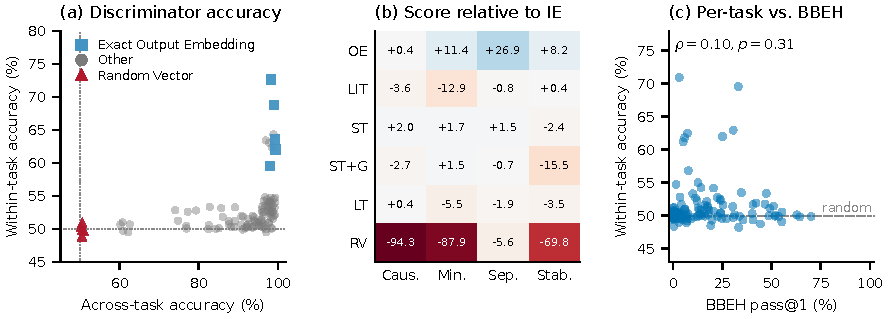
\includegraphics[width=\linewidth]{figures/pdf/results_summary.pdf}
  \caption{(a) Discriminator accuracy on across- and within-task pairs, one point per (LLM, candidate). (b) Per-axiom score relative to the Input Embedding reference, family-best per LLM averaged across LLMs. (c) Per-task within-task accuracy versus BBEH pass@$1$ (per-LLM detail in \cref{appendix:downstream}).}
  \label{fig:results_summary}
\end{figure}


% Auto-generated by scripts/tables/headline_tables.py.
% Family-best per source LLM. Cells are shaded by the |z|-score of
% the bootstrap-paired gap to IE (blue: above IE, red: below); the
% raw $\pm$SE is not rendered to keep the wraptable narrow. Edit the
% script, not this file.

\begin{table}[t]
\vspace{-1.0\baselineskip}
  \centering
  \scriptsize
  \setlength{\tabcolsep}{2.5pt}
  \renewcommand{\arraystretch}{1.05}
  \begin{tabular}{@{}l ccccccc@{}}
    \toprule
    \textbf{LLM} & OE & LIT & ST & STN & LT & IE & RV \\
    \midrule
    Llama 8B    & \cellcolor{okabeBlue!10}$0.96$ & $0.94$ & $0.94$ & \cellcolor{okabeOrange!10}$0.90$ & $0.92$ & $0.93$ & \cellcolor{okabeOrange!35}$0.52$ \\
    Llama 70B   & \cellcolor{okabeOrange!19}$0.89$ & \cellcolor{okabeOrange!10}$0.89$ & \cellcolor{okabeOrange!27}$0.85$ & \cellcolor{okabeOrange!27}$0.84$ & \cellcolor{okabeOrange!19}$0.87$ & $0.92$ & \cellcolor{okabeOrange!35}$0.50$ \\
    DS-R1 32B   & \cellcolor{okabeBlue!19}$0.96$ & \cellcolor{okabeBlue!10}$0.95$ & \cellcolor{okabeBlue!10}$0.95$ & \cellcolor{okabeOrange!27}$0.85$ & \cellcolor{okabeOrange!10}$0.92$ & $0.94$ & \cellcolor{okabeOrange!35}$0.50$ \\
    Sky-OR1 32B & \cellcolor{okabeBlue!27}$0.97$ & \cellcolor{okabeBlue!10}$0.96$ & \cellcolor{okabeBlue!10}$0.95$ & \cellcolor{okabeOrange!27}$0.86$ & $0.92$ & $0.93$ & \cellcolor{okabeOrange!35}$0.49$ \\
    GPT-OSS 20B & \cellcolor{okabeBlue!10}$0.74$ & $0.58$ & $0.55$ & \cellcolor{okabeOrange!10}$0.46$ & $0.59$ & $0.59$ & $0.56$ \\
    \bottomrule
  \end{tabular}
  \vspace{-1.0\baselineskip}

\caption{DCS AUROC ($\uparrow$, $\tau{=}0.9$).}
\label{tab:stability-headline}
\end{table}

\textbf{Stability.} The DCS is the AUROC of a probe that predicts from the candidate whether a question's beam outputs span more than one semantic equivalence class (\cref{tab:stability-headline}). On the four LLMs that produce non-singleton beam clusters on a sizeable fraction of questions, the candidates clear the Random Vector baseline by a wide margin, the Output Embedding family ranks highest, and the iterative thinking families exhibit decreasing DCS as the step count grows, with the largest decrease for Latent Thinking. The Input Embedding reference matches or exceeds the iterative candidates and is the highest-scoring representation on Llama-70B, reflecting that distributional uncertainty is largely predictable from the question text alone. GPT-OSS-20B is an MoE outlier whose forced beam-generation protocol yields almost no divergent semantic outputs across questions, leaving the DCS estimates uninformative rather than indicative of DCS failure. Per-variant tables across all candidates and step counts, the per-step DCS trajectory, and the projection- and length-control ablations are reported in \cref{appendix:sub:detailed_results,appendix:causality_length,appendix:sub:causality_minproj,appendix:sub:dcs_tau,appendix:capacity_ablation,appendix:sub:minimality_ib_derivation}.

\subsection{Per-family analysis}
\label{sec:results:per-family}

\textbf{Output Embedding as anchor.} The Output Embedding family serves as the upper anchor on axes that reward information about the generated continuation, since these candidates are computed from the output directly. On Causality and Separability the Output Embedding is near the maximum achievable score on every source LLM. In the within-task discrimination setting it is the only family exceeding the random baseline by a meaningful margin, with the Exact variant above the Pooled variant. The Output Embedding is not a meaningful Minimality reference, as its construction violates the chain-rule simplification that the Minimality decomposition assumes. \Cref{appendix:geometric} traces this advantage reaching content related to the  question encoded along the Output Embedding directions that other candidates sharing its cluster coordinates do not carry.

\textbf{Cross-axis pattern.} \Cref{fig:results_summary}(b) reports the per-axiom score of each family relative to the Input Embedding reference, averaged across LLMs and computed from the family-best variant per (LLM, axis) pair, with a Random Vector row as a sanity-check anchor. The heatmap recovers the Separability collapse from \cref{sec:results:per-axiom} and exposes three additional patterns. On within-task Separability, only the Output Embedding clears the random baseline. On Minimality, the iterative thinking families are mostly above the Input Embedding reference whereas Last Input Token is below it, since Last Input Token encodes input-specific information that is not used in the explicit output but is intrinsic to the input. On Stability, the iterative families and Last Input Token are close to the reference, with Soft Thinking with Gumbel noise as the only outlier. The decrease after adding noise is expected and reinforces why noise is a critical step for exploration~\citep{deng2025latentreasoningllmsvocabularyspace, wu2026llms}.

The Output Embedding's Causality cell is within bootstrap noise of the Input Embedding reference, reflecting a substantive empirical observation rather than a normalization artifact. Output Embedding and Input Embedding project into regions of the model's space that perturb the continuation distribution by comparable amounts, leaving neither dominant on this axis. Taken together, no iterative thinking family achieves the simultaneous strong clustering, wide within-task spread, and high within-question similarity that the framework rewards. The per-family geometric trajectories and the uniform failure pattern across architectures and sizes are reported in \cref{appendix:geometric}.

\subsection{Joint behavior and synthesis}
\label{sec:results:joint}
% Per-LLM consistency table (wrapped). For each candidate
% configuration, count the (axis, source LLM) cells out of 20
% (4 axes x 5 LLMs) on which it beats the Input Embedding reference.
\begin{table}[t]
\vspace{-0.6em}
  \centering
  \footnotesize
  \setlength{\tabcolsep}{3pt}
  \renewcommand{\arraystretch}{1.05}
  \definecolor{c4low}{HTML}{F4D8C8}
  \definecolor{c4high}{HTML}{D6E8F4}
  \begin{tabular}{@{}l c@{}}
    \toprule
    \textbf{Candidate} & \textbf{Cells/$20$} \\
    \midrule
    Exact                & \cellcolor{c4high}$16$ \\
    Pooled               & \cellcolor{c4high}$16$ \\
    LIT (all, final)     & \cellcolor{c4low}$6$ \\
    \midrule
    ST@$1$               & $13$ \\
    ST@$16{-}128$        & \cellcolor{c4low}$3{-}5$ \\
    STN@$1$              & $7$ \\
    STN@$16{-}128$       & \cellcolor{c4low}$2{-}3$ \\
    LT@$1$               & $7$ \\
    LT@$16{-}128$        & \cellcolor{c4low}$2{-}3$ \\
    \bottomrule
  \end{tabular}
  \vspace{-0.6em}

\caption{Cells beating IE.}
\label{tab:per-llm-consistency}
\end{table}

No candidate thought representation consistently exceeds the Input Embedding reference on any of the four axes when results are averaged across LLMs. The per-LLM advantages reported by \cref{tab:causality-headline,tab:minimality-headline,tab:separability-headline,tab:stability-headline} for individual candidates do not generalize (\cref{tab:per-llm-consistency}). In addition, the evaluation does not match what benchmark accuracy alone would predict. A model can score well on a reasoning benchmark while its thought representations fail to discriminate two questions drawn from the same task. The per-task correlation between Separability and downstream accuracy in panel (c) of \cref{fig:results_summary} confirms that this collapse is not explained by task difficulty. The framework's contribution is a measurement protocol that exposes these gaps at the representation level, without retraining the source model and without dependence on a downstream benchmark.

\textbf{Takeaway.} \textit{No candidate beats the Input Embedding reference on every axis across the tested LLMs, and the iterative thinking variants degrade as the step count grows.}

\FloatBarrier

\section{Conclusion}
\label{conclusion}

We introduce an axiomatic evaluation framework for candidate thought representations that runs directly on the source LLM without retraining, instantiated by four measures. We apply this methodology across LLMs that span dense, sparse-MoE, reasoning-distilled, and RL-trained paradigms. The protocol exposes a representational collapse on per-question identity that downstream task accuracy does not reveal. By focusing our evaluation on the representation rather than the subsequent reasoning process, our approach provides a unified foundation. This principled approach readily adapts to new thought representations and axiom measurement designs. Future contributions can propose additional candidate constructions beyond the soft-thinking, latent-thinking, and hidden-state families considered in this work.

\textbf{Implications.} The four axioms serve as explicit optimization targets and diagnostic readouts for thought representations. A new candidate can be scored on each axiom independently, so any change in downstream reasoning accuracy is attributable to the property responsible rather than to an aggregate benchmark score that obscures the cause. An audit identifies which axiom is the binding constraint on an existing representation before any retraining is undertaken, and competing representations are compared directly on a four-metric profile rather than on a single accuracy number. This places future thought representation development on explicit, decomposable, and directly comparable properties that researchers can utilize.

\textbf{Limitations.}
The lexical invariance sub-property of Stability is not measured
because every candidate evaluated here produces vectors identical
across paraphrases by construction, leaving the sub-property trivial
in our setting. A measurement protocol awaits candidate constructions
that admit non-trivial paraphrase variation. Measurement cost
exceeds that of running a single accuracy benchmark, as the protocol
requires LLM generations and an additional short probe training
step. We position the framework as orthogonal to reasoning benchmark evaluation,
where the cost of running the protocol once is small relative to the
representation quality information it produces. The empirical audit covers
the 23 reasoning tasks of BBEH and five open-weight English-language LLMs
spanning a range of architectures, sizes, and training paradigms, and our
conclusions do not necessarily hold for multilingual workloads or for
generations outside reasoning. Finally, the candidates audited here are
all obtainable from a pre-trained LLM without any additional training, and
representations satisfying all four axioms may require specifically designed extraction that is trained explicitly to meet those functional requirements.
Applying the protocol to such representations is a natural direction for
future work.



\bibliographystyle{abbrvnat}
\bibliography{references}


\appendix
\appendix

\etocdepthtag.toc{appendix}

\etocsettagdepth{main}{none}
\etocsettagdepth{appendix}{subsection}
\etocsettocstyle{\section*{\centering Appendix Table of Contents}}{\bigskip}
\tableofcontents

\section{Extended Related Work}
\label{appendix:extended_related_work}

\textbf{Surveys and theoretical analyses.}
A growing set of surveys systematically categorises the emerging space of latent and continuous reasoning methods. \citet{chen2025reasoninglanguagecomprehensivesurvey} provide a comprehensive taxonomy organising approaches along two axes: token-wise horizontal methods that replace discrete tokens with continuous counterparts, and layer-wise vertical methods that propagate latent state across transformer depth. \citet{zou2026the} offer a theoretical characterisation of the fundamental exploration--execution trade-off between discrete and continuous reasoning, proving that discrete chain-of-thought is forced into a high-certainty regime while continuous representations enable exploration at the cost of amplified noise on computational tasks; they introduce the Symbolic Index as a scalar measure of decisional certainty that governs this trade-off. \citet{mondorf2024accuracyevaluatingreasoningbehavior} survey evaluation practices for reasoning in LLMs, arguing that downstream accuracy conflates reasoning quality with surface-level pattern matching. \citet{sui2025stopoverthinkingsurveyefficient} and \citet{feng2025efficientreasoningmodelssurvey} survey efficient reasoning from the angle of compute cost and length budgets. Together these works catalogue methods and their downstream trade-offs, whereas our framework evaluates the intrinsic representational quality of the intermediate state independently of the decoding strategy or task accuracy.

\textbf{Latent world models, monitoring, and localization.}
Beyond reasoning benchmarks, a parallel line of work demonstrates that LLMs build structured internal models of the world as they process language. \citet{feng2025monitoring} show that latent world states can be extracted as structured propositions via propositional probes, providing direct empirical grounding for our Separability axiom: the hidden states must contain linearly decodable information about the semantic state of the world. \citet{Du_2025} find that human-like object concept representations emerge naturally in multimodal LLMs without explicit supervision, consistent with the view that the internal geometry supports rich semantic structure. Localizing where this structure resides has received substantial attention. \citet{bandarkar2025layerswappingzeroshotcrosslingual} show that swapping transformer layer ranges transfers cross-lingual knowledge across models, and \citet{alabi-etal-2024-hidden} find that adaptation concentrates in early-to-middle adapter layers, both implying semantically meaningful computations are localized at identifiable depths. \citet{sun2025transformerlayerspainters} show that middle layers can be reordered or skipped with minimal accuracy cost, consistent with mid-depth representations sharing structural properties across depth. \citet{ameisen2025circuit} trace computational circuits through residual stream contributions and demonstrate that feature-level computations shift dynamically across layers depending on the prompt, directly motivating why a fixed layer selection strategy for thought representation extraction is insufficient and why our framework tests multiple candidate extraction points.

\textbf{Sentence-level and continuous-space representations.}
A separate family of methods pursues meaning representation at the sentence level rather than the token level. Large Concept Models~\citep{lcm2024} reformulate language modelling as prediction in a sentence embedding space rather than over token vocabularies, leveraging SONAR~\citep{duquenne2023sonarsentencelevelmultimodallanguageagnostic} as the shared multilingual sentence encoder. SONAR-LLM~\citep{dragunov2025sonarllm} extends this further with an autoregressive transformer that reasons in sentence embedding space and decodes back to tokens, operating at a granularity coarser than individual tokens but finer than document-level representations. These methods design representations at a fixed semantic granularity chosen a priori. Our framework is granularity-agnostic and instead asks whether representations produced at any granularity by an existing model satisfy the four axioms, making it applicable to sentence-level methods as a diagnostic tool as well as to the token-level iterative candidates we evaluate here.

\section{Formal Analysis of the Axiomatic System}
\label{appendix:theoretical_properties}

In this section, we provide the theoretical justification for the four axiomatic properties defined in Section \ref{methodology}. We use the same notation as the main text. Appendix-specific symbols are introduced where they first appear. We formally establish the logical framework of the set $\mathcal{P} = \{\text{Causality}, \text{Minimality}, \text{Separability}, \text{Stability}\}$.

\subsection{Consistency (Existence)}
\label{app:consistency}

We first analyze the logical consistency of $\mathcal{P}$. In empirical, frozen language models trained via next-token prediction, there exists an inherent tension between Causality (which requires $\mathbf{T}$ to perfectly mimic the lexically-entangled predictive state of $\mathcal{M}_\theta$) and Stability/Minimality (which require $\mathbf{T}$ to discard lexical information). 

\begin{proposition}
The set of properties $\mathcal{P}$ is logically consistent. There exists an idealized model configuration $\mathcal{M}^*$ and representation $\mathbf{T}^*$ that satisfies all four axioms simultaneously.
\end{proposition}

\begin{proof}
To prove strict logical consistency, we construct an idealized model $\mathcal{M}^*$ whose intermediate representations perfectly disentangle semantics from syntax.
Let $\mathcal{S}_{\mathcal{M}}$ be a discrete semantic space. Let $\mathcal{M}^*$ be constructed such that its forward pass strictly factors through a one-hot semantic bottleneck before projecting to vocabulary logits, a construction closely related to the discrete latent bottlenecks used in recent latent reasoning architectures~\citep{deng2025latentreasoningllmsvocabularyspace}. Let $\mathbf{T}^*$ be the one-hot activation at this bottleneck.
\begin{enumerate}
    \item \textbf{Causality:} Because $\mathcal{M}^*$ explicitly generates $Z$ conditioned entirely on this semantic bottleneck, substituting the explicit sequence $Y$ with $\mathbf{T}^*$ yields identical downstream logits, so $D_{\text{KL}}(P_{\mathcal{M}^*}(Z \mid Y) \parallel P_{\mathcal{M}^*}(Z \mid \mathbf{T}^*)) = 0$, matching the formal causality criterion of \cref{methodology}.
    \item \textbf{Minimality:} By construction $Y$ depends on $X$ only through $\mathbf{T}^*$, so $X \to \mathbf{T}^* \to Y$ forms a Markov chain and $\mathbf{T}^*$ is sufficient with $I(\mathbf{T}^*; Y) = I(X; Y)$. For any deterministic sufficient statistic $T = T(X)$, $I(X; T) = H(T) \geq I(T; Y) = I(X; Y)$, with equality precisely when $T$ is a bijective function of $\mathbf{T}^*$. Hence $\mathbf{T}^*$ attains the minimum of $I(X; T)$ over all sufficient $T$ and saturates the information-bottleneck objective. This is an existence claim about the idealized configuration $\mathcal{M}^*$. The empirical question of how closely a given frozen $\mathcal{M}_\theta$ approaches this construction is what \cref{sec:results} measures.
    \item \textbf{Separability:} Distinct semantic intents map to orthogonal one-hot vectors, perfectly resolvable by any linear projection $\phi \in \mathcal{H}$.
    \item \textbf{Stability:} Semantically equivalent outputs map deterministically to the same one-hot bottleneck, ensuring perfect lexical invariance at the output level. Mode Collapse Resistance holds vacuously in $\mathcal{M}^*$: by construction, each input $x$ induces a deterministic semantic class, so $P(Y \mid x)$ is a point mass with $H_x = 0$. There is no distributional uncertainty to represent or collapse, and the one-hot encoding faithfully reflects this zero-entropy output distribution.
\end{enumerate}
Because this configuration satisfies $\mathcal{P}$ without contradiction, the system is logically consistent.
\end{proof}

\begin{remark}
For an arbitrary frozen model $\mathcal{M}_\theta$ with lexical-semantic entanglement, the four axioms define a Pareto-optimal frontier rather than a strict intersection. In empirical settings $\mathbf{T}$ acts as an $\epsilon$-optimal approximation that bounds the tradeoff between causal exactness and semantic stability, consistent with prior evidence that intermediate layers balance information compression against signal preservation~\citep{skean2025layerlayeruncoveringhidden,shani2025tokensthoughtsllmshumans}. We quantify this frontier empirically in \cref{sec:results}.
\end{remark}

\subsection{Independence (Non-Redundancy)}
\label{app:independence}

\begin{proposition}
The axioms in $\mathcal{P}$ are logically independent. No property can be derived solely from the conjunction of the others.
\end{proposition}

\begin{proof}
We prove independence by constructing a theoretical counter-model for each property $p \in \mathcal{P}$ that satisfies $\mathcal{P} \setminus \{p\}$ but violates $p$. Let $\mathbf{T}^*$ be an optimal representation satisfying all axioms in an idealized network.

\paragraph{Case 1: Violation of Causality.}
Construct $\mathbf{T} = \pi(\mathbf{T}^*)$, where $\pi$ is a fixed, random permutation of the coordinate dimensions of $\mathbf{T}^*$. Throughout this case the generation head of $\mathcal{M}^*$ is held frozen, while the Separability probe $\phi \in \mathcal{H}$ may be re-fit on the new representation. This asymmetry reflects how each axiom is operationalised in \cref{methodology} (probes test latent geometry and are trained per representation, whereas Causality tests substitution into a fixed model whose head is never retrained).
\begin{itemize}
    \item \textbf{Satisfies Minimality:} A permutation is a bijection on coordinates, so $I(X; \mathbf{T}) = I(X; \pi(\mathbf{T}^*)) = I(X; \mathbf{T}^*)$ (mutual information is invariant under invertible deterministic transformations), and the information-bottleneck objective is preserved exactly.
    \item \textbf{Satisfies Separability:} Permutations are orthogonal transformations and preserve inner products. Since the Separability probe $\phi \in \mathcal{H}$ is trained on whichever representation is presented, it can absorb $\pi^{-1}$ in its first linear layer at no cost in norm or expressive power, recovering the separability of $\mathbf{T}^*$.
    \item \textbf{Satisfies Stability:} The permutation is deterministic and depends only on coordinate indices, not on the output, so $\mathbf{T}^*_{y_1} = \mathbf{T}^*_{y_2} \implies \pi(\mathbf{T}^*_{y_1}) = \pi(\mathbf{T}^*_{y_2})$, preserving lexical invariance.
    \item \textbf{Violates Causality:} The frozen generation head expects specific semantic features at specific indices. Because the head is not retrained, it cannot absorb $\pi^{-1}$, so the permuted representation activates wrong indices and is decoded as a different (typically incorrect) semantic class. Consequently $P_{\mathcal{M}^*}(Z \mid \mathbf{T})$ diverges from $P_{\mathcal{M}^*}(Z \mid Y)$ and the Causality KL spikes despite the geometry being preserved.
\end{itemize}

\paragraph{Case 2: Violation of Minimality.}
Construct $\mathbf{T} = [\mathbf{T}^*, \xi(X)]$, where $\xi(X)$ is a high-entropy nuisance vector (e.g., a hash of the exact character sequence of $X$) that is independent of the semantic class. We assume the downstream generation head structurally ignores the dimensions of $\xi(X)$ (e.g., via an attention mask that zeroes them out), so that nuisance information is appended without affecting prediction.
\begin{itemize}
    \item \textbf{Satisfies Causality:} Since the head ignores $\xi(X)$, the conditional distribution $P_{\mathcal{M}^*}(Z \mid \mathbf{T})$ depends only on the $\mathbf{T}^*$ component and matches $P_{\mathcal{M}^*}(Z \mid \mathbf{T}^*) = P_{\mathcal{M}^*}(Z \mid Y)$ exactly.
    \item \textbf{Satisfies Separability:} A linear classifier in $\mathcal{H}$ can place zero weight on the $\xi(X)$ coordinates and recover the same decision boundary as on $\mathbf{T}^*$, so the Separability margin $\delta$ is preserved.
    \item \textbf{Satisfies Stability:} Stability requires lexical invariance among sibling outputs drawn from the same input $x$. Because $\xi$ is a function of the input alone, all sibling outputs $y_i \sim_{sem} y_j$ generated from the same $x$ inherit an identical $\xi(x)$, so their representations agree.
    \item \textbf{Violates Minimality:} Independence of $\xi(X)$ from $\mathbf{T}^*$ gives $I(X; \mathbf{T}) = I(X; \mathbf{T}^*) + H(\xi(X) \mid \mathbf{T}^*) = I(X; \mathbf{T}^*) + H(\xi(X))$, so $I(X; \mathbf{T})$ exceeds the bottleneck minimum by $\Theta(H(\xi(X)))$ bits, which can be made arbitrarily large by lengthening the hash. The representation therefore carries strictly more information about $X$ than any sufficient statistic.
\end{itemize}

\paragraph{Case 3: Violation of Separability.}
\emph{Scope of $\mathcal{H}$ for this case.} The Independence argument below analyzes Separability under the trainable component of $\mathcal{H}$ and treats the frozen LLM in the empirical realization of $f_\mathrm{disc}$ (\cref{appendix:sub:disc_arch}) as a fixed feature kernel outside the optimized class. This scoping aligns with the linear representation hypothesis~\citep{park2024linear}, under which high-level semantic concepts are linearly decodable from frozen LLM activations. Because empirical $f_\mathrm{disc}$ has access to LLM-induced nonlinear features that the theoretical $\mathcal{H}$ does not, the empirical test is more permissive. An empirical Separability failure implies a theoretical violation under $\mathcal{H}$, but the converse does not hold. The construction below therefore establishes Independence at the theoretical level and a conservative refinement at the empirical level.

Fix two semantic classes $s \in \{0, 1\}$. Encode the representations such that class $0$ maps to $R_0 = \{(0,0,\mathbf{0}), (1,1,\mathbf{0})\} \subset \{0,1\}^d$ and class $1$ maps to $R_1 = \{(0,1,\mathbf{0}), (1,0,\mathbf{0})\}$, where $\mathbf{0}$ is the zero vector in $\{0,1\}^{d-2}$. The four vertices are the XOR configuration of the unit square padded into the ambient $d$-cube. The deep layers of $\mathcal{M}^*$ are parameterized to compute the XOR of the first two coordinates before decoding.
\begin{itemize}
    \item \textbf{Satisfies Causality:} The deep network applies the parity function before generation, so $\mathbf{T}$ matches the intermediate distribution the deep head expects and $P_{\mathcal{M}^*}(Z \mid \mathbf{T}) = P_{\mathcal{M}^*}(Z \mid Y)$.
    \item \textbf{Approximately satisfies Minimality:} The representation occupies four configurations for two classes, contributing a fixed overhead of one bit above the minimum-sufficient encoding of the binary class label. This is a constant, content-independent cost: $I(X; \mathbf{T}) = I(X; \mathbf{T}^*) + 1\,\text{bit}$, where the extra bit encodes within-class position but carries no additional information about $X$ beyond the class label. The violation of strict Minimality is bounded and does not grow with the semantic complexity of $X$; for the purposes of the independence argument, this $\epsilon$-deviation from strict Minimality is the same approximation acknowledged in the Remark following \cref{app:consistency}.
    \item \textbf{Satisfies Stability:} Within-class pairs satisfy $\mathbf{E}_{ij} = 1$ in the DCS equivalence matrix (\cref{methodology}) and the corresponding latent representations differ by Hamming distance at most two. The operational $\approx$ tolerance the Stability axiom permits is therefore satisfied.
    \item \textbf{Violates Separability:} The bounded hypothesis class $\mathcal{H}$ defined in \cref{methodology} consists of a linear projection into an embedding space followed by a linear head~\citep{park2024linear}. The composition of two linear maps is itself linear, so every $\phi \in \mathcal{H}$ realises a single halfspace decision $\mathrm{sign}(w^\top \mathbf{T} + b)$ over $\mathbf{T}$. We show no such halfspace separates $R_0$ from $R_1$. Requiring positive decisions on $R_0$ forces $b > 0$ and $w_1 + w_2 + b > 0$, while requiring negative decisions on $R_1$ forces $w_1 + b < 0$ and $w_2 + b < 0$. Summing the last two yields $w_1 + w_2 < -2b$, which contradicts $w_1 + w_2 + b > 0$ whenever $b > 0$. The classes are XOR-configured and provably outside the linear hypothesis class. Beyond non-realizability, gradient-based training of any such $\phi$ on parity targets needs sample complexity scaling as $\Omega(d^2)$ before any nontrivial correlation emerges~\citep{barak2022hidden}, so even the relaxed empirical version of Separability fails. No $\phi \in \mathcal{H}$ therefore attains the required margin $\delta$.
\end{itemize}

\paragraph{Case 4: Violation of Stability.}
Under \cref{def:thought-mapping}, $g$ is a deterministic function of $x$ alone, which means every beam drawn from the same input shares the same representation and Lexical Invariance is satisfied trivially. To show that Stability is not logically entailed by the remaining three axioms, we therefore work in the natural extended domain where the generator may depend on the generation trajectory: $g: \mathcal{X} \times \mathcal{Y} \to \mathcal{T}$. This extension captures stochastic extraction methods (e.g., beam-specific random seeds) and allows Lexical Invariance to be a nontrivial requirement. The independence argument below shows that even in this richer domain the other three axioms do not force Lexical Invariance. $\mathbf{T}_y$ denotes the representation value associated with output $y$ in this counter-model; $\mathbf{T}^*$ remains the input-determined component from \cref{def:thought-mapping}, and $\alpha_\mathrm{lex}(y)$ is the output-dependent augmentation whose role this case isolates.

Construct $\mathbf{T}_y = [\mathbf{T}^*, \alpha_{lex}(y)]$, where $\alpha_{lex}(y) \in \{0, \lambda\}$ is a single massive scalar that flags a trivial lexical feature of the output sequence $y$, for concreteness the presence of a trailing space. We assume the downstream generation head structurally drops this augmented index. This assumption isolates Stability cleanly. Causality, Minimality, and Separability are all preserved precisely because the offending coordinate is suppressed at inference. The case is informative for representations consumed by models without such suppression which is exactly the empirical setting we evaluate, where the frozen LLM has no architectural mechanism to know which coordinate carries lexical noise. Under those conditions, even a single uncontrolled lexical-flag dimension destroys output-level invariance.
\begin{itemize}
    \item \textbf{Satisfies Causality:} The augmented index is dropped prior to prediction, so the causal logits remain identical to those of $\mathbf{T}^*$.
    \item \textbf{Satisfies Minimality:} By construction $Y \perp X \mid \mathbf{T}^*$, so $\alpha_\mathrm{lex}(Y) \perp X \mid \mathbf{T}^*$ and $I(X; \mathbf{T}) = I(X; \mathbf{T}^*)$ exactly. Minimality is preserved without overhead.
    \item \textbf{Satisfies Separability:} Any $\phi \in \mathcal{H}$ can place zero weight on the augmented coordinate and recover the same decision boundary as on $\mathbf{T}^*$, so the Separability margin $\delta$ is preserved.
    \item \textbf{Violates Stability:} Two semantically equivalent outputs $y_i \sim_{sem} y_j$ that differ only in whether they end in a trailing space acquire $\alpha_{lex}(y_i) \neq \alpha_{lex}(y_j)$. Their representations are then separated by Euclidean distance $\lambda$, which can be made arbitrarily large, fundamentally destroying the output-level lexical invariance the axiom requires.
\end{itemize}

Therefore, no axiom logically entails another.
\end{proof}

\subsection{Completeness (Sufficiency)}
\label{app:completeness}

\begin{proposition}
The set of properties $\mathcal{P}$ is complete with respect to the definition of a Functional Thought Representation. Any representation $\mathbf{T}$ strictly satisfying $\mathcal{P}$ establishes a well-defined functional isomorphism between the reachable latent space $\mathcal{T}$ and the reachable semantic manifold $\mathcal{S}_{\mathcal{M}}$.
\end{proposition}

\begin{proof}
For each semantic class $s \in \mathcal{S}_{\mathcal{M}}$, choose a high-probability output $y \in \mathcal{Y}$ with $\Phi(y) = s$, and define $\psi : \mathcal{S}_{\mathcal{M}} \to \mathcal{T}$ by $\psi(s) = \mathbf{T}_y$. We verify that $\psi$ is a bijection onto $\mathcal{T}$.
\begin{enumerate}
    \item \textbf{Well-Defined (Stability and Minimality):} Fix a representative $y$ with $\Phi(y) = s$ to define $\psi(s) = \mathbf{T}_y$. For any other $y'$ with $\Phi(y') = s$, we need $\mathbf{T}_{y'} = \mathbf{T}_y$. If $y'$ is a sibling output drawn from the same input $x$ as $y$, strict Stability (Lexical Invariance) gives $\mathbf{T}_{y'} = \mathbf{T}_y$ directly. If $y'$ is drawn from a different input, strict Minimality forces $\mathbf{T}$ to be a function of $s$ alone, so $\mathbf{T}_{y'} = \mathbf{T}_y$ again. Hence $\psi(s)$ is well-defined.
    \item \textbf{Injective (Separability):} For distinct classes $s_1 \neq s_2$ with disjoint high-probability semantic spaces, Separability supplies some $\phi \in \mathcal{H}$ that resolves $\psi(s_1)$ from $\psi(s_2)$ with margin $\delta > 0$. In particular $\psi(s_1) \neq \psi(s_2)$, so $\psi$ is injective.
    \item \textbf{Surjective (Minimality and the generator definition):} The reachable latent $\mathcal{T}$ is defined as the image $g(\mathcal{X})$, so every $\mathbf{T} \in \mathcal{T}$ equals $g(x)$ for some input $x$, which induces a semantic class $\Phi(\mathcal{M}(x)) \in \mathcal{S}_{\mathcal{M}}$. Minimality (in the idealized limit clarified in the Remark below) additionally forces $\mathbf{T}$ to carry no information about $X$ beyond a sufficient statistic for the semantic class, because any excess would raise $I(X; \mathbf{T})$ above the bottleneck minimum. Consequently $g(x)$ coincides with $\mathbf{T}_y$ whenever $\Phi(\mathcal{M}(x)) = \Phi(y)$, so $\mathbf{T} = \psi(\Phi(\mathcal{M}(x)))$ and $\psi$ surjects onto $\mathcal{T}$.
    \item \textbf{Functional Equivalence (Causality):} Causality upgrades the set-theoretic bijection to a functional one. Each $\mathbf{T} = \psi(s)$ substitutes for the explicit output sequence $Y$ inside $\mathcal{M}_\theta$ and induces the same downstream distribution $P_{\theta}(Z \mid \mathbf{T}) = P_{\theta}(Z \mid Y)$.
\end{enumerate}
Because $\psi$ is well-defined, injective, surjective onto $\mathcal{T}$, and functionally equivalent to the explicit generative pathway, it realizes a bijection $\mathcal{T} \cong \mathcal{S}_{\mathcal{M}}$. The four axioms therefore fully determine the structural isomorphism, and no further axiom is required.
\end{proof}

\begin{remark}
The term "completeness" here refers to adequacy of the axiom set in the categoricity sense. No additional axiom is required beyond $\mathcal{P}$ to pin down the functional isomorphism up to relabeling of semantic classes. The bijection is strict in the idealized limit where Stability holds with equality and the Separability margin is unbounded. Under the empirical $\approx$ tolerance of Stability and the finite $\delta$-margin of Separability, the bijection becomes approximate and is quantified in \cref{sec:results}.
\end{remark}
\section{Training Details}
\label{appendix:sub:train_details}

\subsection{LLM Data Generation}
The generator models, benchmark, beam count, and maximum generation length
are defined in \cref{sec:exp_setup}; all models are loaded in their native precision (bfloat16). From each beam we extract hidden states at every decoding step
across all layers, and take the last token of the prefill step as the
primary thought representation (position $-1$, decoding step $0$, all
layers). The per-model layer count is 33, 81, 65, 65, and 25 for
Llama-3.1 8B, Llama-3.3 70B, DeepSeek-R1-Distill-Qwen 32B, Skywork-OR1 32B, and
GPT-OSS 20B respectively.

\subsection{Soft Thinking and Latent Thinking Generation}
\label{appendix:sub:soft_latent_formula}
Soft Thinking (No Noise) replaces discrete decoding with the
weighted combination of token embeddings $\mathbf{T} = \sum_v p_v \mathbf{e}_v$
where $p_v = \mathrm{softmax}(z)_v$ and $\mathbf{e}_v$ is the token
embedding~\citep{zhang2025softthinkingunlockingreasoning}.
Soft Thinking with Gumbel Noise applies $\hat{p}_v \propto \exp((z_v + \epsilon_v)/\tau)$
with $\epsilon_v \sim \mathrm{Gumbel}(0,1)$ and temperature
$\tau=1.0$~\citep{wu2026llms}.
Latent Thinking applies recurrent hidden state updates using
a protocol similar to COCONUT \citep{hao2024training}, as implemented in \citet{zou2025latentcollaborationmultiagentsystems}.
For all iterative methods, we evaluate steps
$s \in \{1, 16, 32, 64, 128\}$.

\paragraph{Determinism under stochastic extraction.}
The idealized mapping $g$ in \cref{def:thought-mapping} is defined deterministically. Extraction methods that include stochastic components, such as Gumbel noise in Soft Thinking, fix a global random seed across all evaluations, so each input deterministically produces the same $\mathbf{T}$. The Gumbel perturbation is therefore a property of the extraction procedure rather than a source of representational randomness, and $g$ remains well-defined as a deterministic function of $x$.

\subsection{Causality Evaluation Protocol}
\label{appendix:sub:causality_eval}
The causality evaluation does not involve training.
Given a test problem with $K=8$ beams $\{y_k\}_{k=1}^K$ and
corresponding thought representations $\{\mathbf{T}_k\}_{k=1}^K$,
we compute:
\begin{enumerate}[nosep,leftmargin=1.5em]
  \item \textbf{Prefix--suffix split}: Let $y_{\mathrm{suf}}$ denote the last 50 tokens
        of $y_k$ (the answer suffix) and $y_{\mathrm{pre}}$ the preceding tokens (the
        reasoning prefix), so that $y_k = [y_{\mathrm{pre}},\, y_{\mathrm{suf}}]$.
        Beams shorter than 51 tokens are excluded from this evaluation.
  \item \textbf{Baseline distribution}: Run the evaluation backbone on the explicit
        token embeddings of $y_{\mathrm{pre}}$ to obtain
        $P(y_{\mathrm{suf}} \mid y_{\mathrm{pre}})$ at the $y_{\mathrm{suf}}$ positions
        via teacher forcing.
  \item \textbf{Intervened distribution}: Replace the prefix embeddings
        with the projected thought representation $\mathbf{T}_k$ to
        obtain $P(y_{\mathrm{suf}} \mid \mathbf{T}_k)$ at the same positions. The
        projection is taken from an output-reconstruction projection trained on the
        source LLM's output sequences via cross-entropy loss (same training splits as
        the Minimality probe); see \cref{appendix:sub:causality_minproj}
        for the ablation comparing this choice against the discriminator projection.
        The evaluation backbone is LLaMA-3.2-1B~\citep{grattafiori2024llama3herdmodels}
        with its parameters held fixed; the projection learns to map $\mathbf{T}$ into
        the backbone's embedding space so that the KL measures whether $\mathbf{T}$
        induces the same functional generative effect on $y_{\mathrm{suf}}$ as
        $y_{\mathrm{pre}}$, rather than raw cross-model transferability.
  \item \textbf{KL divergence}: Compute
        $D_\mathrm{KL}\!\left(P(y_{\mathrm{suf}} \mid y_{\mathrm{pre}}) \,\|\,
        P(y_{\mathrm{suf}} \mid \mathbf{T}_k)\right)$
        averaged over $y_{\mathrm{suf}}$ positions.
\end{enumerate}
\paragraph{Position indices under tiling.}
Because all candidates are tiled to the same substitution length ($128$ positions), the absolute position indices seen by $y_{\mathrm{suf}}$ under LLaMA-3.2-1B's Rotary Position Embeddings are identical across every candidate for a given problem. Any KL inflation arising from the difference between the tiled length and the natural prefix length $|y_{\mathrm{pre}}|$ is therefore a constant offset shared by every candidate and does not affect their relative ordering.
This is performed on the held-out test split (\cref{appendix:dataset}),
minus beams excluded by the length gate above.
We report the mean KL across all valid beam--problem pairs.

\subsection{Minimality Probe Architecture and Training}
Two probes are trained under the same architecture, an output-reconstruction probe
estimating $\mathrm{CE}(Y \mid \mathbf{T})$ and a conditional input probe
estimating $\mathrm{CE}(X \mid Y, \mathbf{T})$.
Both probes tile $\mathbf{T}$ to 128 positions.
The probe maps $\mathbf{T}$ through a parameter-free LayerNorm, a learned linear
projection ($d_{\mathrm{thought}} \to 2048$), a second LayerNorm, and a learned
position-independent offset before prepending the result to the token embedding
sequence of the target or conditioning text, which is processed by the frozen backbone.
Training uses AdamW with a cosine learning-rate schedule
($\mathrm{lr}_{\max} = 5 \times 10^{-5}$, 1 epoch, warmup steps $= 20$),
batch size 64, and cross-entropy loss over the tokenized target sequence.

\subsection{Discriminator Architecture and Training}
\label{appendix:sub:disc_arch}
The discriminator $f_\mathrm{disc}(\mathbf{T}, Y)$ applies a parameter-free LayerNorm
to $\mathbf{T}$, projects it with a learned linear map ($d_{\mathrm{thought}} \to 2048$),
and passes the result through a second LayerNorm.
The input sequence to the frozen backbone is formed by concatenating the token embeddings
of $Y$, a learned separator embedding, the projected thought vectors, and a learned CLS
token.
The hidden state at the CLS position is classified by a two-layer head consisting of
Linear($2048 \to 1024$), LayerNorm, ReLU, Dropout($0.1$), and Linear($1024 \to 1$).
This pattern of training a binary classifier on projected latent
activations as a read-out mechanism for behavioral signals inside
transformer models is consistent with recent work on activation
read-outs across LLM families~\citep{zhan2026real}.
Training uses binary cross-entropy loss with AdamW,
learning rate $1 \times 10^{-4}$, batch size 64, and 1 epoch.

\paragraph{Hyperparameter provenance.} The probe and discriminator configurations reported in this section, including the projection dimensions, the LLaMA-3.2-1B backbone, and the optimizer settings, were selected from a small set of variants explored during initial pilots. The values listed above are fixed across every source LLM and every candidate thought representation reported in this paper. No hyperparameter was tuned on the held-out test split.

\subsection{Stability Sub-Properties and DCS Diagnostics}
\label{appendix:sub:dcs_tau}

\paragraph{Sub-property coverage.} Candidate representations fall into two empirical categories on the lexical-invariance axis. The Last Input Token, Pooled Output Embedding, Input Embedding, and Random Vector candidates, together with the iterative thinking families (Soft Thinking with and without Gumbel noise, Latent Thinking), produce a single vector per question regardless of which beam is drawn, so $\mathbf{T}_i = \mathbf{T}_j$ for every beam pair $(i,j)$ within the same question and lexical invariance holds by construction for these candidates. Mode-collapse resistance is the only Stability sub-property that admits a nontrivial test for them. The Exact Output Embedding is per-beam, with $\mathbf{T}_i = \mathrm{emb}(y_i)$ derived from each beam's generated text independently. For DCS it is aggregated per-question. Because $H_x$ is computed from pairwise cosine similarities between these same Nemotron output embeddings, the DCS score for the Exact Output Embedding confirms the alignment of the metric with the output distribution rather than a representational property under evaluation.

\paragraph{Input-embedding baseline.} We report the embedding of the question text as a question-difficulty baseline alongside all thought representations. Because $H_x$ is computed in the same embedding space, this input embedding benefits from a structural alignment with the label that model-derived representations do not share. Where it matches or exceeds thought representations, distributional uncertainty is largely predictable from the question text alone, which constitutes a finding about model capability rather than a flaw of the metric (see \cref{sec:results}).

\paragraph{GPT-OSS-20B as an MoE outlier.} GPT-OSS-20B yields a non-singleton semantic cluster across beams on only $1.0\%$ of questions at $\tau = 0.9$, against $16$--$46\%$ for the four dense source LLMs. The Random Vector baseline drifts above $0.5$ on the same model because the positive class is extremely small. The pattern is consistent with Top-$K$ MoE routing acting as a re-convergence force on diverging beams, an architectural feature absent in the four dense source LLMs that pulls beam representations back toward each other after they begin to differ. Bespoke generation techniques tailored to MoE architectures may surface divergent semantic outputs but were avoided in this audit to keep the protocol consistent across source LLMs.

\paragraph{Threshold sweep.} \Cref{fig:dcs-stability-tau} sweeps the semantic equivalence threshold $\tau$ over $\{0.70, 0.80, 0.85, 0.90, 0.95\}$ for one representative per thought-representation family across all five LLMs.
All other quantities are held fixed. Only the binarization of the cosine similarity matrix used to compute $H_x$ varies.
Rankings are stable across the full range. Families that score above the random-vector baseline at the main-text threshold do so at every other threshold, and families that score near the random baseline do so uniformly.

\citet{cencerrado2026answerneededpredictingllm} demonstrate that when $H_x$ is linearly decodable from a representation via a difference-of-means probe, the uncertainty signal is encoded within it.
We note that the converse does not necessarily follow, since a representation may encode $H_x$ through a non-linear structure that a linear probe cannot detect and would in that case score near the random baseline despite carrying the relevant information.
DCS scores near the random baseline are therefore evidence against linear encoding of distributional uncertainty rather than definitive evidence against encoding in any form.

\begin{figure}[t]
  \centering
  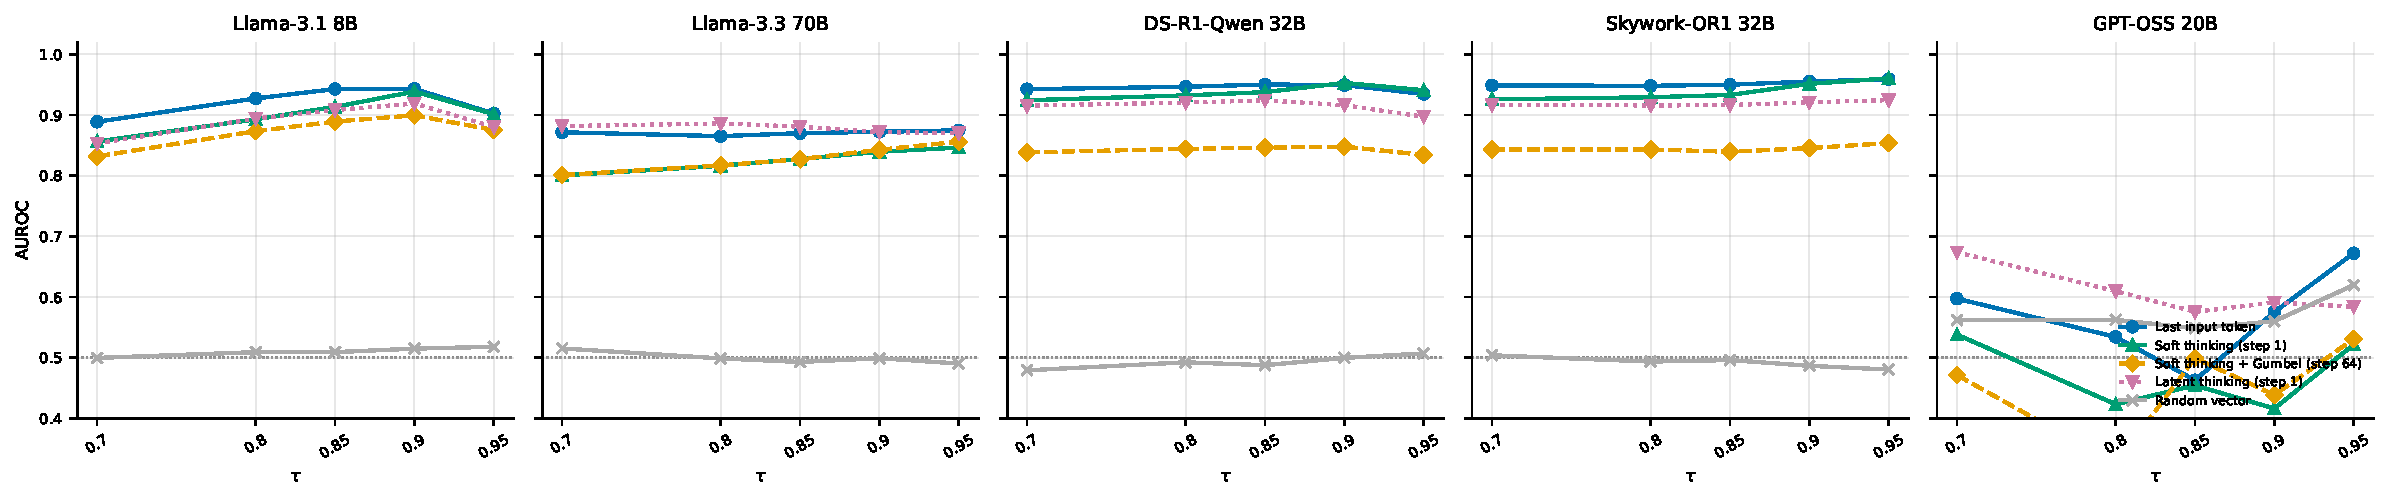
\includegraphics[width=\linewidth]{figures/pdf/dcs_stability_tau.pdf}
  \caption{DCS versus the semantic equivalence threshold $\tau$ for one representative
    per thought-representation family across all five LLMs.
    Rankings are stable across the full range shown.}
  \label{fig:dcs-stability-tau}
\end{figure}


\subsection{Reproducibility and Code Release}
\label{appendix:sub:reproducibility}

The full evaluation pipeline is publicly available at \url{https://fard-lab.github.io/formalize-thoughts} under the MIT license. The repository is organized as a Hydra project with one runnable script per phase and a shared configuration tree. Every random seed used in the pipeline is pinned in the corresponding Hydra config so that any individual phase can be re-executed without further parameter passing. Source LLMs are downloaded from public HuggingFace repositories at the identifiers given in \cref{sec:exp_setup}, BBEH is taken from the official Google DeepMind release under the Apache~2.0 license, the LLaMA-3.2-1B backbone shared by every probe and discriminator is a public HuggingFace asset, and the text embedder used is \texttt{nvidia/llama-embed-nemotron-8b} on HuggingFace.

\paragraph{Environment.} The repository targets Python~3.12 and CUDA~12.6, with dependencies pinned via \texttt{pyproject.toml} and resolved by \texttt{uv sync}. Optional flash-attention support is documented in the README and is not required to reproduce the reported numbers.

\paragraph{Hardware.} The vast majority of compute was performed on NVIDIA H100~SXM 80\,GB GPUs, including all source-LLM data generation and all discriminator training. NVIDIA A100~40\,GB GPUs were used for a small subset of probe-training and evaluation runs, without changes to the configuration.

\paragraph{Compute totals.} All numbers below are H100-equivalent GPU-hours and are reported per source LLM. LLM data generation varies substantially across tasks and source LLMs, ranging from roughly $12$ to $48$ hours per BBEH task depending on output length and model capacity, and averages near $18$ hours per task for an aggregate of approximately $400$ hours per LLM. Discriminator training comprises $42$ runs per LLM ($21$ candidates each evaluated under same-task and cross-task pairing), with each run taking roughly $3$ to $7$ hours and an aggregate of approximately $210$ hours per LLM. Minimality probe training comprises $42$ runs per LLM ($21$ candidates each producing the $\mathrm{CE}(Y\mid\mathbf{T})$ and $\mathrm{CE}(X\mid Y, \mathbf{T})$ probes that enter $\Delta_{\mathrm{IB}}$), with each run taking roughly $2$ to $4$ hours and an aggregate of approximately $125$ hours per LLM. Causality evaluation runs in roughly $15$ to $20$ minutes per candidate, for an aggregate near $6$ hours per LLM. DCS evaluation runs in roughly $5$ minutes total for all five LLMs combined, since it operates only on cached embeddings and a difference-of-means probe. Aggregating across the five source LLMs, the experiments reported in this paper consumed approximately $3{,}700$ H100-equivalent GPU-hours. The full research project consumed additional compute beyond this figure for pilot architecture and hyperparameter exploration, whose final settings underwrite the configurations recorded in \cref{appendix:sub:train_details,appendix:sub:disc_arch}.



\section{Additional Analysis}
\label{appendix:additional_analysis}

\subsection{Bootstrap Confidence Intervals}
\label{appendix:sub:bootstrap}

All main-table metrics are reported as $\mu \pm \widehat{\sigma}_B$, where
$\mu$ is the cell mean over the held-out test split and $\widehat{\sigma}_B$
is the bootstrap standard error obtained by the percentile method with
$B = 10{,}000$ resamples and a fixed random seed. The statistical
unit of resampling is the \emph{problem}, with replacement from the test split. We then recompute
the cell-level mean on the resampled problems, and take
$\widehat{\sigma}_B$ as the sample standard deviation of the resampled
means. The reported $\pm$ values are therefore $1\sigma$ bootstrap standard
errors, and a $95\%$ interval is recovered as $\mu \pm 1.96\,\widehat{\sigma}_B$
under the normal approximation, or as the $[2.5\%, 97.5\%]$ percentiles of
the bootstrap distribution when that approximation is undesirable.

The axioms differ in how each problem contributes observations, and we
resample at the problem level in every case so that within-problem
beam correlations are preserved.
\begin{itemize}[nosep,leftmargin=1.5em]
  \item \textbf{Minimality input component
        $\text{CE}(X \mid \mathbf{T})$}:
        each problem contributes one per-problem cross-entropy.
        Resample the test split; the effective sample size equals the
        test-split problem count from \cref{appendix:dataset}.
  \item \textbf{Causality} $\mathrm{KL}\!\left(P(y_{\mathrm{suf}} \mid y_{\mathrm{pre}}) \,\|\, P(y_{\mathrm{suf}} \mid \mathbf{T})\right)$:
        cluster bootstrap by problem, with all valid beams of a resampled
        problem kept together. Beams excluded by the $51$-token length
        gate are absent from the resampled mean, and problems whose
        beams are all excluded are absent entirely; on Llama-3.1-8B
        this reduces the effective support to $360$ problems. The paired
        advantage $\Delta^{\mathrm{RV}}_{\mathrm{KL}}$ is resampled on
        the same support with each $(\mathbf{T}, \mathrm{RV})$ pair kept
        glued together (see below).
  \item \textbf{Discriminator-based DCS}: the per-problem
        discriminator-based DCS score, computed over all
        off-diagonal beam pairs in the $K \times K$ within-problem matrix,
        is a single observation per problem. Resample problems, average
        per-problem score.
\end{itemize}

\paragraph{Paired advantage versus the noise floor (Causality).}
Because $\mathrm{KL}$ is unbounded above, absolute values are difficult to
compare across candidate $\mathbf{T}$ without a shared reference. We
therefore compute the paired advantage $\Delta^{\mathrm{RV}}_{\mathrm{KL}}(\mathbf{T})_g = \mathrm{KL}(\mathbf{T})_g - \mathrm{KL}(\mathrm{RV})_g$ per problem $g$, and average over the Causality support defined above.
Pairing on the problem cancels per-problem shifts in the KL scale (the
dominant source of dispersion in the raw metric), yielding a
sign-interpretable statistic where $\Delta < 0$ indicates $\mathbf{T}$ conveys
information about $y_{\mathrm{suf}}$ beyond the evaluation backbone's projection of noise,
whereas $\Delta \geq 0$ indicates no detectable advantage. The paired
bootstrap resamples problems with each
$(\mathrm{KL}(\mathbf{T})_g,\,\mathrm{KL}(\mathrm{RV})_g)$ pair kept
together, so the resulting standard error quantifies the variance of the
paired difference rather than that of the two unpaired means.
In \cref{tab:causality-results}, each cell displays the mean
$\mathrm{KL}(y_{\mathrm{suf}} \mid \mathbf{T})$ with its marginal bootstrap standard
error.

\subsection{Detailed per-axiom results}
\label{appendix:sub:detailed_results}

\Cref{tab:disc-results,tab:causality-results,tab:minimality-delta-ib}
report the cell-level mean and bootstrap standard error of the
Separability, Causality, and Minimality metrics across the populated
source LLMs. \Cref{fig:dcs-stability} reports the corresponding
Stability AUROC values. Each candidate occupies one column and each
source LLM occupies one row. The cell formatting follows the
methodology of \cref{appendix:sub:bootstrap}.

% Discriminator separability results (transposed layout).
% Rows: one LLM per block, two rows per block (Same-Task / Cross-Task).
% Columns: candidate thought representations grouped by family.
% Universal column-block explanation and bolding convention live in
% sections/experiments.tex; this caption is metric-specific only.

\begin{table}[!htbp]
  \centering
  \footnotesize
  \setlength{\tabcolsep}{1.5pt}
  \renewcommand{\arraystretch}{1.1}
  \resizebox{\textwidth}{!}{%
  \begin{tabular}{@{}l c *{2}{c} !{\vrule} *{2}{c} *{5}{c} *{5}{c} *{5}{c} !{\vrule} *{2}{c}@{}}
    \toprule
    & & \multicolumn{2}{c}{\textit{Output Emb.}}
      & \multicolumn{2}{c}{\textit{Last Input Tok.}}
      & \multicolumn{5}{c}{\textit{Soft Thinking (no noise)}}
      & \multicolumn{5}{c}{\textit{Soft Thinking (Gumbel)}}
      & \multicolumn{5}{c}{\textit{Latent Thinking}}
      & \multicolumn{2}{c}{\textit{Baselines}} \\
    \cmidrule(lr){3-4}\cmidrule(lr){5-6}\cmidrule(lr){7-11}\cmidrule(lr){12-16}\cmidrule(lr){17-21}\cmidrule(lr){22-23}
    \textbf{LLM} & \textbf{Reg.}
      & Exc & Pool
      & All & Final
      & 1 & 16 & 32 & 64 & 128
      & 1 & 16 & 32 & 64 & 128
      & 1 & 16 & 32 & 64 & 128
      & IE & RV \\
    \midrule
    \multirow{2}{*}{Llama-3.1 8B}
      & Same  & \ciSE{68.79}{0.81} & \ciSE{64.33}{0.81} & \ciSE{53.39}{0.62} & \ciSE{53.93}{0.71} & \ciSE{53.15}{0.61} & \ciSE{53.50}{0.64} & \ciSE{54.12}{0.76} & \ciSE{54.74}{0.68} & \ciSE{52.49}{0.61} & \ciSE{52.60}{0.80} & \ciSE{52.60}{0.76} & \ciSE{52.57}{0.66} & \ciSE{53.55}{0.62} & \ciSE{51.02}{0.65} & \ciSE{54.72}{0.83} & \ciSE{53.57}{0.65} & \ciSE{53.00}{0.81} & \ciSE{52.54}{0.67} & \ciSE{52.65}{0.70} & \ciSE{54.52}{0.78} & \ciSE{48.85}{0.60} \\
      & Cross & \ciSE{98.99}{0.19} & \ciSE{98.89}{0.18} & \ciSE{96.09}{0.32} & \ciSE{99.24}{0.13} & \ciSE{85.70}{0.78} & \ciSE{97.43}{0.37} & \ciSE{97.76}{0.30} & \ciSE{98.17}{0.26} & \ciSE{97.70}{0.30} & \ciSE{77.20}{0.98} & \ciSE{96.42}{0.43} & \ciSE{96.07}{0.44} & \ciSE{97.32}{0.32} & \ciSE{97.64}{0.33} & \ciSE{99.32}{0.10} & \ciSE{98.67}{0.18} & \ciSE{98.41}{0.22} & \ciSE{98.71}{0.16} & \ciSE{98.63}{0.19} & \ciSE{98.94}{0.17} & \ciSE{50.50}{0.56} \\
    \midrule
    \multirow{2}{*}{Llama-3.3 70B}
      & Same  & \ciSE{72.62}{0.77} & \ciSE{54.25}{0.52} & \ciSE{51.56}{0.45} & \ciSE{50.08}{0.28} & \ciSE{52.79}{0.66} & \ciSE{52.93}{0.49} & \ciSE{51.55}{0.33} & \ciSE{51.12}{0.58} & \ciSE{51.30}{0.46} & \ciSE{52.83}{0.49} & \ciSE{51.96}{0.45} & \ciSE{50.26}{0.42} & \ciSE{51.94}{0.51} & \ciSE{51.01}{0.35} & \ciSE{50.50}{0.33} & \ciSE{50.50}{0.28} & \ciSE{51.42}{0.47} & \ciSE{51.01}{0.48} & \ciSE{50.73}{0.34} & \ciSE{52.09}{0.54} & \ciSE{49.67}{0.61} \\
      & Cross & \ciSE{98.29}{0.24} & \ciSE{96.42}{0.27} & \ciSE{98.77}{0.14} & \ciSE{98.55}{0.16} & \ciSE{79.33}{0.72} & \ciSE{95.91}{0.41} & \ciSE{92.53}{0.53} & \ciSE{94.15}{0.52} & \ciSE{94.01}{0.46} & \ciSE{74.05}{0.81} & \ciSE{93.67}{0.56} & \ciSE{93.43}{0.50} & \ciSE{90.76}{0.66} & \ciSE{60.76}{0.92} & \ciSE{96.89}{0.25} & \ciSE{94.18}{0.37} & \ciSE{95.82}{0.29} & \ciSE{94.86}{0.34} & \ciSE{92.57}{0.39} & \ciSE{96.25}{0.30} & \ciSE{51.04}{0.60} \\
    \midrule
    \multirow{2}{*}{DS-R1-Qwen 32B}
      & Same  & \ciSE{63.54}{0.72} & \ciSE{63.05}{0.80} & \ciSE{52.13}{0.71} & \ciSE{52.56}{0.81} & \ciSE{53.26}{0.53} & \ciSE{54.45}{0.65} & \ciSE{54.81}{0.76} & \ciSE{53.86}{0.69} & \ciSE{53.42}{0.68} & \ciSE{50.69}{0.59} & \ciSE{51.84}{0.62} & \ciSE{50.90}{0.38} & \ciSE{51.33}{0.52} & \ciSE{51.06}{0.46} & \ciSE{50.33}{0.25} & \ciSE{50.06}{0.27} & \ciSE{49.94}{0.58} & \ciSE{50.21}{0.25} & \ciSE{50.22}{0.35} & \ciSE{53.53}{0.63} & \ciSE{50.28}{0.61} \\
      & Cross & \ciSE{99.18}{0.18} & \ciSE{97.79}{0.27} & \ciSEB{99.24}{0.18} & \ciSE{98.33}{0.28} & \ciSE{89.16}{0.53} & \ciSE{97.25}{0.37} & \ciSE{96.79}{0.42} & \ciSE{98.27}{0.30} & \ciSE{97.90}{0.31} & \ciSE{62.58}{1.13} & \ciSE{91.18}{0.76} & \ciSE{96.03}{0.52} & \ciSE{95.80}{0.50} & \ciSE{95.31}{0.48} & \ciSE{96.09}{0.35} & \ciSE{98.33}{0.22} & \ciSE{97.04}{0.32} & \ciSE{96.28}{0.32} & \ciSE{93.60}{0.48} & \ciSE{96.76}{0.44} & \ciSE{50.22}{0.58} \\
    \midrule
    \multirow{2}{*}{Skywork-OR1 32B}
      & Same  & \ciSE{62.04}{0.90} & \ciSE{63.41}{0.94} & \ciSE{53.26}{0.68} & \ciSE{51.94}{0.71} & \ciSE{53.32}{0.79} & \ciSE{54.19}{0.72} & \ciSE{52.82}{0.67} & \ciSE{52.25}{0.62} & \ciSE{52.64}{0.58} & \ciSE{50.65}{0.72} & \ciSE{51.76}{0.53} & \ciSE{50.58}{0.54} & \ciSE{51.74}{0.64} & \ciSE{50.91}{0.60} & \ciSE{51.23}{0.44} & \ciSE{50.28}{0.38} & \ciSE{50.22}{0.66} & \ciSE{50.12}{0.44} & \ciSE{50.06}{0.53} & \ciSE{54.01}{0.72} & \ciSE{49.85}{0.56} \\
      & Cross & \ciSE{99.41}{0.16} & \ciSE{96.93}{0.36} & \ciSE{99.14}{0.17} & \ciSE{98.95}{0.16} & \ciSE{82.78}{0.74} & \ciSE{98.16}{0.34} & \ciSE{97.57}{0.40} & \ciSE{98.11}{0.32} & \ciSE{98.09}{0.30} & \ciSE{60.20}{1.15} & \ciSE{93.94}{0.65} & \ciSE{95.31}{0.55} & \ciSE{98.16}{0.33} & \ciSE{97.72}{0.32} & \ciSE{74.75}{0.79} & \ciSE{88.97}{0.63} & \ciSE{92.24}{0.64} & \ciSE{91.62}{0.60} & \ciSE{76.92}{0.88} & \ciSE{97.82}{0.31} & \ciSE{50.51}{0.58} \\
    \midrule
    \multirow{2}{*}{GPT-OSS 20B}
      & Same  & \ciSE{59.57}{0.89} & \ciSE{62.38}{0.99} & \ciSE{50.40}{0.62} & \ciSE{50.29}{0.51} & \ciSE{50.46}{0.74} & \ciSE{50.11}{0.50} & \ciSE{50.72}{0.82} & \ciSE{49.71}{0.73} & \ciSE{50.57}{0.94} & \ciSE{49.49}{0.72} & \ciSE{50.57}{0.72} & \ciSE{51.81}{0.67} & \ciSE{51.16}{0.85} & \ciSE{49.97}{0.68} & \ciSE{51.20}{0.70} & \ciSE{50.00}{0.62} & \ciSE{50.64}{0.49} & \ciSE{50.33}{0.49} & \ciSE{49.92}{0.59} & \ciSE{49.47}{0.82} & \ciSE{50.95}{0.57} \\
      & Cross & \ciSE{97.94}{0.38} & \ciSE{98.49}{0.30} & \ciSE{95.19}{0.39} & \ciSE{88.11}{0.65} & \ciSE{76.83}{1.05} & \ciSE{85.11}{0.87} & \ciSE{87.54}{0.84} & \ciSE{60.91}{1.07} & \ciSE{92.22}{0.68} & \ciSE{62.14}{1.18} & \ciSE{82.51}{0.96} & \ciSE{86.06}{0.94} & \ciSE{87.62}{0.88} & \ciSE{82.40}{0.91} & \ciSE{89.10}{0.73} & \ciSE{84.29}{0.80} & \ciSE{90.74}{0.65} & \ciSE{92.12}{0.57} & \ciSE{91.07}{0.60} & \ciSE{97.03}{0.45} & \ciSE{50.53}{0.59} \\
    \bottomrule
  \end{tabular}%
  }
\caption{Discriminator test accuracy (\%) across source LLMs. Each LLM spans two rows, \textbf{Same} (within-task instance discrimination) and \textbf{Cross} (across-task discrimination). A uniform random classifier scores $50\%$ as data is balanced.}
\label{tab:disc-results}
\end{table}

% Headline causality. Cells display the mean KL(Z | T) with its
% marginal bootstrap SE (cluster bootstrap over problems, 10k resamples).
% Source: outputs/causality/llama8b_minproj_tiled (proj_source=minimality_output,
% tile_to_length=128).

\begin{table}[!htbp]
  \centering
  \footnotesize
  \setlength{\tabcolsep}{2.5pt}
  \renewcommand{\arraystretch}{1.1}
  \resizebox{\textwidth}{!}{%
  \begin{tabular}{@{}l *{2}{c} !{\vrule} *{2}{c} *{5}{c} *{5}{c} *{5}{c} !{\vrule} *{2}{c}@{}}
    \toprule
    & \multicolumn{2}{c}{\textit{Output Emb.}}
      & \multicolumn{2}{c}{\textit{Last Input Tok.}}
      & \multicolumn{5}{c}{\textit{Soft Thinking (no noise)}}
      & \multicolumn{5}{c}{\textit{Soft Thinking (Gumbel)}}
      & \multicolumn{5}{c}{\textit{Latent Thinking}}
      & \multicolumn{2}{c}{\textit{Baselines}} \\
    \cmidrule(lr){2-3}\cmidrule(lr){4-5}\cmidrule(lr){6-10}\cmidrule(lr){11-15}\cmidrule(lr){16-20}\cmidrule(lr){21-22}
    \textbf{LLM}
      & Exc & Pool
      & All & Final
      & 1 & 16 & 32 & 64 & 128
      & 1 & 16 & 32 & 64 & 128
      & 1 & 16 & 32 & 64 & 128
      & IE & RV \\
    \midrule
    Llama-3.1 8B     & \ciSE{5.25}{0.08} & \ciSE{5.21}{0.08} & \ciSE{5.26}{0.06} & \ciSE{5.01}{0.08} & \ciSE{5.07}{0.08} & \ciSE{5.69}{0.07} & \ciSE{5.51}{0.07} & \ciSE{5.07}{0.06} & \ciSE{4.96}{0.06} & \ciSE{5.20}{0.07} & \ciSE{5.42}{0.07} & \ciSE{5.06}{0.06} & \ciSE{4.70}{0.06} & \ciSE{4.73}{0.06} & \ciSE{5.32}{0.07} & \ciSE{5.79}{0.08} & \ciSE{6.05}{0.08} & \ciSE{6.49}{0.08} & \ciSE{6.17}{0.08} & \ciSE{5.36}{0.07} & \ciSE{9.49}{0.06} \\
    Llama-3.3 70B    & \ciSE{4.56}{0.06} & \ciSE{4.58}{0.05} & \ciSE{6.00}{0.06} & \ciSE{5.28}{0.06} & \ciSE{4.65}{0.05} & \ciSE{5.36}{0.06} & \ciSE{5.63}{0.06} & \ciSE{5.19}{0.05} & \ciSE{5.48}{0.06} & \ciSE{5.08}{0.05} & \ciSE{5.22}{0.06} & \ciSE{5.21}{0.05} & \ciSE{5.34}{0.07} & \ciSE{5.44}{0.06} & \ciSE{4.21}{0.06} & \ciSE{5.17}{0.05} & \ciSE{5.35}{0.05} & \ciSE{5.45}{0.05} & \ciSE{5.88}{0.06} & \ciSE{4.71}{0.06} & \ciSE{8.93}{0.05} \\
    DS-R1-Qwen 32B   & \ciSE{4.67}{0.06} & \ciSE{4.77}{0.07} & \ciSE{6.33}{0.07} & \ciSE{4.79}{0.07} & \ciSE{4.45}{0.07} & \ciSE{5.60}{0.08} & \ciSE{5.74}{0.07} & \ciSE{5.34}{0.07} & \ciSE{4.82}{0.06} & \ciSE{4.57}{0.07} & \ciSE{5.42}{0.06} & \ciSE{5.00}{0.06} & \ciSE{4.91}{0.06} & \ciSE{4.98}{0.06} & \ciSE{4.62}{0.07} & \ciSE{5.41}{0.07} & \ciSE{4.84}{0.07} & \ciSE{5.77}{0.07} & \ciSE{5.36}{0.07} & \ciSE{4.50}{0.07} & \ciSE{9.36}{0.05} \\
    Skywork-OR1 32B  & \ciSE{4.10}{0.06} & \ciSE{4.37}{0.06} & \ciSE{6.39}{0.06} & \ciSE{4.09}{0.06} & \ciSE{3.90}{0.06} & \ciSE{5.07}{0.06} & \ciSE{4.86}{0.05} & \ciSE{4.62}{0.05} & \ciSE{4.82}{0.05} & \ciSE{4.75}{0.07} & \ciSE{4.91}{0.05} & \ciSE{4.68}{0.05} & \ciSE{4.72}{0.05} & \ciSE{4.89}{0.05} & \ciSE{5.00}{0.06} & \ciSE{4.52}{0.07} & \ciSE{4.34}{0.07} & \ciSE{4.35}{0.06} & \ciSE{4.50}{0.07} & \ciSE{4.08}{0.06} & \ciSE{9.31}{0.05} \\
    GPT-OSS 20B      & \ciSE{3.82}{0.07} & \ciSE{4.17}{0.08} & \ciSE{5.61}{0.08} & \ciSE{4.19}{0.07} & \ciSE{4.04}{0.08} & \ciSE{4.00}{0.07} & \ciSE{4.01}{0.07} & \ciSE{4.08}{0.07} & \ciSE{4.23}{0.08} & \ciSE{4.17}{0.08} & \ciSE{4.48}{0.08} & \ciSE{4.48}{0.07} & \ciSE{4.57}{0.08} & \ciSE{4.74}{0.08} & \ciSE{3.90}{0.08} & \ciSE{5.12}{0.08} & \ciSE{4.63}{0.08} & \ciSE{4.68}{0.08} & \ciSE{4.67}{0.08} & \ciSE{3.78}{0.07} & \ciSE{9.60}{0.06} \\
    \bottomrule
  \end{tabular}%
  }
\caption{KL divergence $\mathrm{KL}(P(Z \mid Y)\,\|\,P(Z \mid \mathbf{T}))$ ($\downarrow$) across source LLMs. Lower values indicate higher predictive sufficiency of $\mathbf{T}$ for the continuation.}
\label{tab:causality-results}
\end{table}

% Headline Minimality metric $\Delta_{\text{IB}} = \text{CE}(X \mid Y, \mathbf{T}) - \text{CE}(Y \mid \mathbf{T})$,
% paired per problem (CE averaged over beams within a problem before pairing).
% Equals the IB Lagrangian at $\beta = 2$ up to a TR-independent constant.
% Derivation in \cref{appendix:sub:minimality_ib_derivation}; legacy
% $\Delta_{\text{CE}}$ proxy in \cref{appendix:minimality-components}.
% Component cross-entropies in \cref{tab:minimality-ce-y-tiled,tab:minimality-ce-xyt-tiled}.

\begin{table}[!htbp]
  \centering
  \footnotesize
  \setlength{\tabcolsep}{2.5pt}
  \renewcommand{\arraystretch}{1.1}
  \resizebox{\textwidth}{!}{%
  \begin{tabular}{@{}l *{2}{c} !{\vrule} *{2}{c} *{5}{c} *{5}{c} *{5}{c} !{\vrule} *{2}{c}@{}}
    \toprule
    & \multicolumn{2}{c}{\textit{Output Emb.}}
      & \multicolumn{2}{c}{\textit{Last Input Tok.}}
      & \multicolumn{5}{c}{\textit{Soft Thinking (no noise)}}
      & \multicolumn{5}{c}{\textit{Soft Thinking (Gumbel)}}
      & \multicolumn{5}{c}{\textit{Latent Thinking}}
      & \multicolumn{2}{c}{\textit{Baselines}} \\
    \cmidrule(lr){2-3}\cmidrule(lr){4-5}\cmidrule(lr){6-10}\cmidrule(lr){11-15}\cmidrule(lr){16-20}\cmidrule(lr){21-22}
    \textbf{LLM}
      & Exc & Pool
      & All & Final
      & 1 & 16 & 32 & 64 & 128
      & 1 & 16 & 32 & 64 & 128
      & 1 & 16 & 32 & 64 & 128
      & IE & RV \\
    \midrule
    Llama-3.1 8B     & \ciSE{0.37}{0.04} & \ciSE{0.27}{0.04} & \ciSE{0.08}{0.03} & \ciSE{0.16}{0.04} & \ciSE{0.25}{0.04} & \ciSE{0.18}{0.03} & \ciSE{0.21}{0.03} & \ciSE{0.19}{0.04} & \ciSE{0.19}{0.03} & \ciSE{0.24}{0.04} & \ciSE{0.17}{0.03} & \ciSE{0.16}{0.03} & \ciSE{0.17}{0.03} & \ciSE{0.16}{0.03} & \ciSE{0.17}{0.03} & \ciSE{0.19}{0.04} & \ciSE{0.18}{0.04} & \ciSE{0.17}{0.04} & \ciSE{0.17}{0.04} & \ciSE{0.22}{0.04} & \ciSE{-0.40}{0.06} \\
    Llama-3.3 70B    & \ciSE{-0.13}{0.04} & \ciSE{-0.20}{0.03} & \ciSE{-0.33}{0.03} & \ciSE{-0.30}{0.03} & \ciSE{-0.24}{0.03} & \ciSE{-0.27}{0.03} & \ciSE{-0.32}{0.03} & \ciSE{-0.32}{0.03} & \ciSE{-0.31}{0.03} & \ciSE{-0.24}{0.03} & \ciSE{-0.31}{0.04} & \ciSE{-0.31}{0.03} & \ciSE{-0.29}{0.03} & \ciSE{-0.32}{0.03} & \ciSE{-0.31}{0.03} & \ciSE{-0.31}{0.03} & \ciSE{-0.30}{0.03} & \ciSE{-0.33}{0.03} & \ciSE{-0.31}{0.03} & \ciSE{-0.23}{0.03} & \ciSE{-0.99}{0.05} \\
    DS-R1-Qwen 32B   & \ciSE{0.07}{0.03} & \ciSE{0.05}{0.03} & \ciSE{-0.07}{0.03} & \ciSE{-0.05}{0.03} & \ciSE{0.10}{0.04} & \ciSE{0.00}{0.04} & \ciSE{-0.02}{0.04} & \ciSE{-0.01}{0.03} & \ciSE{-0.01}{0.04} & \ciSE{0.10}{0.04} & \ciSE{0.04}{0.04} & \ciSE{0.04}{0.03} & \ciSE{0.01}{0.03} & \ciSE{0.00}{0.03} & \ciSE{0.05}{0.03} & \ciSE{0.03}{0.03} & \ciSE{0.03}{0.03} & \ciSE{0.02}{0.03} & \ciSE{0.02}{0.03} & \ciSE{0.04}{0.03} & \ciSE{-0.50}{0.05} \\
    Skywork-OR1 32B  & \ciSE{-0.16}{0.03} & \ciSE{-0.19}{0.03} & \ciSE{-0.31}{0.03} & \ciSE{-0.27}{0.03} & \ciSE{-0.13}{0.03} & \ciSE{-0.28}{0.03} & \ciSE{-0.29}{0.03} & \ciSE{-0.29}{0.03} & \ciSE{-0.27}{0.03} & \ciSE{-0.14}{0.03} & \ciSE{-0.21}{0.03} & \ciSE{-0.22}{0.03} & \ciSE{-0.23}{0.03} & \ciSE{-0.25}{0.03} & \ciSE{-0.18}{0.03} & \ciSE{-0.20}{0.03} & \ciSE{-0.21}{0.03} & \ciSE{-0.21}{0.03} & \ciSE{-0.21}{0.03} & \ciSE{-0.21}{0.03} & \ciSE{-0.59}{0.05} \\
    GPT-OSS 20B      & \ciSE{-0.26}{0.04} & \ciSE{-0.22}{0.03} & \ciSE{-0.27}{0.03} & \ciSE{-0.25}{0.03} & \ciSE{-0.21}{0.03} & \ciSE{-0.21}{0.03} & \ciSE{-0.21}{0.03} & \ciSE{-0.21}{0.03} & \ciSE{-0.21}{0.03} & \ciSE{-0.20}{0.04} & \ciSE{-0.24}{0.04} & \ciSE{-0.21}{0.03} & \ciSE{-0.24}{0.03} & \ciSE{-0.21}{0.03} & \ciSE{-0.23}{0.03} & \ciSE{-0.18}{0.03} & \ciSE{-0.17}{0.03} & \ciSE{-0.18}{0.03} & \ciSE{-0.23}{0.03} & \ciSE{-0.34}{0.04} & \ciSE{-0.30}{0.05} \\
    \bottomrule
  \end{tabular}%
  }
\caption{Minimality measure $\Delta_{\text{IB}} = \text{CE}(X \mid Y, \mathbf{T}) - \text{CE}(Y \mid \mathbf{T})$ across source LLMs, paired per problem. Larger positive values indicate a representation that is more sufficient for $Y$ and adds less $X$-information beyond $Y$.}
\label{tab:minimality-delta-ib}
\end{table}

% Tiled-length component cross-entropies entering the IB-residual
% headline metric \cref{tab:minimality-delta-ib}. Both tables feed
% \mathbf{T} to the probe at a common position count
% (tile_to_length=128 in the experiments repo) so that representations
% of different native lengths are evaluated at the same window size.
% The native-length companion of CE(Y|T) is in \cref{tab:minimality-ce-y}
% under the earlier formulation.

\begin{table}[!htbp]
  \centering
  \footnotesize
  \setlength{\tabcolsep}{2.5pt}
  \renewcommand{\arraystretch}{1.1}
  \resizebox{\textwidth}{!}{%
  \begin{tabular}{@{}l *{2}{c} !{\vrule} *{2}{c} *{5}{c} *{5}{c} *{5}{c} !{\vrule} *{2}{c}@{}}
    \toprule
    & \multicolumn{2}{c}{\textit{Output Emb.}}
      & \multicolumn{2}{c}{\textit{Last Input Tok.}}
      & \multicolumn{5}{c}{\textit{Soft Thinking (no noise)}}
      & \multicolumn{5}{c}{\textit{Soft Thinking (Gumbel)}}
      & \multicolumn{5}{c}{\textit{Latent Thinking}}
      & \multicolumn{2}{c}{\textit{Baselines}} \\
    \cmidrule(lr){2-3}\cmidrule(lr){4-5}\cmidrule(lr){6-10}\cmidrule(lr){11-15}\cmidrule(lr){16-20}\cmidrule(lr){21-22}
    \textbf{LLM}
      & Exc & Pool
      & All & Final
      & 1 & 16 & 32 & 64 & 128
      & 1 & 16 & 32 & 64 & 128
      & 1 & 16 & 32 & 64 & 128
      & IE & RV \\
    \midrule
    Llama-3.1 8B     & \ciSE{0.72}{0.03} & \ciSE{0.79}{0.02} & \ciSE{0.80}{0.02} & \ciSE{0.78}{0.02} & \ciSE{0.82}{0.03} & \ciSE{0.82}{0.02} & \ciSE{0.80}{0.02} & \ciSE{0.82}{0.02} & \ciSE{0.83}{0.03} & \ciSE{0.86}{0.03} & \ciSE{0.88}{0.03} & \ciSE{0.88}{0.03} & \ciSE{0.89}{0.02} & \ciSE{0.90}{0.03} & \ciSE{0.82}{0.02} & \ciSE{0.79}{0.02} & \ciSE{0.79}{0.02} & \ciSE{0.80}{0.02} & \ciSE{0.82}{0.02} & \ciSE{0.82}{0.03} & \ciSE{7.08}{0.08} \\
    Llama-3.3 70B    & \ciSE{1.26}{0.03} & \ciSE{1.29}{0.03} & \ciSE{1.16}{0.03} & \ciSE{1.22}{0.03} & \ciSE{1.37}{0.03} & \ciSE{1.19}{0.03} & \ciSE{1.22}{0.03} & \ciSE{1.24}{0.03} & \ciSE{1.25}{0.03} & \ciSE{1.38}{0.03} & \ciSE{1.29}{0.04} & \ciSE{1.27}{0.03} & \ciSE{1.25}{0.03} & \ciSE{1.27}{0.03} & \ciSE{1.26}{0.03} & \ciSE{1.26}{0.03} & \ciSE{1.26}{0.03} & \ciSE{1.29}{0.03} & \ciSE{1.29}{0.03} & \ciSE{1.33}{0.03} & \ciSE{7.61}{0.06} \\
    DS-R1-Qwen 32B   & \ciSE{0.82}{0.03} & \ciSE{0.83}{0.03} & \ciSE{0.76}{0.02} & \ciSE{0.80}{0.02} & \ciSE{0.81}{0.02} & \ciSE{0.81}{0.03} & \ciSE{0.81}{0.03} & \ciSE{0.81}{0.02} & \ciSE{0.81}{0.03} & \ciSE{0.85}{0.03} & \ciSE{0.85}{0.03} & \ciSE{0.84}{0.03} & \ciSE{0.83}{0.03} & \ciSE{0.83}{0.03} & \ciSE{0.81}{0.02} & \ciSE{0.81}{0.03} & \ciSE{0.81}{0.03} & \ciSE{0.81}{0.03} & \ciSE{0.81}{0.03} & \ciSE{0.85}{0.03} & \ciSE{6.90}{0.07} \\
    Skywork-OR1 32B  & \ciSE{0.96}{0.03} & \ciSE{0.97}{0.03} & \ciSE{0.89}{0.02} & \ciSE{0.94}{0.03} & \ciSE{0.95}{0.03} & \ciSE{0.97}{0.03} & \ciSE{0.94}{0.03} & \ciSE{0.95}{0.03} & \ciSE{0.95}{0.03} & \ciSE{0.97}{0.03} & \ciSE{1.00}{0.03} & \ciSE{0.97}{0.03} & \ciSE{0.97}{0.03} & \ciSE{0.96}{0.03} & \ciSE{0.95}{0.03} & \ciSE{0.93}{0.03} & \ciSE{0.93}{0.03} & \ciSE{0.93}{0.03} & \ciSE{0.94}{0.03} & \ciSE{1.02}{0.03} & \ciSE{6.77}{0.07} \\
    GPT-OSS 20B      & \ciSE{0.83}{0.03} & \ciSE{0.80}{0.03} & \ciSE{0.78}{0.03} & \ciSE{0.81}{0.03} & \ciSE{0.82}{0.03} & \ciSE{0.81}{0.03} & \ciSE{0.81}{0.03} & \ciSE{0.81}{0.03} & \ciSE{0.81}{0.03} & \ciSE{0.84}{0.03} & \ciSE{0.81}{0.03} & \ciSE{0.81}{0.03} & \ciSE{0.81}{0.03} & \ciSE{0.80}{0.03} & \ciSE{0.80}{0.03} & \ciSE{0.80}{0.03} & \ciSE{0.80}{0.03} & \ciSE{0.81}{0.03} & \ciSE{0.81}{0.03} & \ciSE{0.84}{0.03} & \ciSE{6.59}{0.08} \\
    \bottomrule
  \end{tabular}%
  }
\caption{Output-prediction cross-entropy $\text{CE}(Y \mid \mathbf{T})$ across source LLMs with $\mathbf{T}$ tiled to a common length. The tiled form is the one entering the IB-residual measure of \cref{tab:minimality-delta-ib}. Comparison with \cref{tab:minimality-ce-y} isolates the effect of length normalisation on each representation.}
\label{tab:minimality-ce-y-tiled}
\end{table}

\begin{table}[!htbp]
  \centering
  \footnotesize
  \setlength{\tabcolsep}{2.5pt}
  \renewcommand{\arraystretch}{1.1}
  \resizebox{\textwidth}{!}{%
  \begin{tabular}{@{}l *{2}{c} !{\vrule} *{2}{c} *{5}{c} *{5}{c} *{5}{c} !{\vrule} *{2}{c}@{}}
    \toprule
    & \multicolumn{2}{c}{\textit{Output Emb.}}
      & \multicolumn{2}{c}{\textit{Last Input Tok.}}
      & \multicolumn{5}{c}{\textit{Soft Thinking (no noise)}}
      & \multicolumn{5}{c}{\textit{Soft Thinking (Gumbel)}}
      & \multicolumn{5}{c}{\textit{Latent Thinking}}
      & \multicolumn{2}{c}{\textit{Baselines}} \\
    \cmidrule(lr){2-3}\cmidrule(lr){4-5}\cmidrule(lr){6-10}\cmidrule(lr){11-15}\cmidrule(lr){16-20}\cmidrule(lr){21-22}
    \textbf{LLM}
      & Exc & Pool
      & All & Final
      & 1 & 16 & 32 & 64 & 128
      & 1 & 16 & 32 & 64 & 128
      & 1 & 16 & 32 & 64 & 128
      & IE & RV \\
    \midrule
    Llama-3.1 8B     & \ciSE{1.09}{0.03} & \ciSE{1.06}{0.03} & \ciSE{0.89}{0.03} & \ciSE{0.94}{0.03} & \ciSE{1.07}{0.03} & \ciSE{1.00}{0.03} & \ciSE{1.01}{0.03} & \ciSE{1.01}{0.03} & \ciSE{1.02}{0.03} & \ciSE{1.11}{0.03} & \ciSE{1.05}{0.03} & \ciSE{1.04}{0.03} & \ciSE{1.05}{0.03} & \ciSE{1.05}{0.03} & \ciSE{0.99}{0.03} & \ciSE{0.98}{0.03} & \ciSE{0.97}{0.03} & \ciSE{0.97}{0.03} & \ciSE{0.99}{0.03} & \ciSE{1.04}{0.03} & \ciSE{6.69}{0.07} \\
    Llama-3.3 70B    & \ciSE{1.13}{0.03} & \ciSE{1.09}{0.03} & \ciSE{0.83}{0.03} & \ciSE{0.92}{0.03} & \ciSE{1.13}{0.03} & \ciSE{0.92}{0.03} & \ciSE{0.91}{0.03} & \ciSE{0.93}{0.03} & \ciSE{0.94}{0.03} & \ciSE{1.14}{0.03} & \ciSE{0.98}{0.03} & \ciSE{0.96}{0.03} & \ciSE{0.96}{0.03} & \ciSE{0.95}{0.03} & \ciSE{0.95}{0.03} & \ciSE{0.95}{0.03} & \ciSE{0.96}{0.03} & \ciSE{0.96}{0.03} & \ciSE{0.99}{0.03} & \ciSE{1.10}{0.03} & \ciSE{6.62}{0.07} \\
    DS-R1-Qwen 32B   & \ciSE{0.90}{0.03} & \ciSE{0.89}{0.03} & \ciSE{0.68}{0.03} & \ciSE{0.75}{0.03} & \ciSE{0.91}{0.03} & \ciSE{0.81}{0.03} & \ciSE{0.79}{0.03} & \ciSE{0.80}{0.03} & \ciSE{0.81}{0.03} & \ciSE{0.95}{0.03} & \ciSE{0.89}{0.03} & \ciSE{0.88}{0.03} & \ciSE{0.84}{0.03} & \ciSE{0.83}{0.03} & \ciSE{0.86}{0.03} & \ciSE{0.83}{0.03} & \ciSE{0.83}{0.03} & \ciSE{0.83}{0.03} & \ciSE{0.83}{0.03} & \ciSE{0.89}{0.03} & \ciSE{6.40}{0.07} \\
    Skywork-OR1 32B  & \ciSE{0.80}{0.03} & \ciSE{0.79}{0.03} & \ciSE{0.58}{0.02} & \ciSE{0.67}{0.02} & \ciSE{0.83}{0.03} & \ciSE{0.69}{0.03} & \ciSE{0.66}{0.03} & \ciSE{0.66}{0.03} & \ciSE{0.69}{0.03} & \ciSE{0.83}{0.03} & \ciSE{0.78}{0.03} & \ciSE{0.76}{0.03} & \ciSE{0.74}{0.03} & \ciSE{0.71}{0.03} & \ciSE{0.77}{0.03} & \ciSE{0.73}{0.03} & \ciSE{0.72}{0.03} & \ciSE{0.72}{0.03} & \ciSE{0.72}{0.03} & \ciSE{0.81}{0.03} & \ciSE{6.17}{0.07} \\
    GPT-OSS 20B      & \ciSE{0.58}{0.02} & \ciSE{0.57}{0.02} & \ciSE{0.50}{0.02} & \ciSE{0.55}{0.02} & \ciSE{0.62}{0.02} & \ciSE{0.60}{0.02} & \ciSE{0.60}{0.02} & \ciSE{0.60}{0.02} & \ciSE{0.60}{0.02} & \ciSE{0.65}{0.02} & \ciSE{0.57}{0.02} & \ciSE{0.60}{0.02} & \ciSE{0.56}{0.02} & \ciSE{0.60}{0.02} & \ciSE{0.56}{0.02} & \ciSE{0.61}{0.02} & \ciSE{0.63}{0.02} & \ciSE{0.63}{0.02} & \ciSE{0.58}{0.02} & \ciSE{0.50}{0.02} & \ciSE{6.29}{0.07} \\
    \bottomrule
  \end{tabular}%
  }
\caption{Conditional input cross-entropy $\text{CE}(X \mid Y, \mathbf{T})$ across source LLMs with $\mathbf{T}$ tiled to a common length. Higher values indicate that, given the output, $\mathbf{T}$ leaks less residual information about the input. This is the input component of the IB-residual measure in \cref{tab:minimality-delta-ib}, paired with $\text{CE}(Y \mid \mathbf{T})$ from \cref{tab:minimality-ce-y-tiled}.}
\label{tab:minimality-ce-xyt-tiled}
\end{table}

\begin{figure}[!htbp]
  \centering
  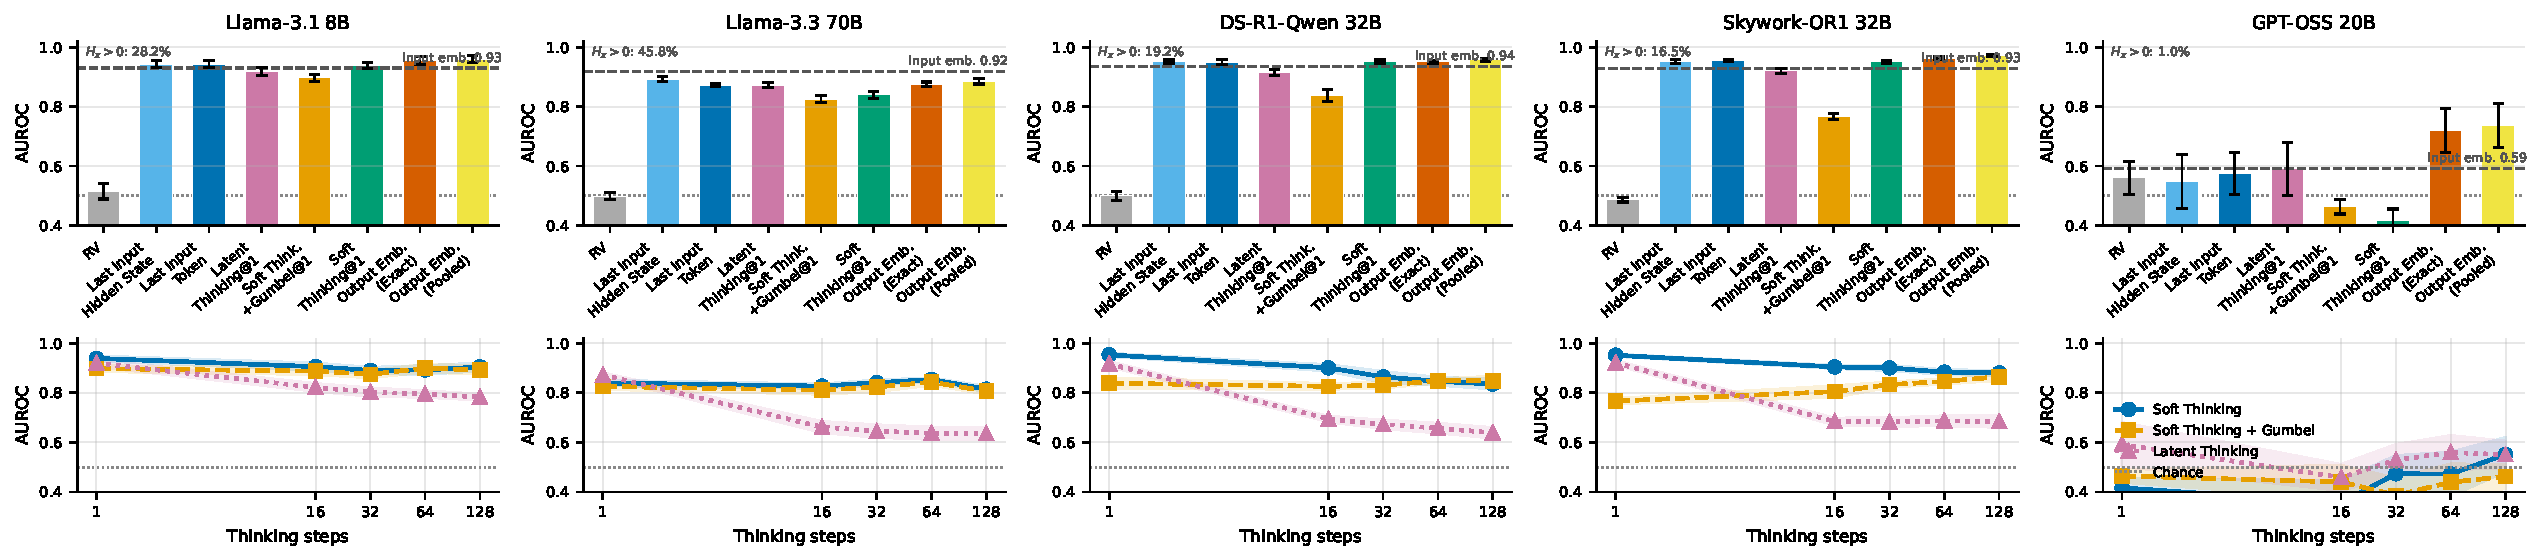
\includegraphics[width=0.98\linewidth]{figures/pdf/dcs_stability.pdf}
  \caption{Distributional Consistency Score (DCS) across source LLMs at $\tau=0.9$.
    Top row, AUROC of the difference-of-means probe predicting $H_x > 0$ from each thought representation, with the input embedding shown as a question-difficulty baseline.
    Bottom row, DCS as a function of thinking steps for the iterative thought families.}
  \label{fig:dcs-stability}
\end{figure}


The Minimality residual $\Delta_{\text{IB}}$ in
\cref{tab:minimality-delta-ib} is read within source LLM. The absolute
sign and scale of $\Delta_{\text{IB}}$ shift across source LLMs because
the cross-entropy decomposition discards a TR-independent constant
whose value depends on the conditional entropies of $X$ and $Y$ for
that LLM, and recovering the absolute IB Lagrangian requires this
constant (\cref{appendix:sub:minimality_ib_derivation}).
The within-LLM ranking of candidates is the meaningful comparison.
\Cref{fig:results_summary} in the main text applies this within-LLM
normalisation directly so that all four axioms appear on a comparable
within-LLM scale.

\subsection{Distributional Views of Causality}
\label{appendix:sub:distributional_views}

\cref{tab:causality-results} reduces each candidate to a single number per source LLM.
We complement that view with two diagnostics that read the same per-problem records bootstrapped in \cref{appendix:sub:bootstrap}, without reweighting or new measurements.

\cref{fig:causality-kl-pooled-cdf} pools all per-beam KLs at the $50$-token
window into one distribution per representation and reports its CDF, with
one panel per representation family. A curve sitting to the left has smaller
per-problem KL on average. A steeper curve has a tighter per-problem
distribution around the mean reported in \cref{tab:causality-results}. A
curve that approaches the top slowly has a heavy upper tail of high-KL
problems that pulls the mean above the per-problem median. With this
reading, the anchor panel separates candidates that the mean alone
clusters into a single rank, since Exact output embedding lands at a similar
mean as Random vector but carries a longer upper tail. Within the thinking
families, increasing the step count shifts the entire distribution rather
than only its mean, and Soft thinking with Gumbel noise at $32$ steps shows
a particularly heavy upper tail that is invisible at the mean.

\cref{fig:causality-kl-variance} decomposes the KL dispersion into
between-problem and within-problem components. Values close to $1$ indicate
that the per-problem mean is carried by problem-level differences, supporting
the cluster-bootstrap design of \cref{appendix:sub:bootstrap}, while values close
to $0$ indicate that the dispersion lives across beams within a single
problem, so the mean averages over a heterogeneous within-problem
distribution.
The Random Vector and Output Embedding anchors show low ICC values, indicating that their per-beam KL dispersion is concentrated within individual problems rather than driven by problem-level differences.
The soft-thinking and latent-thinking families show high ICC, so the scalar mean reported in \cref{tab:causality-results} is a stable per-problem property rather than an average over heterogeneous within-problem noise.

\begin{figure}[t]
  \centering
  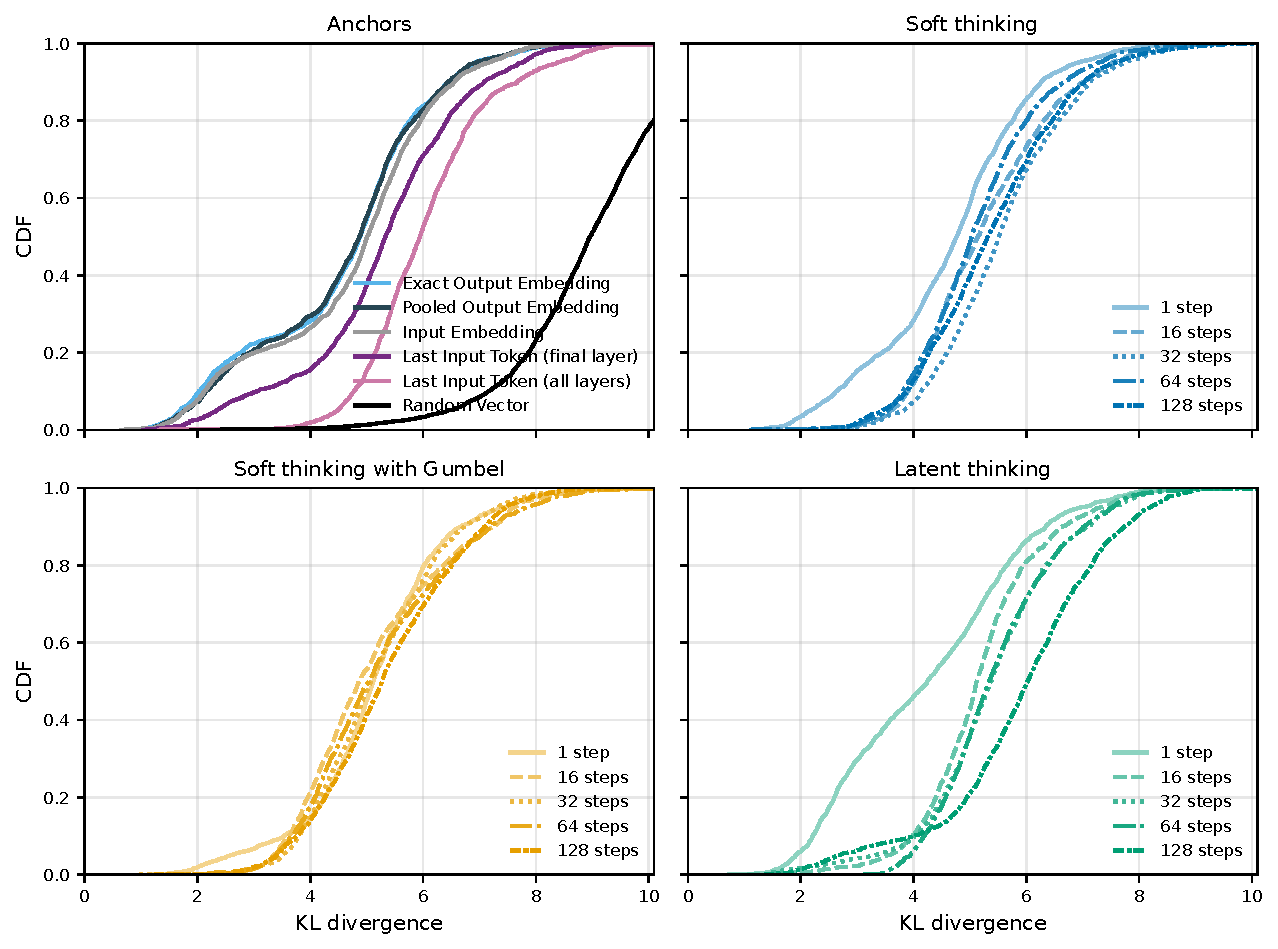
\includegraphics[width=\linewidth]{figures/pdf/causality_kl_pooled_cdf_70b.pdf}
  \caption{Per-beam KL CDFs at the $50$-token averaging window on Llama-3.3-70B, with one panel per representation family (anchor candidates, soft thinking, soft thinking with Gumbel noise, latent thinking). Within each thinking family every step count is shown.}
  \label{fig:causality-kl-pooled-cdf}
\end{figure}

\begin{figure}[t]
  \centering
  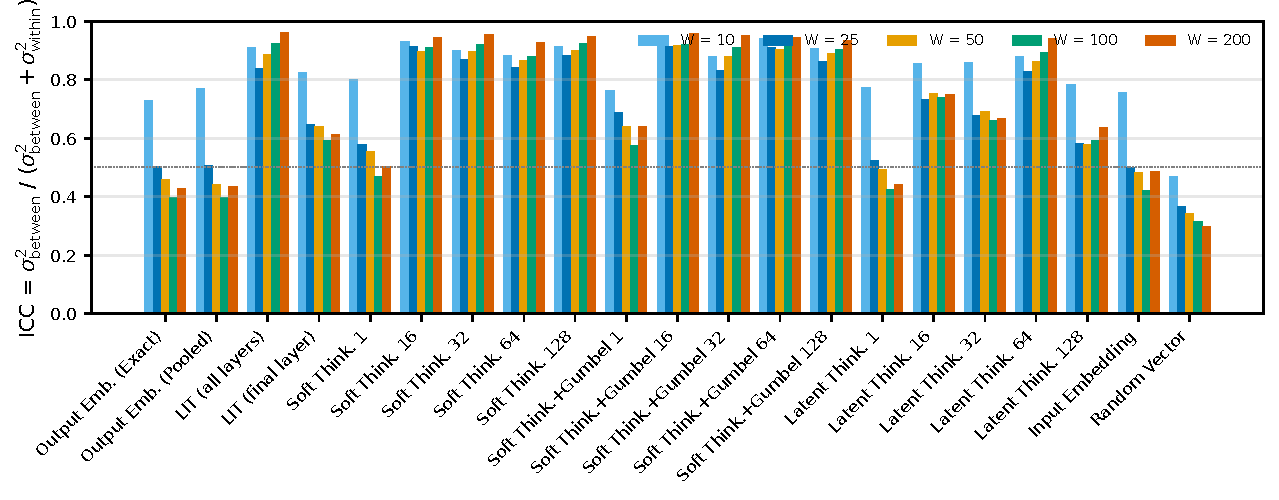
\includegraphics[width=\linewidth]{figures/pdf/causality_kl_variance_70b.pdf}
  \caption{Intraclass correlation $\mathrm{ICC} = \sigma^2_{\text{between}} / (\sigma^2_{\text{between}} + \sigma^2_{\text{within}})$ of per-beam causality KL on Llama-3.3-70B, with bars per averaging window. Values above $0.5$ indicate that the per-problem mean carries most of the dispersion, validating the cluster bootstrap that resamples problems and keeps within-problem beams glued together (\cref{appendix:sub:bootstrap}).}
  \label{fig:causality-kl-variance}
\end{figure}


\subsection{Causality with the Output-Reconstruction Projection}
\label{appendix:sub:causality_minproj}


The headline Causality results in \cref{tab:causality-results} use the projection trained under the language-modelling objective of the Minimality output probe. The Minimality probe learns a projection of the same shape as the discriminator's, mapping $\mathbf{T}$ into the embedding space of the frozen $1$B model, but optimised to reconstruct $Y$ rather than to solve a binary discrimination task. We document here the ablation that motivated this choice.

We test whether the projection objective is the bottleneck for Causality by substituting the discriminator-trained projection in place of the output-reconstruction projection. Each representation is evaluated at its native substitution length without tiling, so the comparison isolates the projection objective from the length effects examined in \cref{appendix:causality_length}. The substitution path and KL formula are otherwise unchanged, and the random-vector reference column controls for any fixed projection-induced shift.

\cref{tab:causality-minproj-70b} reports the comparison on Llama-3.3-70B for the four representations of \cref{methodology}. The output-reconstruction projection meaningfully lowers KL for the latent representations that already live on the source-model manifold, with soft thinking dropping by roughly half on the KL scale and last input token by a smaller but separable margin. The exact output embedding moves the other way and the random-vector reference is unchanged, confirming the effect is representation-specific rather than a fixed projection-induced shift. The discriminator-projection numbers are retained in \cref{tab:causality-disc} for cell-by-cell comparison.

% Causality projection-swap ablation on Llama-3.3-70B.
% Source: outputs/ablations/causality/llama_70b_minproj.csv (n=409 paired problems).

\begin{table}[!htbp]
  \centering
  \footnotesize
  \setlength{\tabcolsep}{6pt}
  \renewcommand{\arraystretch}{1.15}
  \begin{tabular}{@{}l c c c@{}}
    \toprule
    Representation & $\mathrm{KL}_{\mathrm{Disc}}$ & $\mathrm{KL}_{\mathrm{LM}}$ & Paired $\Delta$ (95\% CI) \\
    \midrule
    Exact output embedding         & $4.90$ & $5.33$ & $+0.43\ [+0.28, +0.57]$ \\
    Last input token (all layers)  & $7.41$ & $5.99$ & $-1.42\ [-1.55, -1.30]$ \\
    Soft thinking, $128$ steps     & $10.51$ & $5.49$ & $-5.02\ [-5.22, -4.82]$ \\
    Random vector                  & $4.44$ & $4.39$ & $-0.05\ [-0.10, +0.01]$ \\
    \bottomrule
  \end{tabular}
\caption{Causality KL ($\downarrow$) on Llama-3.3-70B comparing the discriminator-trained projection (\cref{tab:causality-disc}; Disc) against the output-reconstruction projection used in the main text (\cref{tab:causality-results}; LM). The paired column reports the per-problem mean of $\mathrm{KL}_{\mathrm{LM}} - \mathrm{KL}_{\mathrm{Disc}}$ with cluster-bootstrap $95\%$ CI; entries with the entire CI on one side of zero are statistically separable from the projection used in the main text.}
\label{tab:causality-minproj-70b}
\end{table}


The projection objective is accordingly a substantial contributor to the high KL values in \cref{tab:causality-results} for representations native to the source-LLM residual stream, where switching to the output-reconstruction projection yields representation-specific reductions while the random-vector reference remains unchanged.

\subsection{Information-Bottleneck Decomposition for the Minimality Metric}
\label{appendix:sub:minimality_ib_derivation}

The minimality metric $\Delta_{\text{IB}}$ of \cref{methodology} is the Information Bottleneck Lagrangian at the symmetric weight $\beta = 2$, expressed in cross-entropies a probe can compute. We give the derivation, identify the constant offset between $\Delta_{\text{IB}}$ and the absolute Lagrangian, and characterise the conditions under which the surrogate is exact.

\paragraph{Chain-rule decomposition.} The general chain rule for mutual information reads $I(X; \mathbf{T}) + I(Y; \mathbf{T} \mid X) = I(\mathbf{T}; Y) + I(X; \mathbf{T} \mid Y)$. When $\mathbf{T}$ is a deterministic function of $X$, the term $I(Y; \mathbf{T} \mid X)$ vanishes because $\mathbf{T}$ has no residual variance once $X$ is known, so the chain rule collapses to $I(X; \mathbf{T}) = I(\mathbf{T}; Y) + I(X; \mathbf{T} \mid Y)$. Substituting into the IB Lagrangian $L(\beta) = I(X; \mathbf{T}) - \beta\, I(\mathbf{T}; Y)$ gives $L(\beta) = (1 - \beta)\, I(\mathbf{T}; Y) + I(X; \mathbf{T} \mid Y)$. At $\beta = 2$ the two coefficients have equal magnitude with opposite signs, recovering the symmetric trade-off
\begin{equation}\label{eq:ib-decomposition}
    -L(2) = I(\mathbf{T}; Y) - I(X; \mathbf{T} \mid Y)
\end{equation}

\paragraph{Barber--Agakov surrogates.} Mutual information is intractable because $H(\cdot \mid \cdot)$ depends on unknown distributions. For any approximate conditional $q$, Gibbs' inequality gives $H(A \mid B) \le \text{CE}_q(A \mid B)$, with equality iff $q$ matches the true conditional. Training a probe to minimise empirical negative log-likelihood on $(B, A)$ pairs therefore yields a tight upper bound on $H(A \mid B)$ in the limit of a sufficiently expressive probe class. We use this to estimate the two terms of $-L(2)$,
\begin{align}
    I(\mathbf{T}; Y) &= H(Y) - H(Y \mid \mathbf{T}) \;\approx\; H(Y) - \text{CE}(Y \mid \mathbf{T}), \label{eq:ib-surrogate-y} \\
    I(X; \mathbf{T} \mid Y) &= H(X \mid Y) - H(X \mid Y, \mathbf{T}) \;\approx\; \text{CE}(X \mid Y) - \text{CE}(X \mid Y, \mathbf{T}). \label{eq:ib-surrogate-x}
\end{align}
The first follows from the standard Barber--Agakov lower bound on mutual information~\citep{barber2003variational}. The second is its conditional analogue, where two probes share the input $Y$ and differ only in whether $\mathbf{T}$ is appended.

\paragraph{Reduction to \texorpdfstring{$\Delta_{\text{IB}}$}{IB}.} Substituting the surrogates into $-L(2)$ and grouping $\mathbf{T}$-dependent terms,
\begin{equation}\label{eq:ib-reduction}
    -L(2) \;\approx\; \big[\text{CE}(X \mid Y, \mathbf{T}) - \text{CE}(Y \mid \mathbf{T})\big] + \big[H(Y) - \text{CE}(X \mid Y)\big] = \Delta_{\text{IB}} + C
\end{equation}
The constant $C = H(Y) - \text{CE}(X \mid Y)$ depends only on the dataset and the unconditional baseline probe, not on the candidate $\mathbf{T}$. Comparisons of $\Delta_{\text{IB}}$ across representations are therefore comparisons of $-L(2)$ shifted by a single offset.

\paragraph{Bounding direction and ranking preservation.} By Gibbs' inequality each CE term upper-bounds the corresponding conditional entropy, so each approximation in \cref{eq:ib-surrogate-y,eq:ib-surrogate-x} yields a lower bound on the mutual information term it estimates. In $\Delta_{\text{IB}}$, however, the two CE approximations are subtracted from each other. Any systematic bias shared across candidates that is absorbed into the constant $C$ cancels in the difference. Within a fixed probe class and a fixed source LLM, the residual approximation error is candidate-independent, so the ranking of $\Delta_{\text{IB}}$ across thought representations is preserved. This is why the metric is read within a source LLM rather than across LLMs, as $C$ varies with the source LLM's output distribution and must not be compared across models.

\paragraph{Random Vector cross-entropy interpretation.} The elevated $\text{CE}(Y \mid \mathbf{T})$ observed for the Random Vector anchor is not an out-of-distribution artifact. A random vector carries no information about $Y$, so a probe conditioned on pure noise cannot predict the output sequence and cross-entropy rises to the level of an unconditional language model. The probe is asked to optimize a signal that does not exist in $\mathbf{T}$, and the resulting high CE confirms that the metric correctly identifies the absence of output-relevant content rather than a distributional mismatch.

\paragraph{When the chain-rule assumption fails.} The reduction relies on $I(Y; \mathbf{T} \mid X) = 0$. The exact output embedding and pooled output embedding candidates are computed directly from the generated continuation, so $\mathbf{T}$ is a function of $Y$ as well as $X$ and $I(Y; \mathbf{T} \mid X) > 0$. For these rows, the substitution into the Lagrangian carries a correction term that does not collapse into a TR-independent constant, so $\Delta_{\text{IB}}$ no longer estimates $-L(2)$ even up to $C$. The reported value still has a clear empirical reading. For the exact output embedding, $\mathbf{T}$ contains $Y$ by construction, so $\text{CE}(Y \mid \mathbf{T})$ collapses toward zero and $\text{CE}(X \mid Y, \mathbf{T})$ approaches $\text{CE}(X \mid Y)$. The metric therefore flags this row as a trivially sufficient anchor with no residual leakage, which is the correct behavioural diagnosis even though the IB-Lagrangian interpretation no longer applies.

\subsection{Length Sensitivity of the Causality Metric}
\label{appendix:causality_length}

The causality KL in \cref{tab:causality-results} averages over the last $50$ tokens of each generated beam, which raises two length-based concerns. First, the metric might track prompt size rather than thought content. Second, a longer generation alone could inflate KL for whichever candidate happens to produce it. \cref{fig:causality-length-correlation} examines both.

The first concern is ruled out outright. No candidate shows a meaningful coupling between KL and input length, so the main-text ordering does not reflect task-to-task variation in prompt size.

The second concern resolves cleanly. Output length couples with KL only for the Random Vector lower-bound reference, since its content is uninformative by construction and longer generations accumulate more positions that disagree with the explicit prefix and inflate its KL on long beams. The candidates clearly below this reference in \cref{tab:causality-results} show near-zero coupling, so their KL is driven by representational fit rather than by how much the source model chose to generate. Output length is therefore not a competing explanation for the main-text ranking but a property of the lower-bound reference against which the ranking is measured.

\begin{figure}[t]
  \centering
  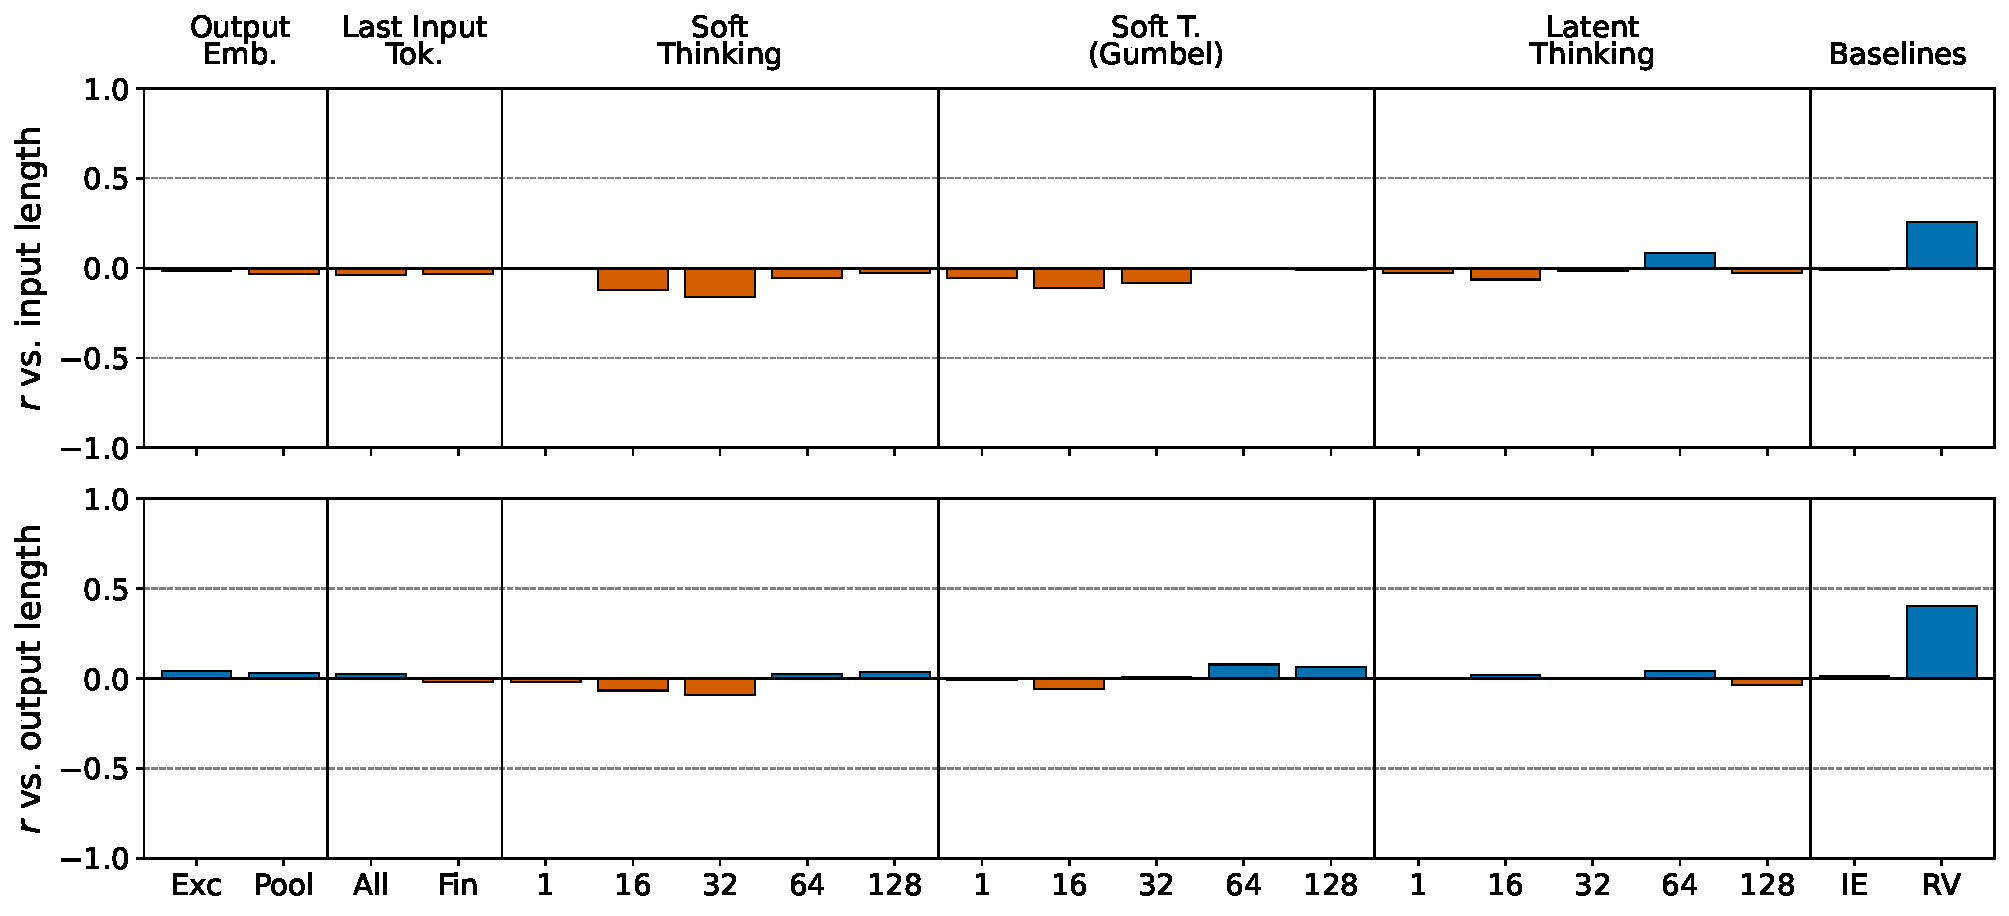
\includegraphics[width=0.95\linewidth]{figures/pdf/causality_length_correlation.pdf}
  \caption{Pearson $r$ between per-example causality KL and input length (top) or output length (bottom), in characters, on Llama-3.1-8B-Instruct. Candidates follow the order of \cref{tab:causality-results}.}
  \label{fig:causality-length-correlation}
\end{figure}


We further test whether the choice of $50$ tokens itself drives the ranking by recomputing the metric across windows of $\{10, 25, 50, 100, 200\}$ tokens at no extra source-LLM cost, since each beam saves a per-window KL during a single causality pass through the discriminator. \cref{fig:causality-window-sweep} shows the result. The coarse ordering between candidates is stable across windows, with strong candidates sitting near the bottom of the KL axis and weak candidates near the top at every scale, so the ranking in \cref{tab:causality-results} does not depend on the exact window length. Fine-grained orderings within clusters of similarly-performing candidates do shift at the longer windows, where the shared $Z$ context narrows absolute differences to the point that small method-to-method gaps become statistically indistinguishable. At the shortest window the metric averages over very few positions, where per-token stochastic variance dominates and no candidate cleanly separates from the floor. The $50$-token window sits between these two extremes, giving the cleanest separation between candidates while still averaging over enough positions to be statistically stable.

\begin{figure}[t]
  \centering
  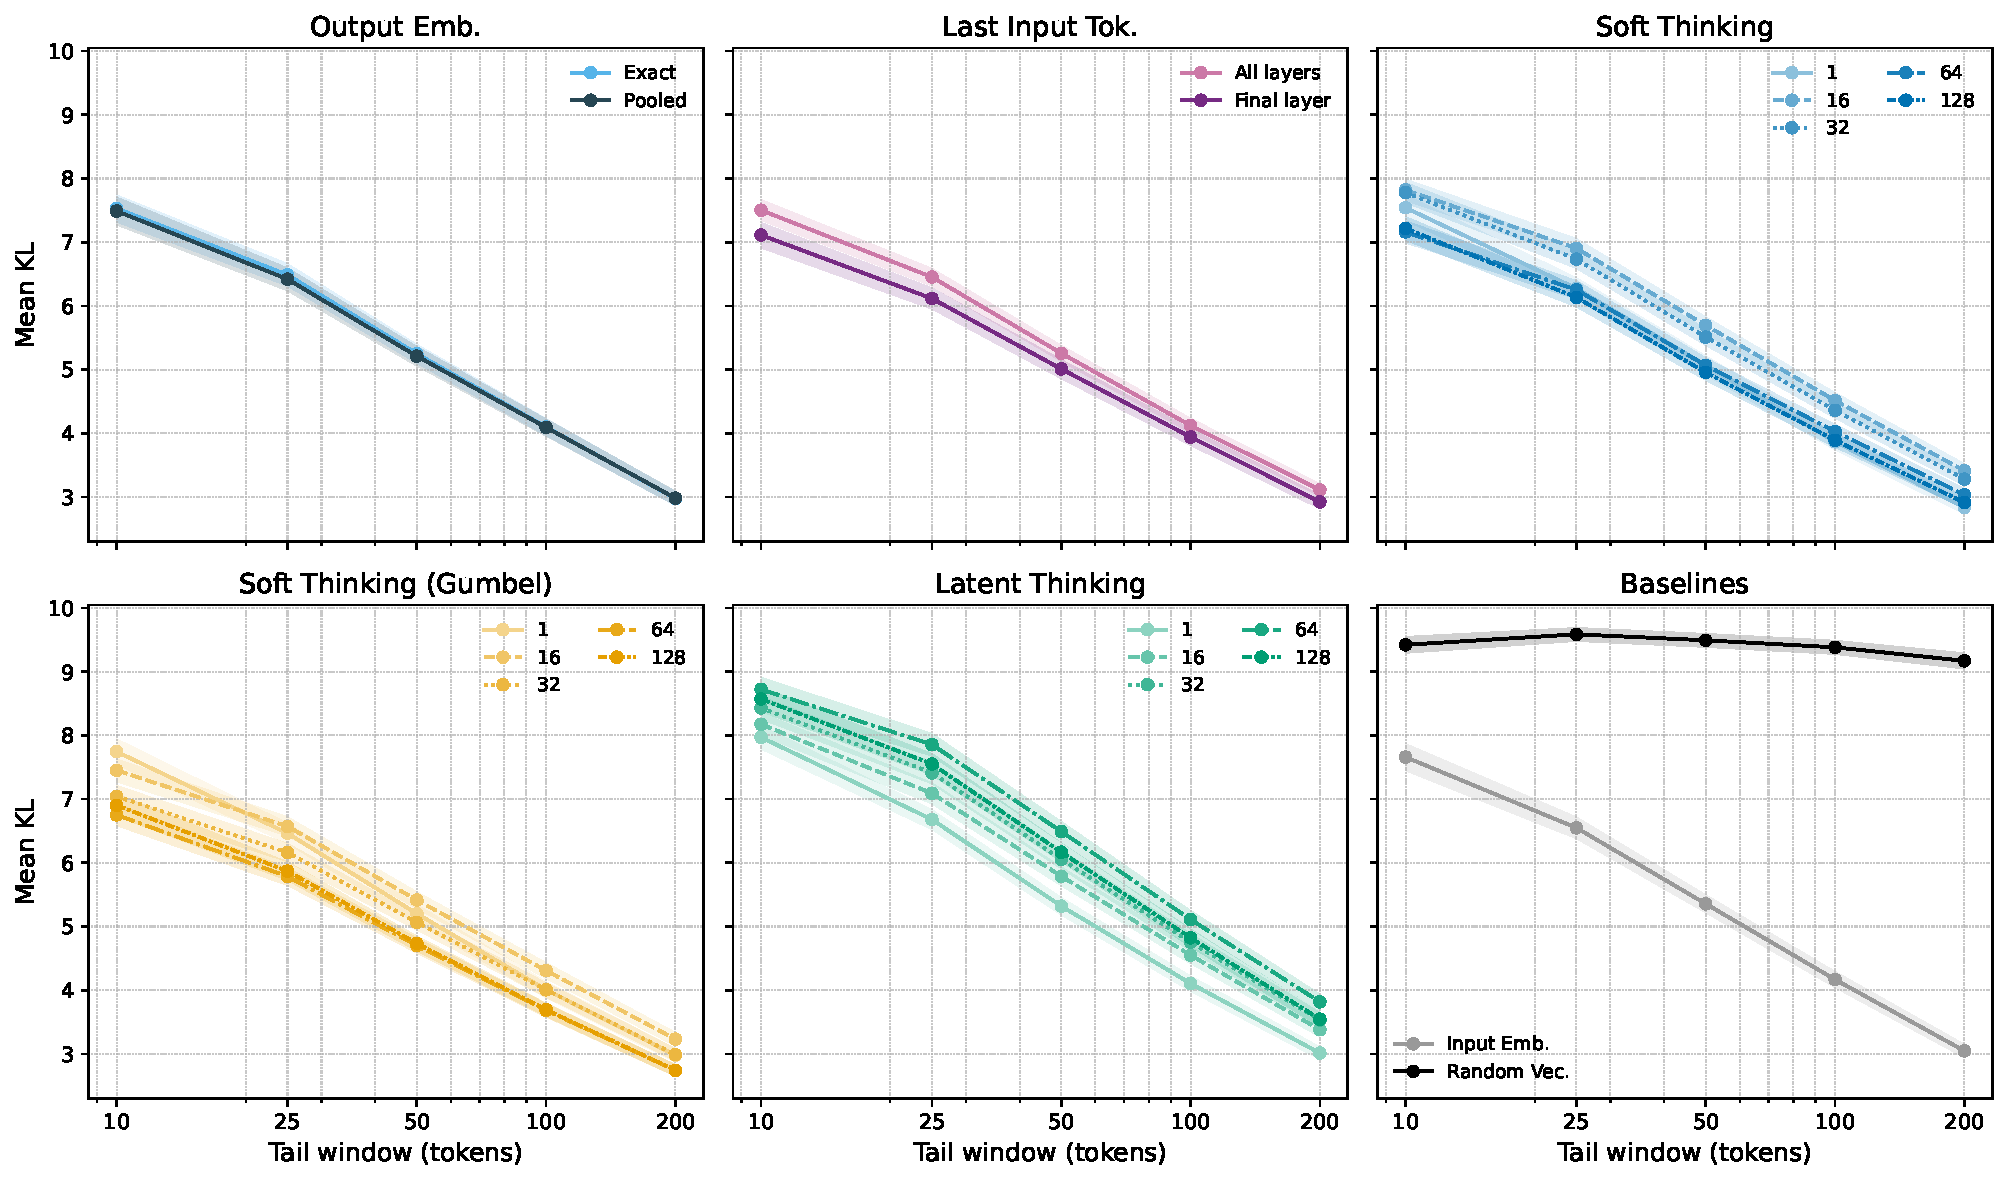
\includegraphics[width=0.95\linewidth]{figures/pdf/causality_window_sweep.pdf}
  \caption{Mean causality KL on Llama-3.1-8B-Instruct across $Z$-windows of $\{10, 25, 50, 100, 200\}$ tokens, with $95\%$ bootstrap CI bands. One panel per TR family, one line per (TR type, think steps) tuple.}
  \label{fig:causality-window-sweep}
\end{figure}


A third length-based concern is the number of substituted vector positions itself, which varies across candidates. Last input token (all layers) substitutes one position per source-model layer, Soft thinking substitutes one position per thinking step, while embedding candidates substitute a single position. To isolate the geometric effect of substitution length from any change in information content, we tile each candidate to a common number of positions and recompute KL. \cref{fig:causality-kl-vs-length} reports the result on Llama-3.3-70B for the four candidates from \cref{tab:causality-results} that admit clean tiling.

The Random vector curve rises markedly with substitution length, even though its content is by construction uninformative about the prefix, and the same trend appears for Exact output embedding with a smaller dynamic range. Substitution length therefore inflates KL on candidates that carry no instance information, which establishes that absolute KL magnitudes are not commensurable across candidates of different native lengths. The relative ordering between candidates also reorganises once length is matched, with candidates that sat at the strong end of the table at native length sliding toward the weak end once they are tiled out to the length of the longer candidates. The reorganisation does not nullify \cref{tab:causality-results}, since tiling a one-position candidate produces a rank-one substitution that is structurally different from a natively multi-position candidate, but it does mean that absolute KL gaps in the table reflect a mix of representational quality and substitution geometry.

This finding fixes the methodological choice that all subsequent quantitative comparisons feed $\mathbf{T}$ at a common substitution length, so that no representation is rewarded or penalised by the metric simply for being natively shorter or longer than another. The causality results of \cref{tab:causality-results} and the minimality probes underlying \cref{tab:minimality-delta-ib} both adopt the same tiled length, and varying-length comparisons are reserved for the diagnostic in \cref{fig:causality-kl-vs-length}.

\begin{figure}[t]
  \centering
  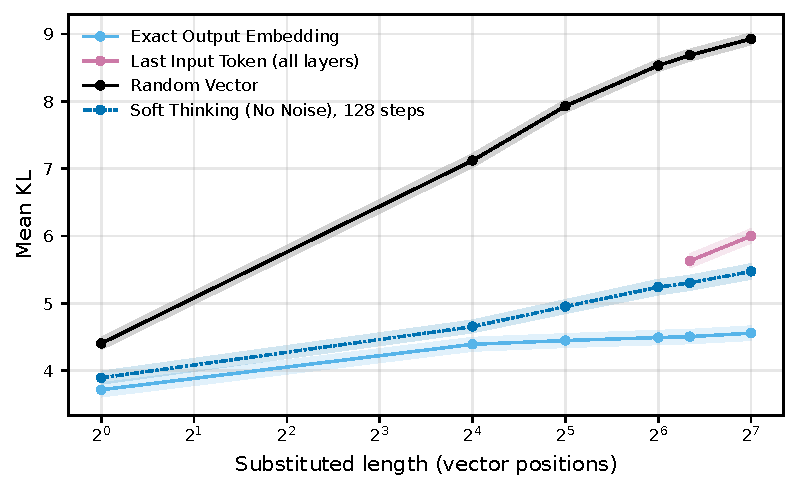
\includegraphics[width=0.78\linewidth]{figures/pdf/causality_kl_vs_length_70b.pdf}
  \caption{Mean causality KL on Llama-3.3-70B as the substituted length $L$ varies, with $95\%$ cluster-bootstrap CI bands. The single-vector candidates (Exact Output Embedding, Random Vector) are repeated $L$ times. Soft Thinking (No Noise) uses its native $128$-step trajectory truncated to its first $L$ vectors at $L\le 128$, so different $L$ points cover different prefixes of the same trajectory rather than tiled copies of one vector. Last Input Token (all layers) has native length $81$ on Llama-3.3-70B and is shown at $L=81$ (no tiling) and at $L=128$ (the stack is wrapped to fill the substitution window).}
  \label{fig:causality-kl-vs-length}
\end{figure}


\subsection{Geometric Analysis of Representational Collapse}
\label{appendix:geometric}

\cref{tab:disc-results} reports near-ceiling cross-task discrimination on most candidates and near-random same-task discrimination on almost all of them, which invites the objection that the same-task failure reflects probe capacity rather than a property of the representation. We address this objection by measuring the thought-vector geometry directly, with no trained probe in the loop. Each candidate is flattened to a single vector per problem (the full $L{\times}d$ hidden-state stack for LIT, the $s{\times}d$ prefix for $s$-step thinking candidates), and all comparisons use cosine similarity.

\paragraph{Two quantities, one per discriminator task.}
\begin{itemize}[leftmargin=1.6em,itemsep=3pt,topsep=2pt]
  \item \textbf{$k$-NN task purity} \citep{wu2018unsupervised, caron2021emerging} at $k{=}10$. For each thought vector, purity is the fraction of its ten nearest neighbours (by cosine similarity) that carry the same task label. The average over all vectors lies in $[0, 1]$, with uniform random neighbour assignment giving $\approx 0.042$, and a value near $1$ means the geometry clusters problems by task.
  \item \textbf{Within-task participation ratio} \citep{litwinkumar2017optimal, recanatesi2019dimensionality} $\mathrm{PR} = \bigl(\sum_i \sigma_i^2\bigr)^2 / \sum_i \sigma_i^4$, where $\sigma_i$ are the singular values of the centred matrix of within-task vectors for a given task (so $\sigma_i^2$ are the eigenvalues of its sample covariance), averaged over tasks. $\mathrm{PR}$ counts how many directions are needed to describe the within-task variance, ranging from $1$ when every within-task vector points the same way up to $N{-}1$ when the vectors spread over as many orthogonal directions as centering allows, where $N$ is the number of within-task problems. On this split $N \approx 20$, so the ceiling is $\approx 19$, and Random Vector reaches $\mathrm{PR} = 18.5$ close to that ceiling.
\end{itemize}

Each clustering quantity tracks one discriminator. Purity must clearly exceed the random-neighbour baseline for cross-task discrimination to succeed, since no probe can recover task structure that is absent from the geometry. $\mathrm{PR}$ must clearly exceed $1$ for same-task discrimination to succeed, since two within-task vectors that span too few directions are too close together for any learned projection to pull apart. The converse is weaker, because Random Vector achieves the maximum $\mathrm{PR}$ by construction and so a high $\mathrm{PR}$ alone cannot certify that the within-task directions encode instance content. Geometry therefore detects the two failure modes (low purity or low $\mathrm{PR}$) without relying on probe behaviour, but cannot certify success.

\paragraph{An anisotropy-adjusted similarity scale.}
We complement the two clustering quantities with a third diagnostic, the within-task self-similarity adjusted for anisotropy, following \citet{ethayarajh2019contextual}. Define $\Delta_{\cos} = \overline{\cos}_{\text{within-task}} - \overline{\cos}_{\text{cross-task}}$, where the cross-task pair mean serves as the anisotropy baseline inherent to self-attention \citep{godey2024anisotropy}. Subtracting this baseline isolates the within-task scale beyond what transformer geometry alone produces. Where \citet{ethayarajh2019contextual} apply the adjustment at the token level, we compute it on flattened example-level vectors so that a single number summarises each candidate. $\Delta_{\cos}$ is orthogonal to $k$-NN purity and $\mathrm{PR}$, since it varies in similarity scale rather than in cluster structure.

\begin{figure}[!htbp]
  \centering
  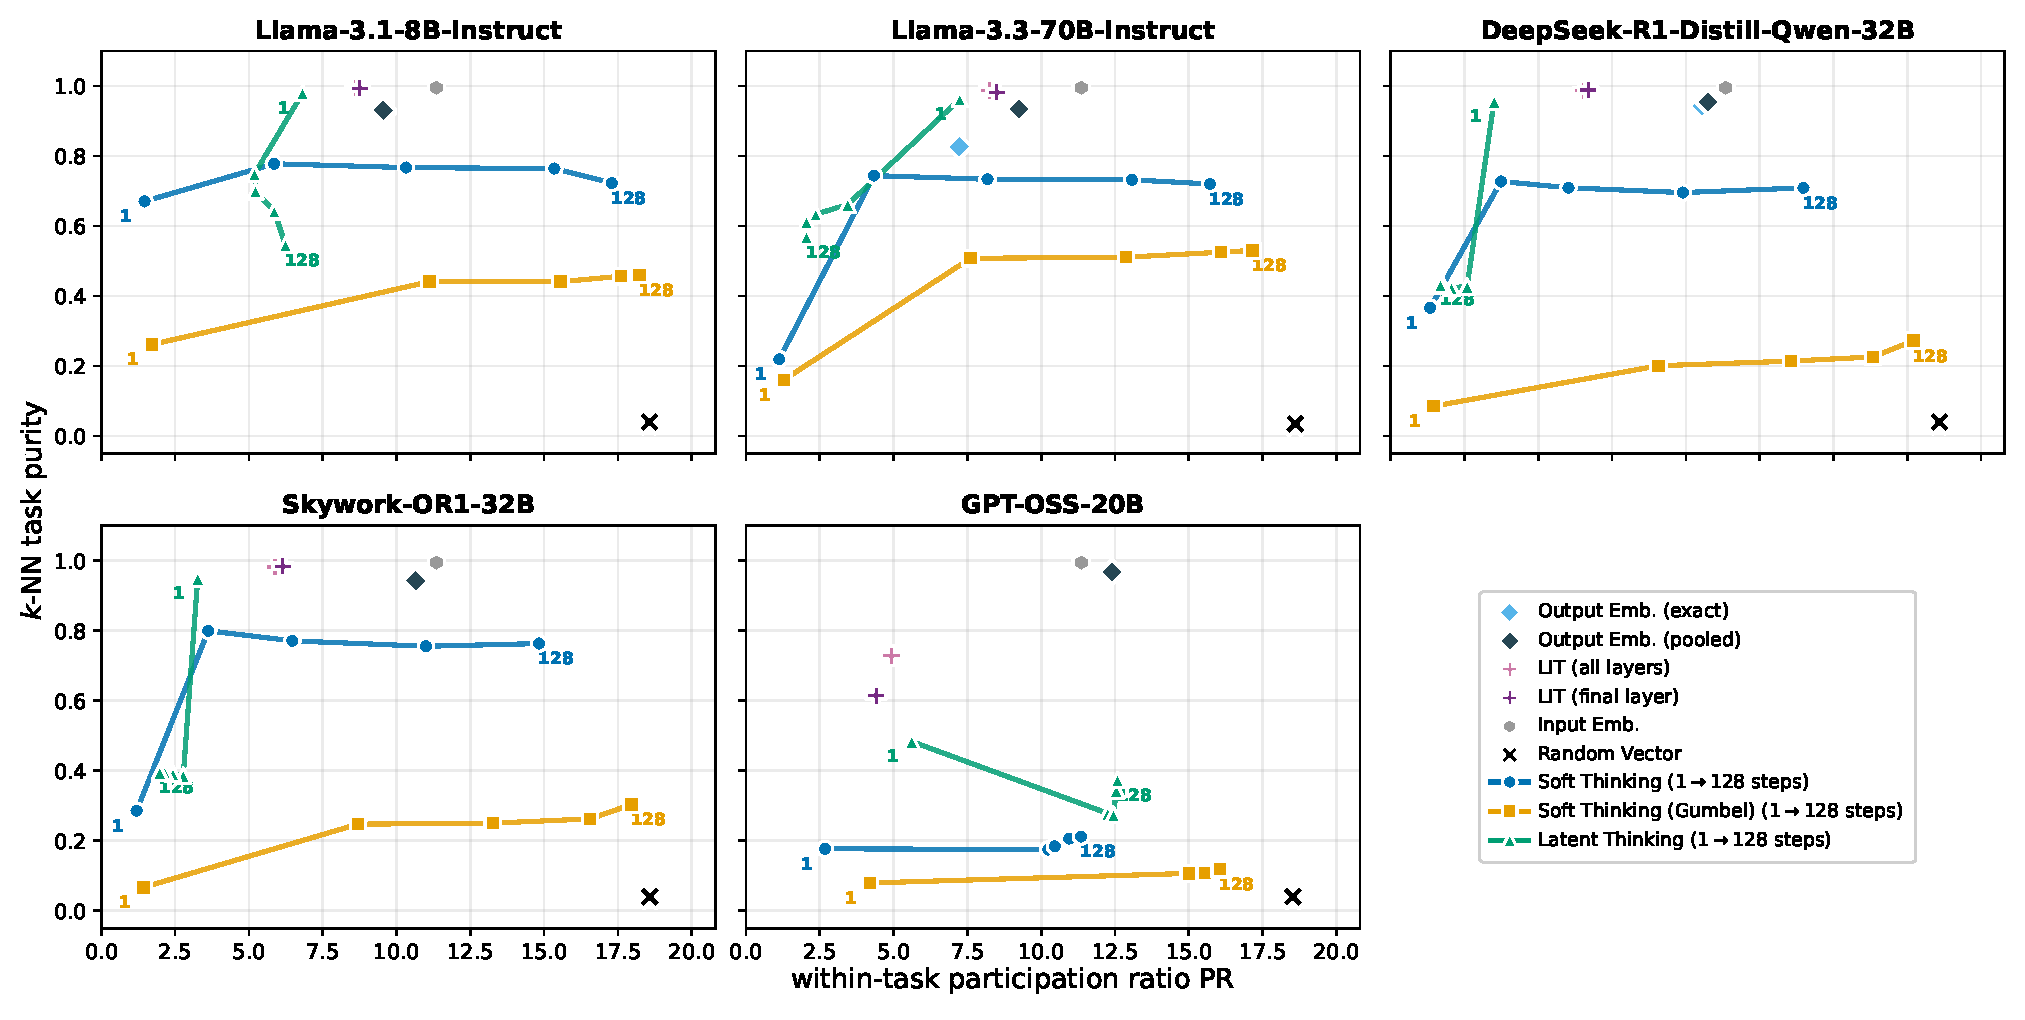
\includegraphics[width=0.98\linewidth]{figures/pdf/geom_summary_multi.pdf}
  \caption{Each candidate placed on the $(\mathrm{PR}, k\text{-NN purity})$ plane, one panel per LLM. Solid lines trace thinking-family trajectories as the step count grows from $1$ to $128$. Candidates further to the upper right are preferable: higher $\mathrm{PR}$ indicates a within-task subspace spread across more directions, and higher $k$-NN purity indicates that nearest neighbours are drawn from the same task.}
  \label{fig:geom-summary}
\end{figure}


\cref{fig:geom-summary} places every candidate on the $(\mathrm{PR}, \text{purity})$ plane for each LLM, and the top-right region remains empty in every panel. LIT, Latent Thinking at one step, Input Embedding, and the two Output Embedding candidates occupy the same region of the plane on four of the five LLMs, with moderate $\mathrm{PR}$ below the ceiling and high purity; on GPT-OSS-20B both LIT variants drop to lower purity while the Output and Input Embedding candidates stay in their usual region. The geometry therefore admits cross-task discrimination but constrains within-task variance to a narrow subspace regardless of architecture or size. Output Embedding candidates land in this same cluster yet still succeed at same-task discrimination in \cref{tab:disc-results}, because their within-task directions encode instance content that LIT's do not. Geometry alone cannot tell the two cases apart, so the analysis rules out failure without certifying success.

Same-task discrimination fails because the within-task geometry of latent thought representations is itself collapsed, either too narrow (low $\mathrm{PR}$), too noise-drifted (low purity), or both, and this holds across every LLM tested. Probe capacity therefore cannot explain the failure. Latent Thinking begins at one step in the high-purity region near LIT on every LLM, but adding latent steps cuts purity by roughly half on each LLM and additionally sheds $\mathrm{PR}$ on the larger Llama and on both distilled and RL-trained reasoning models. Soft Thinking begins in the opposite low-$\mathrm{PR}$ corner and gains $\mathrm{PR}$ steadily as depth grows, but $\Delta_{\cos}$ contracts in step with the gain (from $\sim 0.30$ at one step to $\sim 0.09$ at $128$ on the Llama models), so the additional dimensions opened up by depth carry less, not more, anisotropy-adjusted within-task signal. Soft Thinking with Gumbel noise traces the same rightward path at consistently lower purity and lands at $\Delta_{\cos} \in [0.02, 0.05]$ across all five LLMs, indistinguishable from Random Vector on that axis. No trajectory in any panel enters the high-$\mathrm{PR}$, high-purity, high-$\Delta_{\cos}$ region occupied by LIT and Output Embedding. The verdict is uniform across architectures and sizes. The distilled and RL-trained reasoning models produce nearly identical panels in \cref{fig:geom-summary}, with every clustering quantity and similarity scale agreeing to within a few percent across all candidates and only minor offsets in the Latent and Soft Thinking trajectories.

The geometric verdict matches the main-text tables across LLMs. Every candidate apart from Output Embedding has either low $\mathrm{PR}$ or low purity in each panel, and all of them fail same-task discrimination in \cref{tab:disc-results}. The $\mathrm{DCS}$ floor in \cref{tab:dcs} shares the same origin, because cosine similarity over a narrow or noise-drifted within-task subspace cannot reproduce a richer semantic equivalence matrix at any threshold. The picture is therefore consistent across architectures and sizes. The failure to discriminate within a task is a property of the geometry that latent computation produces, not an artifact of any single LLM.

$\Delta_{\cos}$ anchors the same picture on the scale axis. Random Vector is at the lower bound near $0$, Input Embedding at the upper bound near $0.52$, and LIT and Output Embedding occupy a range between roughly $0.18$ and $0.45$. All three diagnostics converge on the same failure pattern, and none depend on a trained discriminator.

\subsection{Probe Capacity Ablation}
\label{appendix:capacity_ablation}

\Cref{appendix:geometric} ruled out the most direct version of the weak-probe objection at the level of the geometry itself, with no trained classifier in the loop. We add a complementary line of defense within the probe-based metric by varying the same-task discriminator's capacity on the largest source model, Llama-3.3-70B, and showing that the chance-level same-task verdict for the latent-thinking and last-input-token candidates is invariant under three architectures of strictly increasing capacity.

The Baseline architecture, used throughout the main paper, projects the source hidden state into the input space of the frozen $1$B model through a single linear layer. The Deep projection replaces the linear with a two-layer MLP and a LayerNorm. The Deep projection $+$ UF2 architecture additionally unfreezes the last two transformer blocks of the $1$B model. Each step strictly enlarges the trainable-parameter budget, and the deepest tier carries roughly an order of magnitude more trainable parameters than the Baseline.

Three thought representations are evaluated as anchors. Last Input Token and Soft Thinking at $128$ steps are the focus of the same-task failure mode in the main results. Output Embedding (Exact) acts as the positive control, since it is computed from the generated answer itself. If any architecture has a chance to descend below the random-guess plateau, it should descend on this representation.

% Probe capacity ablation on Llama-3.3-70B same-task discrimination.
% Three architectures of strictly increasing capacity vs. three thought
% representations chosen as anchors. Cells report (test accuracy,
% tail-50 mean training BCE). $\ln 2 \approx 0.693$ marks random guess.
% Numbers are pulled directly from the corresponding training logs in
% ~/hidden/logs/disc_70b_parallel/ (Baseline) and
% ~/hidden/logs/disc_70b_deep_ablation/ (Deep / Deep+UF2).

\begin{table}[!htbp]
  \centering
  \footnotesize
  \setlength{\tabcolsep}{6pt}
  \renewcommand{\arraystretch}{1.15}
  \begin{tabular}{@{}l cc cc cc@{}}
    \toprule
                              & \multicolumn{2}{c}{\textit{Baseline}} & \multicolumn{2}{c}{\textit{Deep}} & \multicolumn{2}{c}{\textit{Deep $+$ UF2}} \\
                              & \multicolumn{2}{c}{($\sim 19$M trainable)} & \multicolumn{2}{c}{($\sim 44$M trainable)} & \multicolumn{2}{c}{($\sim 165$M trainable)} \\
    \cmidrule(lr){2-3}\cmidrule(lr){4-5}\cmidrule(lr){6-7}
    Thought representation        & Acc & BCE & Acc & BCE & Acc & BCE \\
    \midrule
    Last Input Token              & $0.516$ & $0.685$ & $0.500$ & $0.693$ & $0.501$ & $0.696$ \\
    Soft Thinking at $128$ steps  & $0.513$ & $0.689$ & $0.511$ & $0.689$ & $0.508$ & $0.692$ \\
    Output Embedding (Exact)      & $0.726$ & $0.494$ & $0.617$ & $0.631$ & $0.642$ & $0.659$ \\
    \bottomrule
  \end{tabular}
\caption{Probe capacity ablation on Llama-3.3-70B same-task discrimination. Each cell reports test accuracy and the tail-$50$ mean of the training BCE loss. Columns increase discriminator capacity from a single linear projection (Baseline) through a deep MLP projection (Deep) to additionally unfreezing the last two transformer blocks of the frozen $1$B backbone (Deep $+$ UF2). $\ln 2 \approx 0.693$ is the BCE value at uniform $0.5$ output and equates to random guess.}
\label{tab:disc-capacity-ablation-70b}
\end{table}


\Cref{tab:disc-capacity-ablation-70b} reports test accuracy alongside the tail-$50$ mean of the training-loss curve, where $\ln 2 \approx 0.693$ is the BCE value at uniform $0.5$ output and equates to random-guess accuracy. Output Embedding (Exact) achieves its highest test accuracy at the Baseline tier ($0.726$), and adding capacity causes overfitting, with test accuracy declining to $0.617$ at the Deep tier and $0.642$ at Deep$+$UF2 despite an order-of-magnitude increase in trainable parameters, while BCE worsens toward the random-guess plateau. Last Input Token and Soft Thinking remain at random-guess accuracy at every capacity tier, with no improvement in accuracy or BCE regardless of how many parameters are available. The Baseline architecture was fixed in pilot experiments and applied consistently across all source LLMs and thought representations (see \cref{appendix:sub:disc_arch}). These ablations confirm post-hoc that it avoids the overfitting induced by deeper tiers while retaining the discriminative accuracy of the positive control. Under the larger architectures, the training loss of the candidates carrying no instance-discriminating content decreases transiently during training, but the tail-$50$ average over held-out steps remains at the plateau, indicating the optimiser learns batch-specific patterns rather than a generalisable structure.

Two independent attacks on the same objection, the geometric one with no probe in the loop and the probe-based one with a probe of increasing capacity, converge on the conclusion that the same-task failure is a property of the representation and not of the discriminator.

\subsection{Relationship to Downstream Task Accuracy}
\label{appendix:downstream}

A natural concern is that within-task separability collapses on hard tasks because the model's output distribution itself becomes less structured under difficulty, not because the representation is inadequate. If this were true, the collapse would track downstream task accuracy and tasks with lower pass@1 would show lower within-task discriminability across all candidates.

\Cref{fig:downstream-correlation} tests this directly by plotting per-task within-task discriminator accuracy against BBEH pass@1 across the 23 BBEH tasks and five LLMs. For thought-representation candidates averaged over the Last Input Token, soft-thinking, latent-thinking, and last-hidden-state families, the pooled Spearman correlation with downstream accuracy is $\rho = 0.10$ ($p = 0.31$, $n = 115$), and no individual LLM reaches significance. The Exact Output Embedding anchor, which has direct access to the generated continuation, also shows no significant correlation ($\rho = 0.14$, $p = 0.13$). Both series are consistent with near-zero correlation across the full range of task difficulties.

These results support the interpretation in \cref{sec:results:per-axiom}. The within-task separability collapse is a property of the thought representations rather than a consequence of tasks being difficult. The framework surfaces representational failures that downstream accuracy does not register.

\begin{figure}[t]
  \centering
  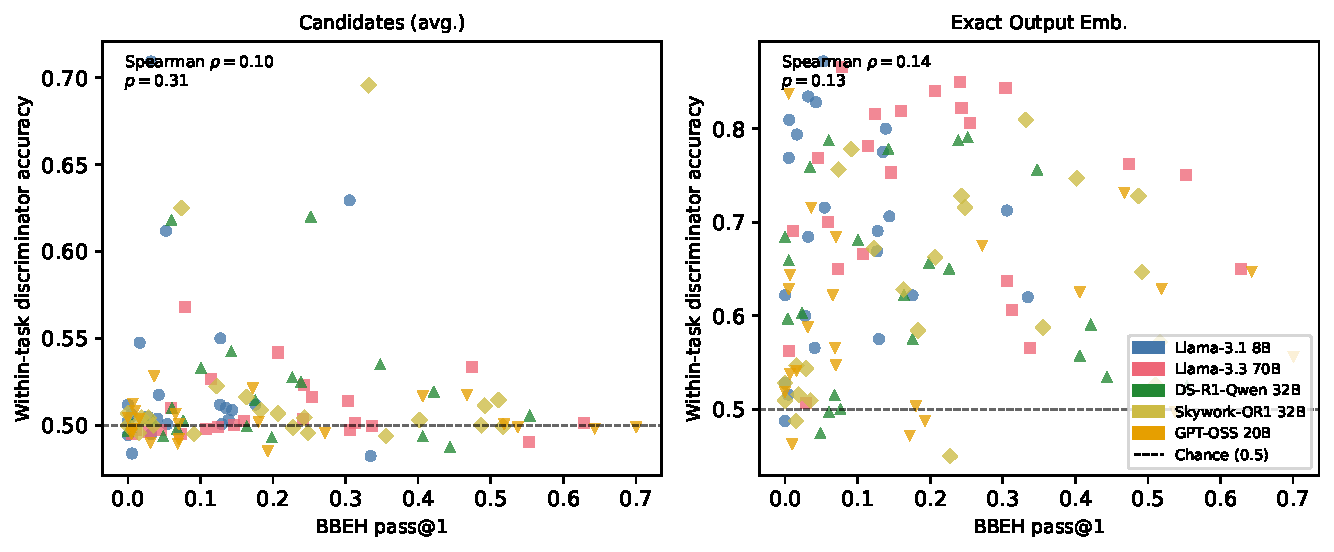
\includegraphics[width=\linewidth]{figures/pdf/downstream_correlation.pdf}
  \caption{Within-task discriminator accuracy versus BBEH pass@1 for candidates
    averaged across Last Input Token, soft-thinking, latent-thinking, and
    last-hidden-state variants (left) and the Exact Output Embedding anchor
    (right), across 23 BBEH tasks and five LLMs. The dashed line marks
    the chance baseline. Spearman $\rho$ and $p$-values are annotated on each
    panel.}
  \label{fig:downstream-correlation}
\end{figure}


\section{Dataset and Benchmark Details}
\label{appendix:dataset}

\subsection{BBEH Task Coverage}
We evaluate on all 23 tasks from BBEH~\citep{kazemi2025bigbenchextrahard}.
Table~\ref{tab:bbeh_tasks} lists the tasks and their categories.
For each task, we use all available examples from the BBEH dataset,
yielding 4{,}520 unique problems across all 23 tasks.
Each problem is expanded to $K=8$ beams during generation, for 36{,}160 beam--problem
pairs in total.
These 4{,}520 problems are further partitioned for probe and discriminator training,
stratified per task: within each BBEH task, problems are randomly shuffled and split
into train / validation / test at an $0.8 / 0.1 / 0.1$ ratio, so every task
contributes proportionally to every split (3{,}616 / 452 / 452 problems in aggregate).

\begin{table}[!htbp]
\vskip 0.15in
\begin{center}
\begin{small}
\begin{sc}
\begin{tabular}{ll}
\toprule
\textbf{Task} & \textbf{Category} \\
\midrule
Boolean Expressions    & Symbolic Reasoning \\
Dyck Languages         & Symbolic Reasoning \\
Multistep Arithmetic   & Quantitative Reasoning \\
Object Counting        & Quantitative Reasoning \\
Time Arithmetic        & Quantitative Reasoning \\
Spatial Reasoning      & Spatial Reasoning \\
Geometric Shapes       & Spatial Reasoning \\
Word Sorting           & Language \\
Hyperbaton             & Language \\
Disambiguation QA      & Language \\
Linguini               & Language \\
Temporal Sequence      & Temporal Reasoning \\
Causal Understanding   & Causal Reasoning \\
Web of Lies            & Social Reasoning \\
Shuffled Objects       & Logical Reasoning \\
Zebra Puzzles          & Logical Reasoning \\
BoardGame QA           & Game Reasoning \\
Buggy Tables           & Tabular Reasoning \\
Movie Recommendation   & Recommendation \\
SportQA                & Factual QA \\
Object Properties      & Commonsense \\
NYC Coordinates (NYCC) & Geography \\
SARC Triples           & Sarcasm Detection \\
\bottomrule
\end{tabular}
\end{sc}
\end{small}
\end{center}
\vskip -0.1in
\caption{BBEH tasks used in our evaluation.}
\label{tab:bbeh_tasks}
\end{table}

Several BBEH tasks build on earlier benchmarks, and we acknowledge the
originating work as requested by the BBEH authors.
BoardGame QA originates from~\citet{kazemi2024boardgameqa}.
Causal Understanding draws on~\citet{nie2024moca} and~\citet{kiciman2023causal}.
Dyck Languages and Word Sorting follow the setup
of~\citet{tyen2023llms}.
Geometric Shapes is based on~\citet{kazemi2023geomverse},
Linguini on~\citet{sanchez2024linguini},
and NYCC builds on~\citet{hessel2022androids}
and~\citet{zhang2024humor}.
Spatial Reasoning follows~\citet{yamada2023evaluating},
Time Arithmetic follows~\citet{fatemi2024test},
Web of Lies follows~\citet{white2024livebench},
and Zebra Puzzles follows~\citet{shah2024causal}.

\subsection{BBEH Answer Extraction}
We use the official BBEH answer extraction logic from
\citet{kazemi2025bigbenchextrahard}, which implements task-specific
regular expression patterns to extract final answers from free-form
model outputs.
\cref{tab:extraction-failure} reports per-LLM parsing statistics over
every generation. Per-beam parsing failure varies by more than an order
of magnitude across the LLMs we evaluate, and the fraction of problems
with at least one parsed beam follows the same ordering. For
Llama-3.3-70B-Instruct nearly every beam emits one of the canonical
answer prefixes, whereas the other LLMs leave a substantially larger
fraction of beams without any of the prefixes the extractor matches
against, and the answer cannot be recovered without other methods.

\begin{table}[!htbp]
  \centering
  \footnotesize
  \begin{tabular}{@{}l r r@{}}
    \toprule
    \textbf{LLM} & per-beam failure & recoverable problems \\
    \midrule
    Llama-3.1 8B       &  42.9\% &  74.1\% \\
    Llama-3.3 70B      &   4.3\% &  99.0\% \\
    DS-R1-Qwen 32B     &  34.9\% &  68.1\% \\
    Skywork-OR1 32B    &  49.6\% &  51.7\% \\
    GPT-OSS 20B        &  58.3\% &  43.7\% \\
    \bottomrule
  \end{tabular}
\caption{Answer-parsing statistics across LLMs over all generations. \emph{Per-beam failure} is the fraction of beams whose response does not contain any of the BBEH answer prefixes recognised by the official extractor of \citet{kazemi2025bigbenchextrahard}. \emph{Recoverable problems} reports the fraction of problems for which at least one of the $K=8$ beams parses successfully, the headroom a beam-level verifier could realise.}
\label{tab:extraction-failure}
\end{table}


\subsection{Output-Length Statistics}
\label{appendix:output_length}

\cref{tab:output-length-stats,fig:output-length,fig:output-length-per-task}
report character-length statistics of the saved generations across the
five LLMs we evaluate, computed over the entire dataset. Two patterns
emerge. First, GPT-OSS-20B, Skywork-OR1-32B and DS-R1-Qwen-32B exceed
Llama-3.1-8B-Instruct and Llama-3.3-70B-Instruct at the median by
roughly an order of magnitude, and their interquartile bands reach into
the ten-thousand-character range. Second, individual tasks shift the
entire column by a near-constant offset. Hard combinatorial tasks like
Web of Lies, Zebra Puzzles, Multistep Arithmetic and Shuffled Objects
remain at the top of every column, while short answer-format tasks like
NYCC, Linguini, SportQA and SARC Triples remain at the bottom, and
each LLM's relative ordering of tasks is preserved across columns.
Llama-3.3-70B-Instruct produces the tightest distribution of the five,
with both the narrowest IQR and the lowest mean despite a comparable
median to the 8B checkpoint.
The maximum of $818{,}647$ characters for GPT-OSS~20B originates from a single pathological example in the Multistep Arithmetic task. The model emits roughly $7{,}000$ characters of valid reasoning, then enters a runaway indentation loop in which each successive opening parenthesis is preceded by an increasing number of leading spaces, growing quadratically until the $8{,}192$-token generation cap is reached. Approximately $816{,}000$ of the $818{,}647$ characters are whitespace. All eight beams degenerate identically due to deterministic beam search. Evaluation operates at the token level and is unaffected by character length.

\begin{table}[!htbp]
  \centering
  \footnotesize
  \begin{tabular}{@{}l r r r r r@{}}
    \toprule
    & \multicolumn{5}{c}{\textit{Length in characters}} \\
    \cmidrule(lr){2-6}
    \textbf{LLM} & median & IQR & mean & 95th pct. & max \\
    \midrule
    Llama-3.1 8B       & 2,076 & 140--6,859 & 5,826 & 29,423 & 42,582 \\
    Llama-3.3 70B      & 2,091 & 668--3,957 & 3,152 & 10,116 & 39,809 \\
    DS-R1-Qwen 32B     & 7,458 & 2,377--16,213 & 10,160 & 29,259 & 39,082 \\
    Skywork-OR1 32B    & 17,043 & 6,447--24,469 & 15,986 & 30,990 & 38,375 \\
    GPT-OSS 20B        & 19,316 & 5,093--27,129 & 18,053 & 33,773 & 818,647 \\
    \bottomrule
  \end{tabular}
\caption{Output-length statistics in characters across LLMs over all generations. Each row reports the median, interquartile range, mean, $95$th percentile and maximum of \texttt{generated\_text} length over every beam.}
\label{tab:output-length-stats}
\end{table}

\begin{figure}[!htbp]
  \centering
  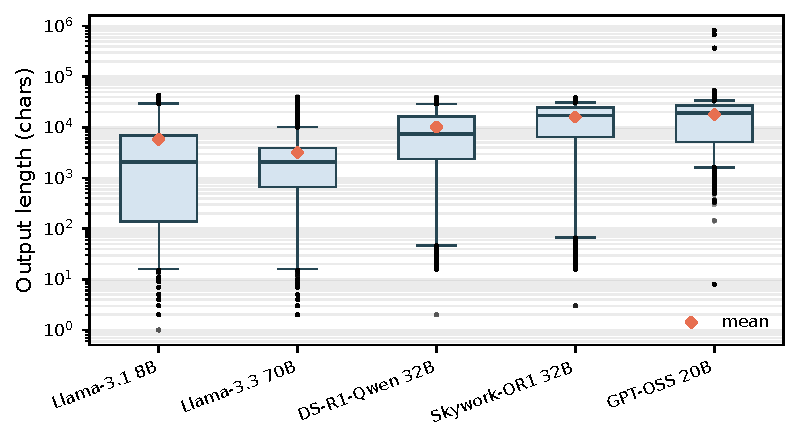
\includegraphics[width=0.6\linewidth]{figures/pdf/output_length_box.pdf}
  \caption{Output-length distribution per source LLM, in characters, pooled across every generation. Reasoning-distilled checkpoints (DS-R1-Qwen, Skywork-OR1) sit roughly an order of magnitude above the instruction-tuned Llama checkpoints at the median.}
  \label{fig:output-length}
\end{figure}

\begin{figure}[!htbp]
  \centering
  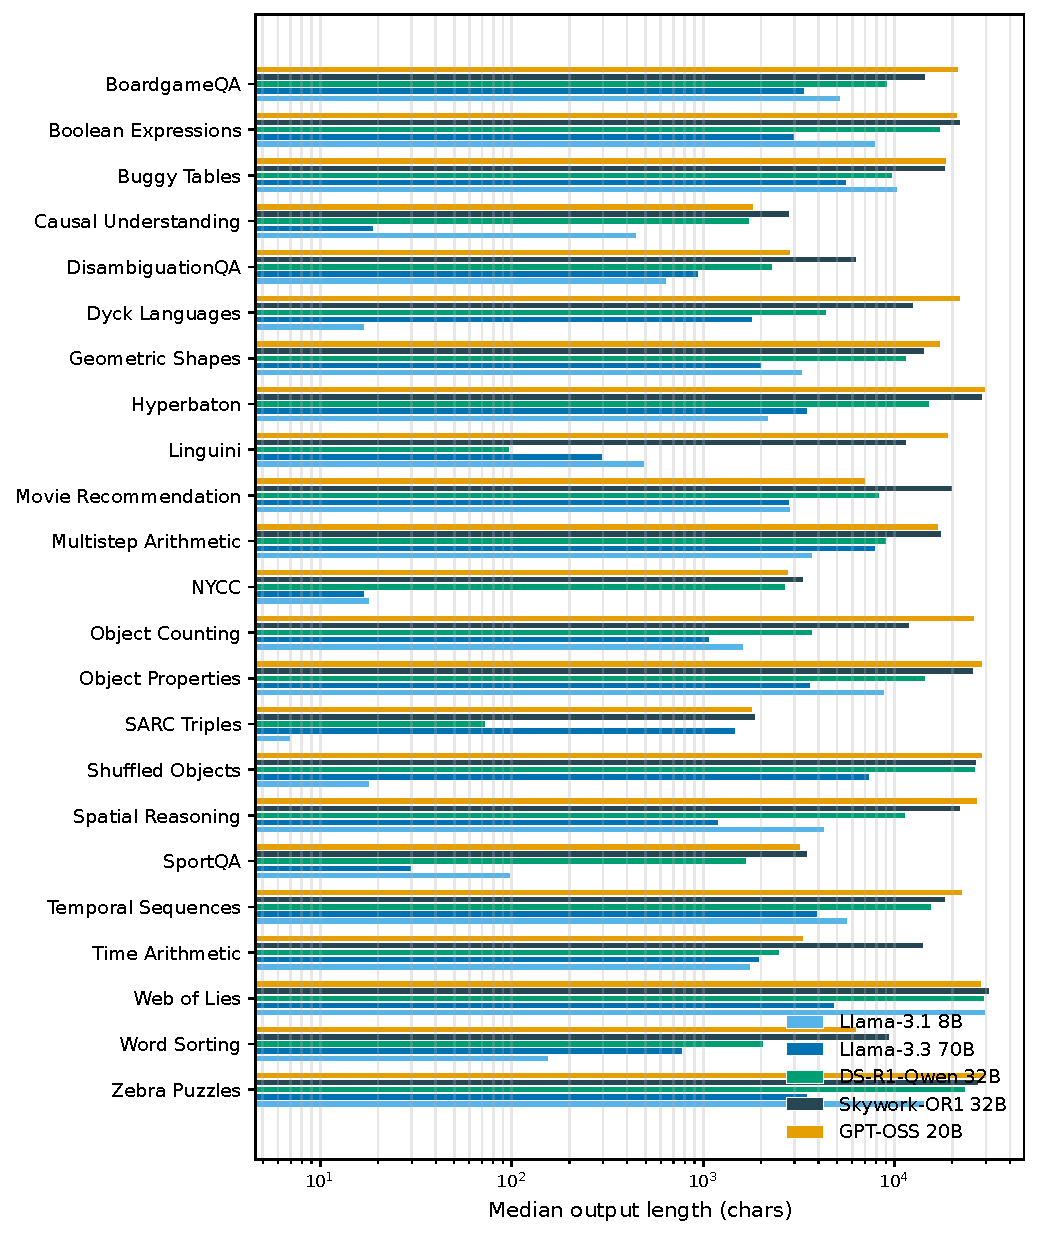
\includegraphics[width=0.85\linewidth]{figures/pdf/output_length_per_task.pdf}
  \caption{Median output length per BBEH task, in characters, with one bar per source LLM.}
  \label{fig:output-length-per-task}
\end{figure}


\subsection{BBEH Accuracy of the Source LLMs}
\label{appendix:bbeh_accuracy}

\cref{tab:bbeh-accuracy} reports BBEH correctness of the five LLMs
scored with the official extraction logic of
\citet{kazemi2025bigbenchextrahard} against the canonical task
targets. \textsc{p@1} averages correctness over all beams per problem,
while \textsc{p@8} marks a problem solved if at least one beam scores
correct, and the gap between the two columns quantifies the margin a
verifier could realise from the existing beam set. Across tasks,
Llama-3.3-70B-Instruct, Skywork-OR1-32B and GPT-OSS-20B remain ahead
of the other two on \textsc{p@1} within a few percentage points of
each other, and DS-R1-Qwen-32B records the largest \textsc{p@8} gain
relative to its own \textsc{p@1}, while GPT-OSS-20B records the
smallest such gain.

The bottom rows aggregate the per-task numbers two ways. The micro
average pools all problems across tasks, while the adjusted harmonic
mean uses the BBEH paper's aggregation $N\,/\,\sum_i 1/(a_i+1)$, which
down-weights uneven performance across tasks. For the two LLMs that
overlap with their Table~2 (Llama-3.1-8B-Instruct and DS-R1-Qwen-32B,
reported there at $3.6\%$ and $5.2\%$), our \textsc{p@1} adjusted
harmonic means agree to within the rounding granularity of the
published per-task accuracies. Llama-3.3-70B-Instruct, Skywork-OR1-32B
and GPT-OSS-20B were not evaluated under this aggregation in the
original BBEH release, so the corresponding columns extend the
benchmark's leaderboard to those checkpoints.

\begin{table}[!htbp]
  \centering
  \footnotesize
  \begin{tabular}{@{}l rr rr rr rr rr@{}}
    \toprule
     & \multicolumn{2}{c}{Llama-8B} & \multicolumn{2}{c}{Llama-70B} & \multicolumn{2}{c}{DS-R1-Qwen 32B} & \multicolumn{2}{c}{Skywork-OR1 32B} & \multicolumn{2}{c}{GPT-OSS 20B} \\
    \cmidrule(lr){2-3} \cmidrule(lr){4-5} \cmidrule(lr){6-7} \cmidrule(lr){8-9} \cmidrule(lr){10-11}
    \textbf{Task} & \textsc{p@1} & \textsc{p@8} & \textsc{p@1} & \textsc{p@8} & \textsc{p@1} & \textsc{p@8} & \textsc{p@1} & \textsc{p@8} & \textsc{p@1} & \textsc{p@8} \\
    \midrule
    BoardgameQA & 14.4 & 31.0 & 31.2 & 35.0 & 44.4 & 53.5 & 49.2 & 53.0 & 51.9 & 52.5 \\
    Boolean Expressions & 17.6 & 30.0 & 24.1 & 49.0 & 16.4 & 17.5 & 22.8 & 24.0 & 6.6 & 7.0 \\
    Buggy Tables & 0.0 & 0.0 & 0.6 & 1.5 & 0.5 & 0.5 & 1.9 & 2.5 & 7.0 & 7.0 \\
    Causal Understanding & 30.6 & 68.0 & 47.4 & 73.5 & 55.4 & 59.0 & 51.7 & 58.5 & 53.8 & 54.0 \\
    DisambiguationQA & 33.4 & 60.0 & 55.2 & 68.3 & 40.6 & 46.7 & 51.0 & 54.2 & 40.6 & 41.7 \\
    Dyck Languages & 4.1 & 32.0 & 5.9 & 16.5 & 6.8 & 7.5 & 20.7 & 21.0 & 3.6 & 4.0 \\
    Geometric Shapes & 13.5 & 26.0 & 30.4 & 51.5 & 7.6 & 11.5 & 1.5 & 1.5 & 1.0 & 2.0 \\
    Hyperbaton & 0.4 & 1.0 & 4.5 & 12.5 & 0.4 & 0.5 & 3.5 & 3.5 & 0.7 & 1.0 \\
    Linguini & 1.6 & 3.5 & 7.8 & 16.5 & 6.0 & 10.0 & 7.4 & 10.0 & 6.9 & 7.0 \\
    Movie Recommendation & 12.7 & 29.0 & 62.9 & 70.0 & 34.8 & 60.5 & 40.2 & 47.5 & 64.3 & 68.0 \\
    Multistep Arithmetic & 0.0 & 0.0 & 7.2 & 9.5 & 22.6 & 23.5 & 35.6 & 37.0 & 27.2 & 29.5 \\
    NYCC & 12.9 & 47.5 & 10.8 & 27.0 & 10.1 & 32.0 & 12.2 & 24.5 & 18.0 & 18.0 \\
    Object Counting & 0.0 & 0.0 & 14.6 & 19.5 & 3.4 & 3.5 & 9.1 & 10.0 & 0.0 & 0.0 \\
    Object Properties & 0.5 & 2.0 & 1.1 & 3.0 & 0.0 & 0.0 & 0.0 & 0.0 & 0.7 & 1.0 \\
    SARC Triples & 13.9 & 40.0 & 33.7 & 44.0 & 19.8 & 54.5 & 24.8 & 32.5 & 19.2 & 21.0 \\
    Shuffled Objects & 12.8 & 58.0 & 12.4 & 34.0 & 2.3 & 5.5 & 2.9 & 3.0 & 1.6 & 2.5 \\
    Spatial Reasoning & 5.2 & 8.5 & 11.4 & 17.0 & 14.2 & 15.0 & 16.3 & 17.5 & 0.5 & 0.5 \\
    SportQA & 2.8 & 11.5 & 15.9 & 28.0 & 23.9 & 29.0 & 24.3 & 26.5 & 17.2 & 22.5 \\
    Temporal Sequences & 0.6 & 1.5 & 2.9 & 5.5 & 4.9 & 5.0 & 0.0 & 0.0 & 0.5 & 0.5 \\
    Time Arithmetic & 5.4 & 11.5 & 30.6 & 36.5 & 42.1 & 48.5 & 48.7 & 52.0 & 70.1 & 78.0 \\
    Web of Lies & 4.2 & 8.0 & 24.3 & 29.5 & 17.6 & 18.0 & 18.3 & 18.5 & 7.0 & 8.0 \\
    Word Sorting & 3.2 & 18.0 & 20.6 & 34.5 & 25.2 & 39.5 & 33.2 & 43.0 & 46.8 & 56.0 \\
    Zebra Puzzles & 3.2 & 11.0 & 25.4 & 53.5 & 6.1 & 12.0 & 1.6 & 3.0 & 3.1 & 4.5 \\
    \midrule
    \textbf{Micro avg.} & 7.9 & 21.0 & 20.3 & 31.3 & 17.2 & 23.7 & 20.2 & 23.1 & 19.1 & 20.8 \\
    \textbf{Adj.\ HM}   & 3.1 & 4.4 & 8.7 & 15.1 & 5.5 & 6.3 & 5.3 & 5.7 & 4.0 & 4.5 \\
    \bottomrule
  \end{tabular}
\caption{BBEH accuracy (\%) per task and source LLM. \textsc{p@1} averages correctness over all beams per problem and \textsc{p@8} marks a problem solved if at least one beam scores correct. Bottom rows give the micro average across all problems and the adjusted harmonic mean $N\,/\,\sum_i 1/(a_i+1)$ over the per-task column above.}
\label{tab:bbeh-accuracy}
\end{table}


\subsection{Qualitative Beam Outputs and Embedder Similarity}
\label{appendix:beam_similarity}

To make the per-LLM beam pool concrete and to motivate why the
Output Embedding (\emph{Exact}) candidate of \cref{methodology}
captures the available semantic signal, we inspect pairs of beams from
the same input prompt and contrast a high-similarity pair against a
low-similarity pair. Cosine similarity is taken in the
Llama-Embed-Nemotron-8B space, the same space used by the Pooled and
Exact Output Embedding candidates throughout the paper. Both prompts
are drawn from the held-out test split of \cref{appendix:bbeh_accuracy}.

\begin{table}[!htbp]
\small
\centering
\begin{tabular}{p{0.47\textwidth} p{0.47\textwidth}}
\toprule
\multicolumn{2}{p{0.96\textwidth}}{\textbf{Prompt (truncated).}\
\textit{Question1\ldots If the date for the day after yesterday is
2017-12-02, what is the date 1116 days from now? Question2: A plane
leaves Location A at 01 AM UTC$+$0000 and arrives in Location B
$X'{:}Y'{:}Z'$ later. Location B is in IST(+0530). What time is it in
Location B when the plane lands?}} \\
\midrule
\textbf{Beam 1} & \textbf{Beam 2} \\
\midrule
\textit{To find the date 1116 days from 2017-12-02\ldots
$1116 \div 365 = 3$ years with a remainder of $111$\ldots
$2020$-$12$-$02 + 111$ days $= 2021$-$03$-$23$\ldots
$X' = 3$, $Y' = 24$, $Z' = 9$\ldots
UTC$+$0000\ $01{:}00{:}00 + 03{:}24{:}09 = 04{:}24{:}09 + 5\,$h
$+ 0.5\,$h $=$ UTC$+$0530\ $09{:}54{:}09$.
So, the plane lands on \underline{the same day at 09:54:09 in Location B}.
The answer is: same\_day, 09:54:09}
&
\textit{To find the date 1116 days from 2017-12-02\ldots
$1116 \div 365 = 3$ years with a remainder of $111$\ldots
$2020$-$12$-$02 + 111$ days $= 2021$-$03$-$23$\ldots
$X' = 3$, $Y' = 24$, $Z' = 9$\ldots
UTC$+$0000\ $01{:}00{:}00 + 03{:}24{:}09 = 04{:}24{:}09 + 5\,$h
$+ 0.5\,$h $=$ UTC$+$0530\ $09{:}54{:}09$.
So, the plane lands on \underline{the same day, 09:54:09}.
The answer is: same\_day, 09:54:09}
\\
\midrule
\multicolumn{2}{c}{Embedder-space cosine $\cos = 0.997$} \\
\bottomrule
\end{tabular}
\caption{High-similarity pair from example~107 of the Time Arithmetic task. Both beams
walk through the same arithmetic chain and converge on the same answer,
with only the wording of the closing sentence differing.}
\label{tab:beam_sim_high}
\end{table}

\begin{table}[!htbp]
\small
\centering
\begin{tabular}{p{0.47\textwidth} p{0.47\textwidth}}
\toprule
\multicolumn{2}{p{0.96\textwidth}}{\textbf{Prompt (truncated).}\
\textit{Jim, Carol, Bob, and Nancy share electricity from 8--9 PM. The
breaker fails if three lamps are on at the same time. Jim is not
supposed to use his lamp on Thursdays. Carol, Bob, and Nancy may use
theirs. This Thursday Jim, Carol, and Bob all turn on their lamps at
8 PM and the breaker fails. Did Jim cause the breaker to fail? Reply
Yes / No / Ambiguous.}} \\
\midrule
\textbf{Beam 2} (long-form chain of thought) & \textbf{Beam 7} (short
direct answer) \\
\midrule
\textit{To determine if Jim turning on his lamp at 8 PM caused the
circuit breaker to fail, let's analyze the situation step by step.
1.~The breaker will fail if three people turn on their lamps at the
same time. 2.~Jim is not supposed to use his lamp on Thursdays, but he
turned it on anyway. 3.~Carol and Bob also turned on their lamps at the
same time as Jim. 4.~Since Carol and Bob are allowed to use their lamps
on Thursdays, their actions did not cause the breaker to fail.
5.~The breaker failed because three people (Jim, Carol, and Bob) turned
on their lamps at the same time. Considering these points, the majority
of people would likely say that Jim turning on his lamp at 8 PM caused
the circuit breaker to fail\ldots}
&
\vspace{2em}\textit{The answer is: No.}
\\
\midrule
\textit{Verdict: \textbf{Yes} (correct)} & \textit{Verdict: \textbf{No}} \\
\midrule
\multicolumn{2}{c}{Embedder-space cosine $\cos = 0.063$} \\
\bottomrule
\end{tabular}
\caption{Low-similarity pair from example~113 of the Causal Understanding task. The
left beam walks through the rules in a multi-step argument; the right
beam returns the verdict in one line. The two beams sit in opposite
regions of the embedder space. They also disagree on the final answer:
the long-form beam concludes Yes (matching the ground truth), while the
short beam answers No.}
\label{tab:beam_sim_low}
\end{table}

The eight beams of the Causal Understanding example~113 cluster into three
regions of the embedder space. These are the long-form chain-of-thought mode and
the two short-answer modes (``Yes'' and ``No''). Within each mode,
beams sit at $\cos \ge 0.98$ from one another. Between the long-form
mode and either short mode, $\cos$ collapses to the $[0.06, 0.10]$
range regardless of whether the two beams agree on the final verdict,
so the low score in \cref{tab:beam_sim_low} is driven by format
divergence rather than answer disagreement. The showcased pair happens
to combine both format divergence and answer disagreement. The long-form beam reaches the correct answer (Yes)
while the short beam answers No, but a long-form Yes paired with a
short-form Yes would yield a cosine in the same low range. The two
short modes sit at $\cos \approx 0.80$ from each other despite
contradicting each other on the verdict. The embedder therefore
separates beams primarily by response format and only secondarily by
the content of the answer itself. This format-first geometry is what
lets the Output Embedding reach the high-purity, high-$\Delta_{\cos}$
region of \cref{appendix:geometric}, and is also why no purely latent
candidate inherits the same separation, since none of them preserves
the surface form that the embedder keys on.


\section{Broader Impacts}
\label{appendix:impact}

The work is a diagnostic protocol for representations inside frozen LLMs and produces no new generative capability, no new dataset, and no deployed system. The protocol contributes to better reasoning models and a deeper understanding of functional thought representations in LLMs. We do not identify negative societal effects of the contribution.

\section{Earlier Formulations}
\label{appendix:earlier}

\subsection{Discriminator-Based DCS Evaluation Protocol}
\label{appendix:sub:dcs_disc}

The earlier formulation of DCS reused the same-task discriminator $f_{\mathrm{disc}}$ to score within-question beam pairs.
For each test problem $x$ with $K=8$ beams, two variants of the semantic equivalence matrix were constructed.
$\mathbf{E}^{\mathrm{emb}} \in \{0,1\}^{K \times K}$ sets $\mathbf{E}^{\mathrm{emb}}_{ij} = 1$ when the cosine similarity between the Nemotron embeddings of $y_i$ and $y_j$ exceeds $\tau = 0.9$, and $0$ otherwise.
$\mathbf{E}^{\mathrm{parse}} \in \{0,1\}^{K \times K}$ sets $\mathbf{E}^{\mathrm{parse}}_{ij} = 1$ when the extracted final answers from $y_i$ and $y_j$ match exactly using the official BBEH answer extraction logic~\citep{kazemi2025bigbenchextrahard}, with beam pairs for which either side has no extractable answer excluded rather than labelled non-equivalent.
The functional similarity matrix $\mathbf{M} \in [0,1]^{K \times K}$ was defined by the symmetric cross score $\mathbf{M}_{ij} = \tfrac{1}{2}(f_{\mathrm{disc}}(\mathbf{T}_i, y_j) + f_{\mathrm{disc}}(\mathbf{T}_j, y_i))$, and the score was the inverse mean absolute error between $\mathbf{M}$ and $\mathbf{E}$ over off-diagonal pairs,
\begin{equation}\label{eq:dcs-disc-earlier}
    \mathrm{DCS}_{\mathrm{disc}}(x) = 1 - \frac{1}{K(K-1)}\sum_{i}\sum_{j \neq i} \bigl|\mathbf{M}_{ij} - \mathbf{E}_{ij}\bigr|.
\end{equation}
This formulation proved uninformative in practice.
The discriminator was trained on cross-question pairs and provided no gradient signal for within-question scoring, so $f_{\mathrm{disc}}$ returned values near $0.5$ for all same-question beam pairs.
This collapsed $\mathrm{DCS}_{\mathrm{disc}}$ to the random baseline for every representation family and source LLM (see \cref{tab:dcs}).

\subsection{Causality with the Discriminator-Trained Projection}
\label{appendix:sub:causality_disc_proj}

\cref{tab:causality-disc} reports the causality KL under the discriminator-trained projection of \cref{appendix:sub:disc_arch}. This was the projection used in our first iteration of the causality protocol, before the projection-swap pilot of \cref{appendix:sub:causality_minproj} motivated adopting the output-reconstruction projection in \cref{tab:causality-results}. The earlier table is retained so that the effect of the projection swap remains visible cell-by-cell against the current results. Without length normalisation and under the discriminator-trained projection, several causality values are not well calibrated. Random vectors receive lower causality scores than expected because the model can ignore an uninformative input and produce whatever is more aligned with the output. Several other candidate representations produce higher causality than the random vector, which contradicts the behavioural reading the metric should provide.

% Legacy headline causality. Cells display the mean KL(Z | T) with its
% marginal bootstrap SE under the discriminator-trained projection of
% \cref{appendix:sub:disc_arch}. Retained for cell-by-cell comparison
% against the headline (\cref{tab:causality-results}).

\begin{table}[!htbp]
  \centering
  \footnotesize
  \setlength{\tabcolsep}{2.5pt}
  \renewcommand{\arraystretch}{1.1}
  \resizebox{\textwidth}{!}{%
  \begin{tabular}{@{}l *{2}{c} !{\vrule} *{2}{c} *{5}{c} *{5}{c} *{5}{c} !{\vrule} *{2}{c}@{}}
    \toprule
    & \multicolumn{2}{c}{\textit{Output Emb.}}
      & \multicolumn{2}{c}{\textit{Last Input Tok.}}
      & \multicolumn{5}{c}{\textit{Soft Thinking (no noise)}}
      & \multicolumn{5}{c}{\textit{Soft Thinking (Gumbel)}}
      & \multicolumn{5}{c}{\textit{Latent Thinking}}
      & \multicolumn{2}{c}{\textit{Baselines}} \\
    \cmidrule(lr){2-3}\cmidrule(lr){4-5}\cmidrule(lr){6-10}\cmidrule(lr){11-15}\cmidrule(lr){16-20}\cmidrule(lr){21-22}
    \textbf{LLM}
      & Exc & Pool
      & All & Final
      & 1 & 16 & 32 & 64 & 128
      & 1 & 16 & 32 & 64 & 128
      & 1 & 16 & 32 & 64 & 128
      & IE & RV \\
    \midrule
    Llama-3.1 8B     & \ciAdvNS{4.89}{0.09} & \ciAdvNS{4.69}{0.09} & \ciAdvNS{6.13}{0.06} & \ciAdvNS{4.52}{0.07} & \ciAdvNS{4.43}{0.06} & \ciAdvNS{5.83}{0.08} & \ciAdvNS{9.31}{0.09} & \ciAdvNS{8.93}{0.08} & \ciAdvNS{7.31}{0.08} & \ciAdvNS{4.96}{0.08} & \ciAdvNS{7.46}{0.16} & \ciAdvNS{7.94}{0.10} & \ciAdvNS{8.40}{0.08} & \ciAdvNS{7.15}{0.06} & \ciAdvInf{4.21}{0.07} & \ciAdvNS{8.06}{0.08} & \ciAdvNS{4.37}{0.09} & \ciAdvNS{9.81}{0.09} & \ciAdvNS{8.14}{0.10} & \ciAdvNS{7.46}{0.13} & \ciSE{4.48}{0.07} \\
    Llama-3.3 70B    & \ciAdvNS{4.90}{0.08} & \ciAdvNS{8.45}{0.06} & \ciAdvNS{7.41}{0.07} & \ciAdvNS{10.36}{0.04} & \ciAdvNSB{4.85}{0.09} & \ciAdvNS{9.34}{0.07} & \ciAdvNS{7.69}{0.05} & \ciAdvNS{9.61}{0.09} & \ciAdvNS{10.51}{0.07} & \ciAdvNS{5.84}{0.07} & \ciAdvNS{6.93}{0.08} & \ciAdvNS{10.27}{0.12} & \ciAdvNS{7.18}{0.06} & \ciAdvNS{8.53}{0.05} & \ciAdvNS{6.85}{0.06} & \ciAdvNS{8.99}{0.05} & \ciAdvNS{9.47}{0.05} & \ciAdvNS{8.09}{0.05} & \ciAdvNS{9.52}{0.05} & \ciAdvNS{4.54}{0.12} & \ciSE{4.44}{0.05} \\
    DS-R1-Qwen 32B  & \ciAdvNS{4.60}{0.08} & \ciAdvNS{4.81}{0.07} & \ciAdvNS{9.21}{0.06} & \ciAdvNS{9.18}{0.08} & \ciAdvNS{7.01}{0.08} & \ciAdvNS{6.20}{0.06} & \ciAdvNS{7.24}{0.07} & \ciAdvNS{9.20}{0.07} & \ciAdvNS{7.74}{0.08} & \ciAdvNS{8.15}{0.13} & \ciAdvNS{7.42}{0.06} & \ciAdvNS{6.83}{0.06} & \ciAdvNS{8.90}{0.07} & \ciAdvNS{7.34}{0.05} & \ciAdvNSB{4.74}{0.06} & \ciAdvNS{5.52}{0.06} & \ciAdvNS{9.55}{0.09} & \ciAdvNS{7.67}{0.06} & \ciAdvNS{8.02}{0.06} & \ciAdvNS{6.56}{0.11} & \ciSE{4.54}{0.06} \\
    \bottomrule
  \end{tabular}%
  }
\caption{Causality KL ($\downarrow$) across source LLMs under the discriminator-trained projection of \cref{appendix:sub:disc_arch}. The discriminator dataset expands single-vector representations to a common training length and repeats shorter multi-vector representations to that same length, so the projection itself is learned at fixed length and is internally consistent with feeding $\mathbf{T}$ at the same length here.}
\label{tab:causality-disc}
\end{table}


\subsection{Cross-Entropy Proxy for Minimality}
\label{appendix:minimality-components}

The minimality formulation we initially proposed approximated the IB Lagrangian as a single cross-entropy gap $\Delta_{\text{CE}} = \text{CE}(X \mid \mathbf{T}) - \text{CE}(Y \mid \mathbf{T})$, on the intuition that a high gap reflects a representation that compresses the input while retaining output-relevant information. We retain that analysis here for transparency. Two issues motivated the corrected formulation $\Delta_{\text{IB}}$ adopted in \cref{methodology} and derived in \cref{appendix:sub:minimality_ib_derivation}. First, $\Delta_{\text{CE}}$ corresponds to the IB Lagrangian only at the trade-off weight $\beta = 1$, where the chain-rule decomposition cancels the sufficiency reward and leaves only the redundancy penalty $-I(X; \mathbf{T} \mid Y)$, so the metric is unbalanced before any empirical concern. Second, the input-reconstruction probe $\text{CE}(X \mid \mathbf{T})$ saturates uniformly across representations because no probe in our class can reconstruct the exact lexical phrasing of $X$ from any latent $\mathbf{T}$, which collapses the gap into a function of $\text{CE}(Y \mid \mathbf{T})$ alone. The corrected $\Delta_{\text{IB}}$ replaces $\text{CE}(X \mid \mathbf{T})$ with the conditional $\text{CE}(X \mid Y, \mathbf{T})$, which estimates the residual mutual information $I(X; \mathbf{T} \mid Y)$ and does not saturate. The components reported below corroborate the saturation diagnosis on every source model.

A high $\Delta_{\text{CE}}$ driven by high $\text{CE}(X \mid \mathbf{T})$ (input compression) and low $\text{CE}(Y \mid \mathbf{T})$ (output retention) would reflect a minimal sufficient $\mathbf{T}$, whereas a high gap produced by both conditionals drifting upward reflects a $\mathbf{T}$ that has lost information about both $X$ and $Y$. \cref{tab:minimality-ce-x} reports the input component per source LLM, and \cref{tab:minimality-ce-y} reports the output component. The Random Vector anchor for the input probe converges to $\text{CE}(X \mid \mathrm{RV}) \approx 1.87 \pm 0.04$ on every source LLM, since the probe sees the same input distribution and i.i.d.\ noise regardless of which model produced the candidates, so the column is omitted from \cref{tab:minimality-ce-x} and reported once here. Every Llama-3.1-8B cell of $\text{CE}(X \mid \mathbf{T})$ has a CI that overlaps this anchor, so the input component alone does not discriminate among candidates on this model. The output component does separate $\mathrm{RV}$ from every other candidate, since the Random Vector $\text{CE}(Y \mid \mathbf{T})$ is above the upper CI bound of every non-RV cell.

The two anchor candidates make the rest of the table interpretable. The Output Embedding (\emph{Exact}) achieves the lowest CE$(Y \mid \mathbf{T})$ on Llama-3.1-8B, since the probe is being asked to predict $Y$ from a representation of $Y$ itself, and the Pooled variant follows behind with the per-beam information collapsed away. The Input Embedding is at the centre of the candidate cloud, since the input prompt alone determines the high-probability output and a probe over its embedding can already predict $Y$ before any latent computation has happened. Any candidate above the Input Embedding's CE$(Y \mid \mathbf{T})$ has drifted away from the input without acquiring additional $Y$-relevant content, while any candidate below it has packed in further output-relevant information beyond what the prompt already carries.

The same anchor reading carries to the implied gap. Subtracting the two components above on Llama-3.1-8B places the Input Embedding's $\Delta_{\text{CE}}$ already in the high $0.9$ range, so the prompt itself, before any latent computation, already exhibits the minimality profile that a thought representation is supposed to provide. Most thinking candidates land at or below that input-alone gap, and only the Output Embedding (\emph{Exact}) clearly exceeds it. The proxy therefore separates Random Vector from the rest of the field, but it also reports that latent thinking does not produce a more compressed, output-relevant summary of the problem than directly embedding the input prompt.

% Minimality components: input-reconstruction cross-entropy
% $\text{CE}(X \mid \mathbf{T})$ and output-prediction cross-entropy
% $\text{CE}(Y \mid \mathbf{T})$ per source LLM. The headline Minimality Gap
% $\Delta_{\text{CE}}$ derived from these components is reported in
% \cref{tab:minimality-delta-ce}.

\begin{table}[!htbp]
  \centering
  \footnotesize
  \setlength{\tabcolsep}{2.5pt}
  \renewcommand{\arraystretch}{1.1}
  \resizebox{\textwidth}{!}{%
  \begin{tabular}{@{}l *{2}{c} !{\vrule} *{2}{c} *{5}{c} *{5}{c} *{5}{c} !{\vrule} c@{}}
    \toprule
    & \multicolumn{2}{c}{\textit{Output Emb.}}
      & \multicolumn{2}{c}{\textit{Last Input Tok.}}
      & \multicolumn{5}{c}{\textit{Soft Thinking (no noise)}}
      & \multicolumn{5}{c}{\textit{Soft Thinking (Gumbel)}}
      & \multicolumn{5}{c}{\textit{Latent Thinking}}
      & \textit{Baseline} \\
    \cmidrule(lr){2-3}\cmidrule(lr){4-5}\cmidrule(lr){6-10}\cmidrule(lr){11-15}\cmidrule(lr){16-20}\cmidrule(lr){21-21}
    \textbf{LLM}
      & Exc & Pool
      & All & Final
      & 1 & 16 & 32 & 64 & 128
      & 1 & 16 & 32 & 64 & 128
      & 1 & 16 & 32 & 64 & 128
      & IE \\
    \midrule
    Llama-3.1 8B     & \ciSE{1.77}{0.04} & \ciSE{1.78}{0.04} & \ciSE{1.74}{0.04} & \ciSE{1.75}{0.04} & \ciSE{1.74}{0.04} & \ciSE{1.74}{0.04} & \ciSE{1.75}{0.04} & \ciSE{1.77}{0.04} & \ciSE{1.78}{0.04} & \ciSE{1.75}{0.04} & \ciSE{1.75}{0.04} & \ciSE{1.76}{0.04} & \ciSE{1.77}{0.04} & \ciSE{1.78}{0.04} & \ciSE{1.74}{0.04} & \ciSE{1.74}{0.04} & \ciSE{1.75}{0.04} & \ciSE{1.76}{0.04} & \ciSE{1.76}{0.04} & \ciSE{1.78}{0.04} \\
    Llama-3.3 70B    & \ciSE{1.75}{0.04} & \ciSE{1.77}{0.04} & \ciSE{1.70}{0.04} & \ciSE{1.73}{0.04} & \ciSE{1.74}{0.04} & \ciSE{1.69}{0.04} & \ciSE{1.72}{0.04} & \ciSE{1.74}{0.04} & \ciSE{1.76}{0.04} & \ciSE{1.74}{0.04} & \ciSE{1.72}{0.04} & \ciSE{1.74}{0.04} & \ciSE{1.75}{0.04} & \ciSE{1.76}{0.04} & \ciSE{1.72}{0.04} & \ciSE{1.72}{0.04} & \ciSE{1.73}{0.04} & \ciSE{1.73}{0.04} & \ciSE{1.74}{0.04} & \ciSE{1.78}{0.04} \\
    DS-R1-Qwen 32B  & \ciSE{1.75}{0.04} & \ciSE{1.78}{0.04} & \ciSE{1.73}{0.04} & \ciSE{1.74}{0.04} & \ciSE{1.74}{0.04} & \ciSE{1.75}{0.04} & \ciSE{1.76}{0.04} & \ciSE{1.78}{0.04} & \ciSE{1.80}{0.04} & \ciSE{1.75}{0.04} & \ciSE{1.78}{0.04} & \ciSE{1.78}{0.04} & \ciSE{1.79}{0.04} & \ciSE{1.81}{0.04} & \ciSE{1.73}{0.04} & \ciSE{1.72}{0.04} & \ciSE{1.73}{0.04} & \ciSE{1.74}{0.04} & \ciSE{1.75}{0.04} & \ciSE{1.78}{0.04} \\
    \bottomrule
  \end{tabular}%
  }
\caption{Input-reconstruction cross-entropy $\text{CE}(X \mid \mathbf{T})$ across source LLMs. Higher values indicate that $\mathbf{T}$ carries less information about the input prompt. The Random Vector baseline is omitted because the probe sees the same $X$ and i.i.d.\ noise on every source LLM, so $\text{CE}(X \mid \mathrm{RV}) \approx 1.87$ uniformly and serves as a single shared anchor referenced in the surrounding prose.}
\label{tab:minimality-ce-x}
\end{table}

\begin{table}[!htbp]
  \centering
  \footnotesize
  \setlength{\tabcolsep}{2.5pt}
  \renewcommand{\arraystretch}{1.1}
  \resizebox{\textwidth}{!}{%
  \begin{tabular}{@{}l *{2}{c} !{\vrule} *{2}{c} *{5}{c} *{5}{c} *{5}{c} !{\vrule} *{2}{c}@{}}
    \toprule
    & \multicolumn{2}{c}{\textit{Output Emb.}}
      & \multicolumn{2}{c}{\textit{Last Input Tok.}}
      & \multicolumn{5}{c}{\textit{Soft Thinking (no noise)}}
      & \multicolumn{5}{c}{\textit{Soft Thinking (Gumbel)}}
      & \multicolumn{5}{c}{\textit{Latent Thinking}}
      & \multicolumn{2}{c}{\textit{Baselines}} \\
    \cmidrule(lr){2-3}\cmidrule(lr){4-5}\cmidrule(lr){6-10}\cmidrule(lr){11-15}\cmidrule(lr){16-20}\cmidrule(lr){21-22}
    \textbf{LLM}
      & Exc & Pool
      & All & Final
      & 1 & 16 & 32 & 64 & 128
      & 1 & 16 & 32 & 64 & 128
      & 1 & 16 & 32 & 64 & 128
      & IE & RV \\
    \midrule
    Llama-3.1 8B     & \ciSE{0.77}{0.03} & \ciSE{0.84}{0.02} & \ciSE{0.78}{0.02} & \ciSE{0.81}{0.02} & \ciSE{0.85}{0.03} & \ciSE{0.82}{0.02} & \ciSE{0.84}{0.02} & \ciSE{0.86}{0.02} & \ciSE{0.83}{0.03} & \ciSE{0.89}{0.03} & \ciSE{0.84}{0.03} & \ciSE{0.88}{0.02} & \ciSE{0.88}{0.02} & \ciSE{0.90}{0.03} & \ciSE{0.83}{0.02} & \ciSE{0.78}{0.02} & \ciSE{0.79}{0.02} & \ciSE{0.80}{0.02} & \ciSE{0.82}{0.02} & \ciSE{0.83}{0.02} & \ciSE{1.91}{0.08} \\
    Llama-3.3 70B    & \ciSE{1.25}{0.03} & \ciSE{1.31}{0.03} & \ciSE{1.16}{0.03} & \ciSE{1.22}{0.03} & \ciSE{1.38}{0.03} & \ciSE{1.21}{0.03} & \ciSE{1.23}{0.03} & \ciSE{1.25}{0.03} & \ciSE{1.25}{0.03} & \ciSE{1.39}{0.03} & \ciSE{1.24}{0.03} & \ciSE{1.27}{0.03} & \ciSE{1.28}{0.03} & \ciSE{1.27}{0.03} & \ciSE{1.28}{0.03} & \ciSE{1.24}{0.03} & \ciSE{1.25}{0.03} & \ciSE{1.27}{0.03} & \ciSE{1.29}{0.03} & \ciSE{1.35}{0.03} & \ciSE{2.35}{0.07} \\
    DS-R1-Qwen 32B  & \ciSE{0.83}{0.03} & \ciSE{0.86}{0.03} & \ciSE{0.76}{0.02} & \ciSE{0.78}{0.02} & \ciSE{0.83}{0.03} & \ciSE{0.82}{0.03} & \ciSE{0.83}{0.03} & \ciSE{0.87}{0.03} & \ciSE{0.89}{0.03} & \ciSE{0.86}{0.03} & \ciSE{0.89}{0.03} & \ciSE{0.87}{0.03} & \ciSE{0.88}{0.03} & \ciSE{0.89}{0.03} & \ciSE{0.82}{0.02} & \ciSE{0.83}{0.03} & \ciSE{0.84}{0.03} & \ciSE{0.86}{0.03} & \ciSE{0.87}{0.03} & \ciSE{0.91}{0.03} & \ciSE{1.33}{0.05} \\
    \bottomrule
  \end{tabular}%
  }
\caption{Output-prediction cross-entropy $\text{CE}(Y \mid \mathbf{T})$ across source LLMs at each representation's native sequence length. Lower values indicate that $\mathbf{T}$ retains information sufficient to predict the output sequence. The tiled-length companion in \cref{tab:minimality-ce-y-tiled} reports the same quantity with every representation fed at a common length, isolating the effect of length normalisation.}
\label{tab:minimality-ce-y}
\end{table}

% The tiled-length companion of CE(Y|T) is in
% \cref{tab:minimality-ce-y-tiled}, paired with the conditional input
% probe CE(X|Y,T) in \cref{tab:minimality-ce-xyt-tiled}; both live with
% the IB-residual headline (\cref{tab:minimality-delta-ib}) in the
% main appendix.


\subsection{Qualitative Probe Reconstruction}
\label{appendix:qualitative_probe}

\cref{tab:probe_reconstruction} shows a concrete example of input probe
reconstruction failure. Given the Last Input Token thought representation
$\mathbf{T}$ extracted from a BoardGame QA problem (a multi-step logical deduction
task from BBEH), the input probe (a linear projection followed by a frozen
LLaMA-3.2-1B) attempts to reconstruct the original input sequence $X$.

\begin{table}[!htbp]
\small
\begin{tabular}{p{0.47\textwidth} p{0.47\textwidth}}
\toprule
\textbf{Reference Input $X$ (truncated)} & \textbf{Probe Prediction $\hat{X}$ given $\mathbf{T}$} \\
\midrule
\textit{A few players are playing a boardgame. The current state of the game
is as follows. The akita is watching a movie from 1974. The akita is a high
school teacher. The dove has a football with a radius of 30 inches. The elk is
3 years old. The german shepherd unites with the ant. [\ldots] And the rules of
the game are as follows. Rule1: \ldots Rule2: \ldots Rule3: \ldots}
&
\textit{Question: Which of the following is not a valid argument for the claim
that the number of people who are not in the United States is greater than the
number of people who are in the United States?\newline
A. The number of people who are in the United States is greater than \ldots\newline
B. \ldots\newline
C. \ldots\newline
D. \ldots\newline
Answer: D}
\\
\bottomrule
\end{tabular}
\caption{Qualitative example of input probe reconstruction failure.
The probe is conditioned on the Last Input Token thought representation
($\Delta_{\mathrm{CE}} = 0.18$, $\mathrm{CE}(X|\mathbf{T}) = 1.63$).
All 10 sampled problems from this task produce the same boilerplate prediction.}
\label{tab:probe_reconstruction}
\end{table}

Crucially, all 10 sampled BoardGame QA problems yield the same
boilerplate prediction, namely a multiple-choice question about a completely unrelated
topic. This indicates that the thought representation $\mathbf{T}$ has discarded
all problem-specific content. The probe has learned to output a domain-generic
template (plausible given the BBEH multiple-choice format) rather than
recovering any instance-specific detail. This qualitatively confirms the
same-task separability collapse. If the probe cannot distinguish between 10
different board game problems when conditioned on $\mathbf{T}$, neither can
the same-task discriminator.

\subsection{Discriminator-Based DCS Results}
\label{appendix:sub:dcs_disc_results}

The discriminator-based DCS formulation and its failure mode are documented in \cref{appendix:sub:dcs_disc}.
The results below retain that analysis for transparency.

\cref{fig:dcs-emb-vs-parse} (top row) plots discriminator-based DCS under $\mathbf{E}_{\text{parse}}$ against the same score under $\mathbf{E}_{\text{emb}}$ for every representation, one panel per source model.
The two variants agree closely on every model, so the table reports $\mathbf{E}_{\text{emb}}$.
On Llama-3.3-70B-Instruct every representation crowds near $0.5$, so the linear correlation collapses to noise even though the absolute disagreement remains small.
$\mathbf{E}_{\text{emb}}$ also remains defined on beams where BBEH answer extraction fails (see \cref{appendix:dataset}).

\cref{fig:dcs-emb-vs-parse} (bottom row) shows the cosine-similarity distribution over off-diagonal beam pairs.
The distribution is bimodal on every model, with a large right mode near $1$ accounting for paraphrase-equivalent pairs and a small left mode below $0.5$ for genuine cross-answer pairs.

\begin{figure}[t]
  \centering
  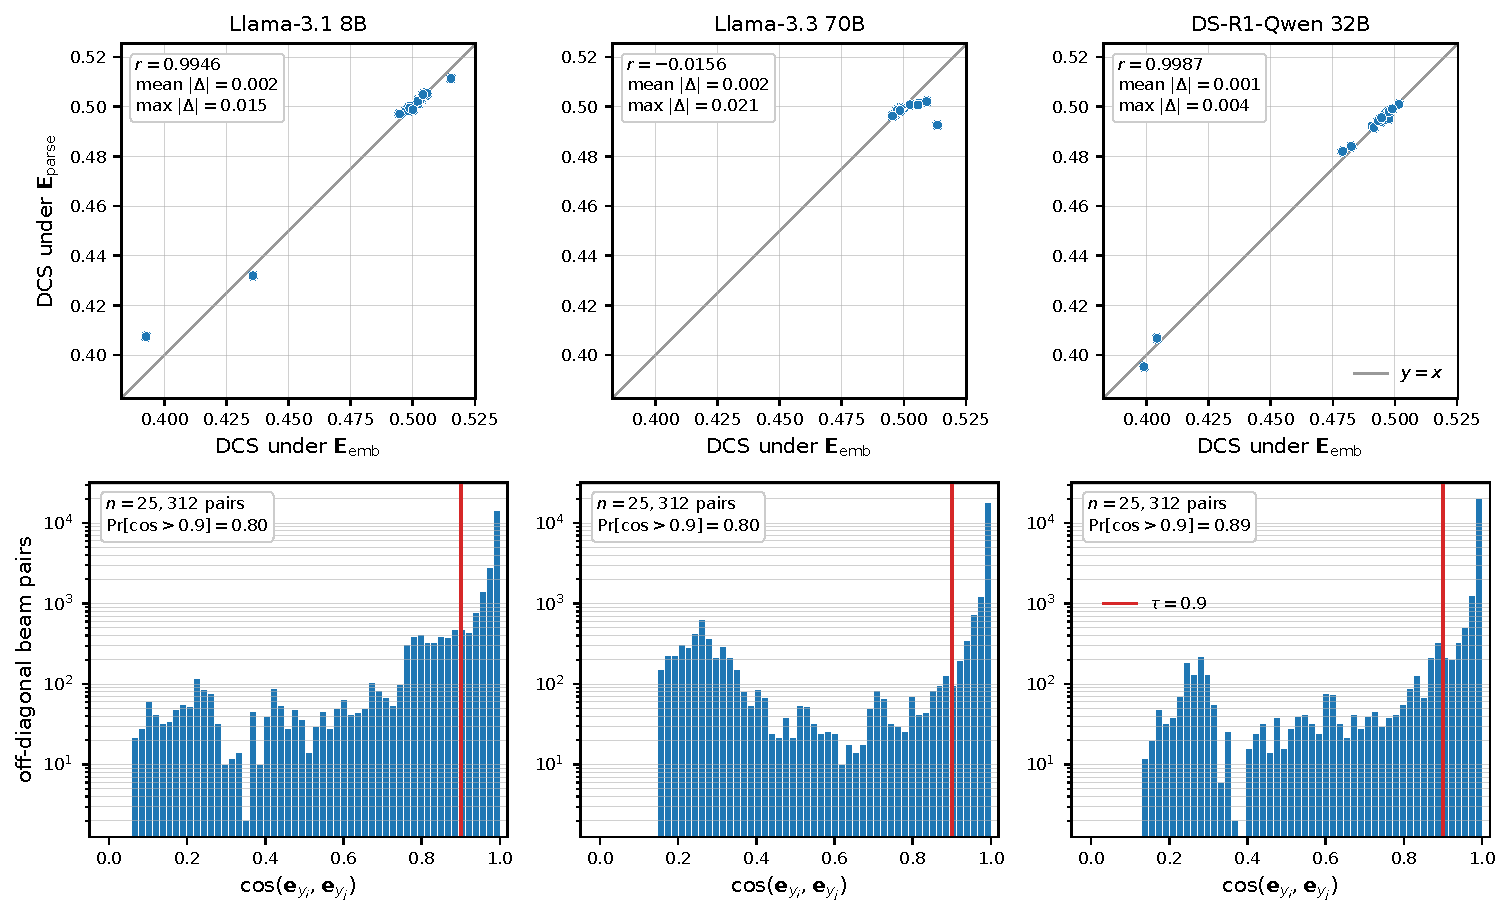
\includegraphics[width=\linewidth]{figures/pdf/dcs_emb_vs_parse.pdf}
  \caption{Discriminator-based DCS. The top row shows the score under $\mathbf{E}_{\text{parse}}$ against the same score under $\mathbf{E}_{\text{emb}}$ for every representation, one panel per source model. The bottom row shows the empirical distribution of off-diagonal pairwise beam cosine similarities, one panel per source model, with the threshold $\tau{=}0.9$ overlaid.}
  \label{fig:dcs-emb-vs-parse}
\end{figure}


% DCS per source LLM under E_emb (E_parse agreement shown in figure).
% Transposed layout matching main-text convention in tables/disc_results.tex.

\begin{table}[!htbp]
  \centering
  \footnotesize
  \setlength{\tabcolsep}{2.5pt}
  \renewcommand{\arraystretch}{1.1}
  \resizebox{\textwidth}{!}{%
  \begin{tabular}{@{}l *{2}{c} !{\vrule} *{2}{c} *{5}{c} *{5}{c} *{5}{c} !{\vrule} *{2}{c}@{}}
    \toprule
    & \multicolumn{2}{c}{\textit{Output Emb.}}
      & \multicolumn{2}{c}{\textit{Last Input Tok.}}
      & \multicolumn{5}{c}{\textit{Soft Thinking (no noise)}}
      & \multicolumn{5}{c}{\textit{Soft Thinking (Gumbel)}}
      & \multicolumn{5}{c}{\textit{Latent Thinking}}
      & \multicolumn{2}{c}{\textit{Baselines}} \\
    \cmidrule(lr){2-3}\cmidrule(lr){4-5}\cmidrule(lr){6-10}\cmidrule(lr){11-15}\cmidrule(lr){16-20}\cmidrule(lr){21-22}
    \textbf{LLM}
      & Exc & Pool
      & All & Final
      & 1 & 16 & 32 & 64 & 128
      & 1 & 16 & 32 & 64 & 128
      & 1 & 16 & 32 & 64 & 128
      & IE & RV \\
    \midrule
    Llama-3.1 8B    & \ciAdvNS{0.393}{0.012} & \ciAdvNS{0.436}{0.010} & \ciAdvInf{0.505}{0.001} & \ciAdvNS{0.499}{0.002} & \ciAdvInf{0.502}{0.001} & \ciAdvInf{0.504}{0.001} & \ciAdvInfB{0.515}{0.002} & \ciAdvInf{0.506}{0.002} & \ciAdvInf{0.502}{0.001} & \ciAdvNS{0.502}{0.001} & \ciAdvInf{0.503}{0.001} & \ciAdvInf{0.504}{0.001} & \ciAdvNS{0.500}{0.001} & \ciAdvNS{0.499}{0.000} & \ciAdvInf{0.505}{0.002} & \ciAdvNS{0.499}{0.001} & \ciAdvNS{0.495}{0.001} & \ciAdvNS{0.498}{0.001} & \ciAdvNS{0.497}{0.001} & \ciAdvNS{0.498}{0.003} & \ciAdvNS{0.499}{0.001} \\
    Llama-3.3 70B   & \ciAdvNS{0.514}{0.012} & \ciAdvInf{0.506}{0.001} & \ciAdvNS{0.500}{0.001} & \ciAdvNS{0.498}{0.000} & \ciAdvInf{0.509}{0.001} & \ciAdvInf{0.502}{0.001} & \ciAdvNS{0.499}{0.000} & \ciAdvNS{0.497}{0.001} & \ciAdvNS{0.498}{0.000} & \ciAdvInf{0.506}{0.001} & \ciAdvInf{0.503}{0.000} & \ciAdvNS{0.495}{0.001} & \ciAdvNS{0.498}{0.001} & \ciAdvNS{0.497}{0.000} & \ciAdvNS{0.498}{0.000} & \ciAdvNS{0.498}{0.000} & \ciAdvNS{0.498}{0.001} & \ciAdvNS{0.498}{0.000} & \ciAdvNS{0.498}{0.000} & \ciAdvNS{0.499}{0.001} & \ciSE{0.498}{0.001} \\
    DS-R1-Qwen 32B & \ciAdvNS{0.399}{0.010} & \ciAdvNS{0.404}{0.010} & \ciAdvInfB{0.502}{0.000} & \ciAdvNS{0.496}{0.001} & \ciAdvNS{0.498}{0.001} & \ciAdvNS{0.492}{0.003} & \ciAdvNS{0.482}{0.004} & \ciAdvNS{0.494}{0.003} & \ciAdvNS{0.496}{0.002} & \ciAdvNS{0.499}{0.001} & \ciAdvNS{0.498}{0.001} & \ciAdvNS{0.493}{0.001} & \ciAdvNS{0.495}{0.001} & \ciAdvNS{0.495}{0.000} & \ciAdvNS{0.496}{0.000} & \ciAdvNS{0.497}{0.000} & \ciAdvNS{0.491}{0.001} & \ciAdvNS{0.496}{0.000} & \ciAdvNS{0.497}{0.000} & \ciAdvNS{0.479}{0.005} & \ciSE{0.497}{0.001} \\
    \bottomrule
  \end{tabular}%
  }
\caption{Discriminator-based DCS under $\mathbf{E}_{\mathrm{emb}}$ ($\tau{=}0.9$, $\uparrow$) across source LLMs, using the formulation documented in \cref{appendix:sub:dcs_disc}. Values near $0.5$ across representations reflect discriminator saturation on within-question pairs.}
\label{tab:dcs}
\end{table}


\cref{tab:dcs-tau-sweep} sweeps the cosine-similarity threshold $\tau$ on Llama-3.1-8B-Instruct.
All rows share the same test split, trained discriminator, and beam embeddings.
Only the binarisation $\mathbf{E}_{\mathrm{emb}}^{ij} = \mathbb{1}[\cos(y_i, y_j) > \tau]$ varies.
The ranking is stable across the full range and the chance-floor cluster does not reshuffle at any threshold, confirming that the saturation is intrinsic to the discriminator-based scoring and not an artefact of the threshold choice.

% DCS under E_emb swept across six cosine-similarity thresholds tau.
% Rows: tau in {0.60, 0.70, 0.80, 0.85, 0.90, 0.95}. Columns mirror
% tables/dcs_res.tex. Cells are plain black (\ciSE) since this table
% reports sensitivity, not the informative-vs-chance verdict. Values
% are recomputed offline from the cos_sim and M matrices cached in the
% main DCS run, so the tau=0.90 row reproduces tables/dcs_res.tex
% cell-for-cell.

\begin{table}[!htbp]
  \centering
  \footnotesize
  \setlength{\tabcolsep}{2.5pt}
  \renewcommand{\arraystretch}{1.1}
  \resizebox{\textwidth}{!}{%
  \begin{tabular}{@{}l *{2}{c} !{\vrule} *{2}{c} *{5}{c} *{5}{c} *{5}{c} !{\vrule} *{2}{c}@{}}
    \toprule
    & \multicolumn{2}{c}{\textit{Output Emb.}}
      & \multicolumn{2}{c}{\textit{Last Input Tok.}}
      & \multicolumn{5}{c}{\textit{Soft Thinking (no noise)}}
      & \multicolumn{5}{c}{\textit{Soft Thinking (Gumbel)}}
      & \multicolumn{5}{c}{\textit{Latent Thinking}}
      & \multicolumn{2}{c}{\textit{Baselines}} \\
    \cmidrule(lr){2-3}\cmidrule(lr){4-5}\cmidrule(lr){6-10}\cmidrule(lr){11-15}\cmidrule(lr){16-20}\cmidrule(lr){21-22}
    $\boldsymbol{\tau}$
      & Exc & Pool
      & All & Final
      & 1 & 16 & 32 & 64 & 128
      & 1 & 16 & 32 & 64 & 128
      & 1 & 16 & 32 & 64 & 128
      & IE & RV \\
    \midrule
    $0.60$ & \ciSE{0.385}{0.012} & \ciSE{0.438}{0.010} & \ciSE{0.509}{0.001} & \ciSE{0.496}{0.002} & \ciSE{0.510}{0.001} & \ciSE{0.506}{0.001} & \ciSE{0.516}{0.003} & \ciSE{0.507}{0.002} & \ciSE{0.501}{0.001} & \ciSE{0.504}{0.001} & \ciSE{0.502}{0.001} & \ciSE{0.501}{0.001} & \ciSE{0.505}{0.001} & \ciSE{0.498}{0.000} & \ciSE{0.503}{0.002} & \ciSE{0.500}{0.001} & \ciSE{0.496}{0.002} & \ciSE{0.499}{0.001} & \ciSE{0.496}{0.001} & \ciSE{0.499}{0.003} & \ciSE{0.496}{0.001} \\
    $0.70$ & \ciSE{0.387}{0.012} & \ciSE{0.437}{0.010} & \ciSE{0.509}{0.001} & \ciSE{0.497}{0.002} & \ciSE{0.509}{0.001} & \ciSE{0.506}{0.001} & \ciSE{0.516}{0.003} & \ciSE{0.507}{0.002} & \ciSE{0.501}{0.001} & \ciSE{0.504}{0.001} & \ciSE{0.503}{0.001} & \ciSE{0.501}{0.001} & \ciSE{0.505}{0.001} & \ciSE{0.498}{0.000} & \ciSE{0.504}{0.002} & \ciSE{0.500}{0.001} & \ciSE{0.496}{0.002} & \ciSE{0.499}{0.001} & \ciSE{0.496}{0.001} & \ciSE{0.499}{0.003} & \ciSE{0.496}{0.001} \\
    $0.80$ & \ciSE{0.387}{0.012} & \ciSE{0.436}{0.010} & \ciSE{0.506}{0.001} & \ciSE{0.497}{0.002} & \ciSE{0.506}{0.001} & \ciSE{0.506}{0.001} & \ciSE{0.516}{0.003} & \ciSE{0.506}{0.002} & \ciSE{0.501}{0.001} & \ciSE{0.503}{0.001} & \ciSE{0.503}{0.001} & \ciSE{0.502}{0.001} & \ciSE{0.503}{0.001} & \ciSE{0.498}{0.000} & \ciSE{0.503}{0.002} & \ciSE{0.500}{0.001} & \ciSE{0.495}{0.001} & \ciSE{0.499}{0.001} & \ciSE{0.496}{0.001} & \ciSE{0.498}{0.003} & \ciSE{0.497}{0.001} \\
    $0.85$ & \ciSE{0.388}{0.012} & \ciSE{0.435}{0.010} & \ciSE{0.505}{0.001} & \ciSE{0.497}{0.002} & \ciSE{0.504}{0.001} & \ciSE{0.504}{0.001} & \ciSE{0.516}{0.003} & \ciSE{0.506}{0.002} & \ciSE{0.502}{0.001} & \ciSE{0.502}{0.001} & \ciSE{0.503}{0.001} & \ciSE{0.503}{0.001} & \ciSE{0.502}{0.001} & \ciSE{0.498}{0.000} & \ciSE{0.503}{0.002} & \ciSE{0.499}{0.001} & \ciSE{0.494}{0.001} & \ciSE{0.499}{0.001} & \ciSE{0.496}{0.001} & \ciSE{0.497}{0.003} & \ciSE{0.498}{0.001} \\
    $0.90$ & \ciSE{0.393}{0.012} & \ciSE{0.436}{0.010} & \ciSE{0.505}{0.001} & \ciSE{0.499}{0.002} & \ciSE{0.502}{0.001} & \ciSE{0.504}{0.001} & \ciSE{0.515}{0.002} & \ciSE{0.506}{0.002} & \ciSE{0.502}{0.001} & \ciSE{0.502}{0.001} & \ciSE{0.503}{0.001} & \ciSE{0.504}{0.001} & \ciSE{0.500}{0.001} & \ciSE{0.499}{0.000} & \ciSE{0.505}{0.002} & \ciSE{0.499}{0.001} & \ciSE{0.495}{0.001} & \ciSE{0.498}{0.001} & \ciSE{0.497}{0.001} & \ciSE{0.498}{0.003} & \ciSE{0.499}{0.001} \\
    $0.95$ & \ciSE{0.404}{0.011} & \ciSE{0.437}{0.009} & \ciSE{0.506}{0.001} & \ciSE{0.501}{0.002} & \ciSE{0.501}{0.001} & \ciSE{0.503}{0.001} & \ciSE{0.514}{0.002} & \ciSE{0.505}{0.002} & \ciSE{0.503}{0.001} & \ciSE{0.503}{0.001} & \ciSE{0.503}{0.001} & \ciSE{0.505}{0.001} & \ciSE{0.499}{0.001} & \ciSE{0.499}{0.000} & \ciSE{0.506}{0.002} & \ciSE{0.499}{0.001} & \ciSE{0.496}{0.001} & \ciSE{0.498}{0.001} & \ciSE{0.497}{0.001} & \ciSE{0.497}{0.002} & \ciSE{0.500}{0.001} \\
    \bottomrule
  \end{tabular}%
  }
\caption{Discriminator-based DCS threshold sensitivity under $\mathbf{E}_{\mathrm{emb}}$ ($\uparrow$) on Llama-3.1-8B-Instruct. The column layout follows \cref{tab:dcs} and the $\tau{=}0.90$ row reproduces it cell-for-cell.}
\label{tab:dcs-tau-sweep}
\end{table}
\end{document}
